\documentclass[letterpaper,12pt, twoside]{report}
\usepackage[utf8]{inputenc}
\usepackage[spanish]{babel}
\usepackage{graphicx}
\usepackage{anysize}
\usepackage{float}
\usepackage{fancyhdr}
\usepackage[T1]{fontenc}
\usepackage{amsmath}
\usepackage{array}
\usepackage{csquotes}
\usepackage[authoryear,round]{natbib}
\usepackage[colorlinks=true, linkcolor=blue, citecolor=blue, urlcolor=blue]{hyperref}
\usepackage{booktabs}
%Agregar aquí los paquetes que hagan falta para su trabajo

\usepackage{tikz}
\usetikzlibrary{decorations.markings} % <--- obligatorio antes de usar flechas decoradas
\usetikzlibrary{positioning}
\tikzset{
  flecha/.style={
    thick,
    postaction={decorate, decoration={
      markings,
      mark=at position 1 with {\arrow{>}}
    }}
  }
}

\usepackage{pgfplots}
\pgfplotsset{compat=1.18}
\usepackage{pgfplotstable}




\marginsize{2cm}{2.5cm}{2cm}{2.5cm}
\graphicspath{ {./figuras/} }

\pagestyle{fancy}
\fancyhf{}

\title{Mejora de la representatividad espacial de estimaciones de radiación solar de Bases
de Datos Satelitales, para Salta y Jujuy, usando herramientas de Inteligencia Artificial.} %Cambiar según el título de su tesis
\author{Rubén D. Ledesma} %Cambiar según el nombre del autor

\makeatletter 
\let\newtitle\@title
\let\newauthor\@author
\makeatother

\AtBeginDocument{\renewcommand{\contentsname}{Contenido}}
\AtBeginDocument{\renewcommand{\listtablename}{Índice de tablas}}
%\AtBeginDocument{\renewcommand{•}{•}\tablename}{Tabla}}
\begin{document}

\thispagestyle{empty}
\begin{center}
    
\includegraphics[scale=0.75]{./figuras/logounsa1.jpg}\\
    \vspace{1cm}
    \begin{large}
        \textbf{UNIVERSIDAD NACIONAL DE SALTA}\\
        \vspace{0.2cm}
        FACULTAD DE CIENCIAS\\
        \vspace{0.2cm}
        %Departamento de Matemáticas\\
        \vspace{1cm}
    \end{large}
    \begin{large}
        \textbf{\MakeUppercase{\newtitle}}\\
        \vspace{1cm}
    \end{large}
    \begin{large}
        Tesis para optar al grado de Doctor en Ciencias \\
        \vspace{1cm}
        \textbf{\MakeUppercase{\newauthor}}\\
        \vspace{1.5cm}
        Director: Dr. Germán A. Salazar.\\ %Modificar de acuerdo al nombre del profesor
        \vspace{0.5cm}
        Salta, Argentina.\\
        ----, 2025 %Modificar de acuerdo al mes y el año vigentes
    \end{large}
\end{center}
 %Obligatorio
\pagenumbering{roman}
\thispagestyle{empty}
\begin{flushright}
\textit{Esta tesis está dedicada a...}
\end{flushright} %Opcional: Comentar si se desea
\addcontentsline{toc}{chapter}{\textbf{Agradecimientos.}} 
\chapter*{Agradecimientos}
\noindent En este trabajo agradezco a... %Opcional: Comentar si se desea
\tableofcontents%Obligatorio
\addcontentsline{toc}{chapter}{\textbf{Índice de figuras}} 
\listoffigures %Opcional: Comentar si se desea
\addcontentsline{toc}{chapter}{\textbf{Índice de tablas}} 
\listoftables %Opcional: Comentar si se desea

\rhead{}
\lhead{}
\renewcommand{\headrulewidth}{0pt}
\addcontentsline{toc}{chapter}{\textbf{Resumen.}} 
\begin{center}
    \Large
    \textbf{\newtitle}
    
    \large
    \vspace{0.4cm}
    \newauthor
    \vspace{0.9cm}
    
    \textbf{Resumen}\\
\end{center}
Escribir aquí el resumen del trabajo de grado.
 %Obligatorio
%\addcontentsline{toc}{chapter}{\textbf{Introducción.}} 
\chapter*{Introducción}
\noindent Aquí se escribe la introducción del trabajo %Obligatorio
\pagenumbering{arabic}
\lhead{Capítulo \ref{ch_1}}
\rhead{\newtitle}
\cfoot{\thepage}
\renewcommand{\headrulewidth}{1pt}
\renewcommand{\footrulewidth}{1pt}

\chapter{Introducción}\label{ch_1}

La radiación solar, también conocida como energía solar, es la vasta cantidad de energía emitida por el Sol \citep{Wald2007, Wald2021}. El Sol, con una temperatura superficial de aproximadamente 5780 K (alrededor de 5500 °C), irradia energía a través de un amplio espectro de longitudes de onda, principalmente entre 200 nm y 4000 nm \citep{Wald2021}. Esta energía es el resultado de procesos termonucleares \citep{Wald2021}.

La cantidad promedio de radiación solar recibida justo fuera de la atmósfera terrestre, por unidad de área, es de aproximadamente 1361.7 W/m², conocida como la constante solar. Sin embargo, la radiación solar real que llega fuera de la atmósfera (radiación extraterrestre) varía anualmente entre 1412 W/m² (principios de julio) y 1322 W/m² (cambio de año), una variación del 3.3\% debido a la órbita elíptica de la Tierra alrededor del Sol.\\


Para describir la radiación, se utilizan dos cantidades principales:
Irradiancia: Es la potencia recibida por unidad de área, con unidades en vatios por metro cuadrado (W/m²)
Irradiación: Es la energía recibida por unidad de área, con unidades en julios por metro cuadrado (J/m²).  En aplicaciones de energía solar, el vatio-hora por metro cuadrado (Wh/m²) es una unidad de uso común para la irradiación, aunque no forma parte del Sistema Internacional (SI). La conversión es 1 Wh/m² = 3600 J/m².\\


La radiación solar es fundamental para la vida en la Tierra y para numerosas actividades humanas. Su impacto abarca diversos ámbitos, desde el clima hasta la energía.

En primer lugar, regula el equilibrio energético del planeta: la energía absorbida se transforma en calor y se distribuye a través de la atmósfera y los océanos, lo que origina procesos meteorológicos como la convección, la evaporación, la formación de nubes, los vientos y las precipitaciones.

En el diseño arquitectónico, la radiación solar se aprovecha en estrategias pasivas y en la iluminación natural. Gracias a ello, es posible calcular de manera adecuada el tamaño de ventanas y acristalamientos para optimizar la entrada de luz, mejorar el confort térmico y equilibrar las ganancias y pérdidas de calor.

En la agricultura, resulta determinante para el crecimiento y desarrollo de los cultivos, influyendo en procesos como la maduración de la uva en los viñedos o la gestión del riego en invernaderos.

En el medio ambiente, interviene en reacciones fotoquímicas, como la fotólisis de contaminantes atmosféricos, lo que puede generar sustancias secundarias dañinas para la salud y la vegetación. Asimismo, la radiación ultravioleta acelera la degradación de materiales poliméricos expuestos al sol.

En cuanto a la producción de energía, constituye la base de tecnologías renovables como los paneles fotovoltaicos y los sistemas solares térmicos. Por ello, una estimación precisa y el pronóstico de la radiación son esenciales para diseñar y ubicar adecuadamente las plantas de energía solar.

Finalmente, en la salud humana, la radiación solar influye en el estado de ánimo y en los ritmos biológicos. Los rayos ultravioleta favorecen la síntesis de vitamina D, indispensable para la fijación del calcio en los huesos. No obstante, una exposición excesiva puede provocar efectos negativos como quemaduras, envejecimiento prematuro de la piel e incluso cáncer.\\


La radiación solar que llega a la superficie terrestre está compuesta por tres contribuciones:  
\begin{itemize}
    \item \textbf{Radiación directa}, que proviene del disco solar sin desviaciones.  
    \item \textbf{Radiación difusa}, resultado de la dispersión por moléculas, aerosoles y nubes, que alcanza la superficie desde todas las direcciones del cielo.  
    \item \textbf{Radiación reflejada}, correspondiente a la fracción devuelta por el suelo o elementos circundantes.  
\end{itemize}

La suma de estas tres componentes constituye la \textbf{radiación global}. Para su medición se emplean principalmente dos instrumentos: los \textit{piranómetros}, que registran la radiación global (directa + difusa), y los \textit{pirheliómetros}, que miden la radiación directa en un ángulo sólido muy reducido orientado hacia el sol. Además, los \textit{piranómetros con anillo de sombra} o los \textit{irradiómetros de banda rotatoria} permiten aislar el componente difuso \citep{duffie2013}.  

La precisión en estas mediciones es crucial para la \textbf{ingeniería solar} y para aplicaciones energéticas. Conocer la disponibilidad de radiación solar en un lugar permite dimensionar adecuadamente sistemas fotovoltaicos y térmicos, optimizar el diseño de colectores y predecir la producción a lo largo del tiempo. Asimismo, estas mediciones son esenciales en climatología y meteorología para modelar balances de energía en la atmósfera y en la superficie terrestre \citep{wald2018, ieapvps2023}.  

No obstante, la instrumentación terrestre presenta limitaciones: las estaciones de medición suelen ser escasas y su cobertura en espacio y tiempo es reducida, lo que dificulta la construcción de series largas y continuas de datos. Estas restricciones explican el creciente interés en el uso de modelos numéricos y productos satelitales como complemento a las observaciones directas.  

En síntesis, medir la radiación solar es fundamental tanto para el desarrollo de tecnologías renovables como para comprender los procesos energéticos que gobiernan el sistema climático.\\



Ante estas limitaciones, se han desarrollado métodos de estimación alternativos. Los modelos meteorológicos numéricos y de reanálisis permiten simular los procesos radiativos de la atmósfera para estimar la radiación solar. De manera complementaria, las imágenes satelitales de observación de la Tierra, obtenidas mediante sensores multiespectrales, se procesan con algoritmos especializados para calcular la radiación a nivel del suelo, como ocurre con servicios tales como HelioClim. También se emplean técnicas de interpolación espacial que estiman valores en un sitio de interés a partir de mediciones de estaciones cercanas, considerando la variabilidad regional de la radiación. Asimismo, se utilizan modelos empíricos basados en correlaciones estadísticas, que permiten derivar los distintos componentes de la radiación a partir de la global medida o bien estimarla en función de variables meteorológicas como la insolación, la temperatura del aire o la nubosidad. La calidad de estas mediciones y estimaciones es un aspecto crítico, por lo que se aplican procedimientos rigurosos de control y validación de datos, incluyendo inspecciones visuales y métodos automáticos de detección de valores atípicos, con el fin de garantizar la confiabilidad de la información disponible.





\section{Estudio de la Radiación Solar en Argentina y en el Noroeste Argentino}

Las primeras estaciones de medición de la Red Solarimétrica en Argentina datan desde el año 1978, a partir de un proyecto financiado inicialmente por la Organización de los Estados Americanos (O.E.A.) \cite{GrossiGallegos1999}.

A fines de 1997 se publicaron los resultados de las primeras evaluaciones a nivel de superficie de radiación solar global en la República Argentina, donde se proceso toda la información disponible en el país complementadas con datos registrados en países vecinos \cite{GrossiGallegos1998A, GrossiGallegos1998B}. En estos trabajos se reporta que  las cartas elaboradas responden adecuadamente a los datos  disponibles en Argentina, dentro de las condiciones que se impusieron en la metodología, siendo compatibles con el mejor nivel del estado del conocimiento del recurso en esta parte del continente.
Desde el punto de vista nacional, deberán transcurrir no menos de cinco años para que puedan registrarse modificaciones de
importancia a las isolíneas presentadas, las que no superan la incerteza del 10\%.


En Mayo del 2007 se publica el ATLAS DE ENERGÍA SOLAR DE LA REPÚBLICA ARGENTINA, mismo que se declara de interés cultural y educativo por la Dirección General
de Cultura y Educación de la Provincia de Buenos Aires Apoyado por la ASADES (Asociación Argentina de Energías Renovables y Ambiente) \citet{GrossiRighini2007}. El objetivo planteado para el presente trabajo fue actualizar la evaluación a nivel de superficie del campo de la radiación solar global en Argentina, procesando para ello toda la información disponible en el país hasta el año 1997, proveniente ya sea de mediciones directas del parámetro (28 estaciones piranométricas) o de estimaciones obtenidas a partir de información meteorológica terrestre (24 estaciones heliográficas) o satelital, complementada con la de los países vecinos, evaluándose la precisión y validez de los resultados obtenidos.


%\section{Radiación Solar en el Noroeste Argentino}

El estudio de la radiación solar en Argentina, particularmente en la región del Noroeste Argentino (NOA), ha evolucionado significativamente a lo largo de las décadas, impulsado por la necesidad de caracterizar este recurso renovable para diversas aplicaciones energéticas y ambientales. La escasez de mediciones terrestres sistemáticas y de alta calidad en muchas áreas ha llevado al desarrollo y la evaluación de modelos empíricos, físicos y satelitales.\\

A principios de la década de 2000, se empezaron a desarrollar herramientas computacionales clave para facilitar el cálculo y la estimación de la radiación solar. En 2003, Alejandro L. Hernández presentó GEOSOL, un programa para Windows diseñado para calcular coordenadas solares y estimar la irradiación solar horaria. GEOSOL ofrecía funcionalidades gráficas útiles para visualizar la trayectoria solar en 2D y 3D, y permitía el análisis de obstáculos, lo cual es vital para el diseño de instalaciones solares. El programa incorporaba tres métodos de estimación de irradiación: el de Page y el de Hottel para días claros, y el de Liu-Jordan para días medios mensuales, todos validados con mediciones realizadas en la Universidad Nacional de Salta (UNSa) \cite{Hernandez2003}.\\

Estos desarrollos iniciales sentaron las bases para estudios más amplios, como la creación de mapas de radiación solar. En \cite{Belmonte2006} utilizaron GEOSOL y Sistemas de Información Geográfica (SIG) para desarrollar mapas de radiación solar en el Valle de Lerma, Salta. Su metodología combinaba cálculos de radiación con tratamiento estadístico y procesamiento SIG, destacando una alta correlación lineal entre la radiación solar total y la altitud, así como entre los valores de diferentes meses. Esto sugirió que las ecuaciones de regresión eran un método eficaz para el mapeo, especialmente en zonas montañosas. El trabajo también reconoció la ausencia de series de mediciones históricas en el área, lo que justificaba la necesidad de generar modelos digitales para definir este parámetro climático esencial.\\

Continuando con la caracterización del recurso, en 2007, Germán A. Salazar, Luis A. Hernández, Luis R. Saravia y Graciela G. Romero realizaron un estudio para determinar los coeficientes de la relación de Ångström-Prescott para la ciudad de Salta, utilizando datos recopilados entre abril de 2006 y abril de 2007
. Esta relación empírica vincula la irradiación global con las horas de insolación (heliofanía). Observaron que los coeficientes 'a' y 'b' se ven afectados por factores como la latitud, la altura y el vapor de agua en la atmósfera. Al comparar sus resultados con otros métodos de correlación, encontraron que el método de Rietveld mostró una mejor correlación con los datos medidos que el de Glover y McCulloch. Este estudio resaltó la importancia de la relación Ångström-Prescott para estimar la radiación global en sitios con datos limitados de heliofanía \cite{Salazar2007}.\\ 

En 2008, Salazar, Hernández, Cadena, Saravia y Romero avanzaron en la caracterización de la radiación solar global para día claro en sitios de altura en el NOA, analizando datos de irradiancia en Salar El Rincón (3730 m), Huacalera (2680 m) y Salta Capital (1190 m) \cite{Salazar2008a}. Propusieron tres modelos basados en una ecuación tipo ASHRAE, que estiman la irradiancia instantánea (G) utilizando solo la altura sobre el nivel del mar (A) y la masa de aire (ma) como variables. Los modelos mostraron una muy buena correlación con los datos medidos, con errores porcentuales RMSE promedio inferiores al 3\%. Se destacó que el índice de claridad representativo (Kt-R) se incrementa con la altura, lo cual es consistente con la menor atenuación atmosférica a mayor altitud. Ese mismo año, Salazar et al. continuaron desarrollando un modelo para estimar irradiancia e irradiación solar para día claro, ahora incorporando datos de Buenos Aires para evaluar el comportamiento en bajas altitudes. La versión "Modelo A" demostró una mejor aproximación a los resultados de GEOSOL en un rango más amplio de alturas.\\

Paralelamente, el estudio de la radiación difusa también se benefició de nuevas metodologías. En \cite{Salazar2008b} Saravia exploraron el uso del método geoestadístico Kriging para estimar los valores de irradiación difusa en la bóveda celeste. Compararon la radiación difusa registrada en Salta (1200 m) y El Rosal (3350 m), confirmando que Salta presentaba valores más altos debido a una mayor dispersión atmosférica a menor altitud. La metodología implicó la proyección de la superficie en un plano (gnomónica o cilíndrica) y el uso del software SURFER 7.0 para el procesamiento de datos y la visualización de mapas de contorno.\\

%En 2009, se llevó a cabo un análisis preliminar de datos de irradiancia global horizontal, temperatura, humedad relativa y humedad absoluta en el paraje El Rosal (3355 m s.n.m.). En el estudio \cite{Salaza2009}, se compararon los datos medidos de radiación solar con el modelo empírico ARG-P (para día claro), encontrando una buena correlación, aunque el modelo tendía a subestimar la irradiancia en condiciones de muy baja humedad y sobrestimarla con alta humedad, lo que indicaba que el ARG-P no consideraba la cantidad de humedad en el ambiente. También se realizó un análisis de la humedad absoluta y su variación temporal

La década de 2010 marcó una profundización en el desarrollo de modelos y una evaluación crítica de las fuentes de datos. En \cite{Salazar2010a} presentaron modelos prácticos (Modelos 3 y 4) para estimar la irradiancia horizontal en condiciones de cielo claro, especialmente útiles para sitios de altura en el NOA. Estos modelos utilizaban la altitud para generar un índice de claridad representativo (kt-R-p) y mostraron errores no superiores al 5\% para masas de aire corregidas por presión (AMc<2). Se destacó su potencial para estudios de factibilidad en la instalación de plantas de energía solar térmica. Los autores también señalaron la necesidad de una nueva convención para clasificar los días de cielo claro, ya que el criterio previamente utilizado (Kt > 0.7) clasificaba incorrectamente días parcialmente nublados como claros.\\

En el mismo año 2010, en \cite{Salazar2010b} se aplicó el modelo híbrido de Yang a datos climáticos medios mensuales de diez localidades de Argentina. Este modelo, validado previamente en Japón, busca estimar las componentes directa y difusa de la irradiación global. El estudio encontró una muy buena correlación con los valores medidos de irradiación global horizontal, con un RMSE\% de aproximadamente 6\% después de realizar correcciones por exceso en los datos de heliofanía. Aunque el modelo de Yang fue calificado como ``altamente confiable'' por \cite{Gueymard2003}, se señaló la necesidad de continuar investigando para estimar variables relacionadas con las transmitancias de los componentes atmosféricos para el contexto argentino.\\

La disponibilidad de bases de datos satelitales también fue un foco de análisis. En \cite{Laspiur2013} trazaron mapas medios anuales de energía solar (global, directa, difusa y Tilt) para las provincias de Salta y Jujuy, utilizando la base de datos satelital SWERA y el método geoestadístico Kriging. Este trabajo buscaba proporcionar una herramienta inicial para el estudio de la distribución del recurso solar en el Norte de Argentina.\\

Una evaluación más profunda de estas bases de datos fue realizada por \cite{Salazar2013}, comparando los datos de irradiación solar global media mensual medidos en Salta Capital (periodos 1968-2007) con las estimaciones de las bases de datos SWERA, SoDa y SSE. El estudio concluyó que los datos de SWERA mostraban la mejor correlación con los valores medidos (RMSE\% promedio del 14\%), mientras que SoDa y SSE presentaban errores superiores al 24\%, atribuidos al mayor tamaño de sus celdas satelitales. Este análisis evidenció la importancia de verificar la validez de los datos satelitales para cada región específica.\\ 

En 2014, Germán Salazar y Carlos Raichijk llevaron a cabo una evaluación de las condiciones de cielo claro en sitios de altura, desafiando la aplicabilidad del criterio de Iqbal para clasificar la nubosidad en estas ubicaciones \cite{Salazar2014}. Encontraron que el criterio de Iqbal a menudo clasificaba incorrectamente días parcialmente nublados como días de cielo claro en sitios a gran altitud. Para ello, utilizaron los índices de claridad (Kt) y de cielo claro (Kc), revelando que el valor más probable de Kc para un día de cielo claro dependía del modelo utilizado para estimar la radiación de cielo claro (ESRA y ARG-P).\\

El interés se extendió también a la radiación ultravioleta (UV). En \cite{Suazarez2014} realizaron un estudio sobre la variabilidad diaria y anual de la radiación solar eritémica (UVER) en Salta, San Carlos y El Rosal (periodo 2012-2013). Los resultados indicaron elevados niveles de riesgo solar en las tres localidades, con un incremento de la UVER con la altura. Por ejemplo, en verano, se midieron valores máximos de Índice UV (IUV) de 17 en El Rosal y 15 en Salta, mientras que en invierno los promedios eran de 6 y 5 respectivamente. El estudio proporcionó una caracterización detallada de la distribución anual y diaria de la UVER, crucial para la salud pública.\\

En el trabajo \cite{Vilela2015} se exploró la caracterización de la radiación directa, difusa y global en localidades de Brasil (Recife, Botucatu) y Argentina (Salta, Luján). Desarrollaron un software para aplicar filtros físicos y estadísticos a los datos de radiación, calculando correlaciones entre las fracciones difusa (kd) y directa (kn) en función del índice de claridad (kt). A pesar de las diferencias climáticas entre las localidades, las relaciones kd vs. kt y kn vs. kt se mostraron consistentes, lo que sugiere su aplicabilidad generalizada.\\

En la recta final de la década de 2010, el enfoque en el control de calidad de los datos medidos se hizo más prominente. En \cite{RomanoArmada2017} aplicaron protocolos de control de calidad de la red BSRN a datos de radiación solar global medidos en Salta entre 2013 y 2015. Sus hallazgos sugirieron que los datos de referencia históricos para Salta subestimaban el recurso, subrayando la importancia de filtrar los datos para asegurar su validez estadística y representatividad.\\

Las aplicaciones de la energía solar también continuaron evolucionando. \cite{Hongn2018} simularon el funcionamiento de una planta solar térmica de gran escala (30 MWe) en San Carlos, Salta, utilizando el modelo analítico FAE. Compararon los resultados con el software de referencia SAM (NREL) y con la planta real SEGS VI en el desierto de Mojave. Descubrieron que, si bien la producción anual en San Carlos sería ligeramente menor que en Mojave, la generación eléctrica resultaría más uniforme a lo largo del año, lo que la convierte en una opción viable para la inyección de energía a la red.\\



En \cite{SarmientoBarbieri2019} desarrollaron una herramienta SIG para la provincia de Salta. Validaron los datos satelitales LSA-SAF con modelos empíricos y mediciones de cinco estaciones terrestres regionales (Abra Pampa, El Pongo, La Viña, El Rincón, Cafayate) durante un período de siete años. Este trabajo subrayó la escasez de datos de medición en tierra en el norte de Argentina, y señaló que la información derivada de imágenes satelitales puede contribuir a llenar las brechas existentes.\\





 En \cite{Ledesma2023} se repotaron avances en la estimación de irradiancia solar en Salta y Jujuy mediante imágenes satelitales GOES-16. Ante la persistente falta de estaciones radiométricas con mediciones sistemáticas y prolongadas en Argentina, la estimación por satélite se presenta como una alternativa eficiente para cubrir grandes áreas geográficas. El estudio evaluó dos modelos simples basados en un índice de nubosidad (SUNY y Cano) aplicados a imágenes del canal visible de GOES-16, comparando las estimaciones con valores medidos de irradiancia global horizontal (GHI) en tres sitios. Los modelos locales (Cano et al. y SUNY) mostraron una clara ganancia en desempeño en comparación con el modelo Heliosat-4, confirmando el potencial de las imágenes GOES para esta región.
%Estos estudios demuestran el esfuerzo continuo en Argentina por comprender y cuantificar el recurso solar, a pesar de los desafíos inherentes a la recopilación de datos, impulsando el desarrollo de metodologías y herramientas que faciliten el aprovechamiento de la energía solar para un futuro más sostenible.

Uno de los estudios más recientes sobre la radiación solar evalúa el rendimiento de diversos modelos satelitales y de re-análisis (CAMS Heliosat-4, NREL NSRDB, GOES DSR, LSA-SAF MDSSFTD, GOES G-CIM, MERRA-2 y ERA-5) para la estimación de GHI en el Noroeste Argentino \cite{Ledesma2025}. Este análisis compara estos modelos con mediciones terrestres de alta calidad (2020-2023) en La Quiaca y Salta. Los resultados preliminares indican que los modelos G-CIM (desarrollado localmente y ajustado con imágenes GOES-16) y NSRDB ofrecen las estimaciones más precisas, incluso en entornos complejos con altitudes extremas o reflectividad variable del terreno. Este estudio reitera la falta de redes operativas de estaciones radiométricas con sensores trazables y control de calidad adecuado en el Noroeste Argentino, enfatizando la importancia de usar datos satelitales validados localmente y la necesidad de ajustes específicos de sitio para los modelos globales de irradiancia.\\

En el apartado \ref{ModelosDeEstimación} se explican en detalle modelos de estimación de radiación solar.

\section{Redes de Medidas}

Una de las redes de observación más reconocidas en la comunidad especializada en energía solar es la \textbf{Baseline Surface Radiation Network (BSRN)}. Se trata de una red internacional integrada por estaciones distribuidas estratégicamente en distintos entornos climáticos, cuyo objetivo es obtener mediciones de alta calidad de los flujos radiativos de onda corta y larga en la superficie terrestre, con elevada frecuencia de muestreo. Su propósito central es monitorear los componentes radiativos de fondo menos influidos por la actividad humana, validar y evaluar las estimaciones satelitales de radiación superficial, así como proveer datos de referencia para modelos climáticos y estudios de climatología regional. Gracias a la consistencia y precisión de sus registros, la BSRN contribuye a una mejor comprensión de los procesos climáticos, a la evaluación de modelos de circulación y al apoyo de programas científicos internacionales como el \textit{World Climate Research Programme (WCRP)} y el \textit{Global Energy and Water Cycle Experiment (GEWEX)}.

En la actualidad, la red cuenta con 51 estaciones en operación, 16 cerradas (de manera temporal o definitiva), 9 clasificadas como inactivas y varias con estatus de candidatas. Las estaciones realizan distintos tipos de mediciones radiativas: algunas se limitan a las \textit{mediciones básicas}, mientras que otras incluyen \textit{mediciones adicionales}, observaciones sinópticas, sondeos atmosféricos y registros de ozono. Asimismo, se proyecta la incorporación de nuevas estaciones, algunas de las cuales deberían entrar en funcionamiento durante el año en curso. Los datos generados se almacenan en PANGAEA, un repositorio de acceso abierto especializado en datos georreferenciados del sistema terrestre, donde se encuentran disponibles los conjuntos de mediciones y sus metadatos, junto con la información de los investigadores responsables, siguiendo los lineamientos establecidos para su liberación.

En Latinoamérica, la presencia de estaciones BSRN es escasa y, en particular, Argentina no cuenta actualmente con ninguna. Los proyectos nacionales destinados al sostenimiento de redes radiométricas han sido limitados. Entre ellos, uno de los más destacados fue el proyecto ENARSOL, iniciado en 2012, con el objetivo de coordinar esfuerzos entre el INTA, YPF y el grupo GERSolar de la UNLu. La iniciativa contemplaba la instalación de 40 estaciones distribuidas estratégicamente para la medición del recurso solar \cite{aristegui2012}; sin embargo, el proyecto fue discontinuado y los registros obtenidos no se distribuyen a través de fuentes oficiales.\\

El \textbf{Servicio Meteorológico Nacional (SMN)} es actualmente una de las pocas instituciones argentinas que mantiene estaciones radiométricas activas. Sus mediciones pueden solicitarse mediante contacto oficial ([cim@smn.gob.ar](mailto:cim@smn.gob.ar)). El SMN opera 10 estaciones distribuidas en diferentes regiones del país.

Otro aporte relevante es el proyecto \textbf{SAVER-Net}, que monitorea en casi tiempo real aerosoles, ozono y radiación UV, difundiendo la información desde el CEILAP y la Universidad de Magallanes a las instituciones competentes.

En la misma línea, el programa \textbf{SATREPS} constituye una colaboración científica entre Japón y países en desarrollo para enfrentar desafíos globales como el cambio climático, la energía, las enfermedades y los desastres naturales. Desde 2013, Argentina, Chile y Japón llevan adelante un proyecto trinacional que permite monitorear aerosoles, radiación UV y el agujero de ozono en la región, con 10 estaciones radiométricas operativas en territorio argentino.\\

Por su parte, el \textbf{Grupo de Estudios de la Radiación Solar (GERSolar)} fue creado el 2 de septiembre de 2002 en la División Física del Departamento de Ciencias Básicas de la Universidad Nacional de Luján (UNLu). Su propósito ha sido conformar una pequeña red de estaciones para la medición de radiación solar global en la región de la Pampa Húmeda Argentina, zona de mayor relevancia agrícola del país. Las estaciones se han instalado en distintas instituciones y, gracias a la colaboración de sus operadores, generan integrales horarias y diarias de radiación solar global en superficie. Actualmente, la red mantiene 9 estaciones activas en la región pampeana.

Asimismo, el \textbf{Grupo de Evaluación y Estudio del Recurso Solar (GEERS)}, del Instituto de Investigaciones en Energía No Convencional (INENCO), mantiene una pequeña red de medidas ubicada en el Noroeste Argentino. Dicha red ha posibilitado el desarrollo de trabajos destinados a evaluar el recurso solar en sitios de altura.




\section{Modelos de Estimación} \label{ModelosDeEstimación}

Como se ha comentado anteriormente son escasas la redes de medición de irradiancia solar, lo que limita el desarrollo de proyectos que necesiten cuantificar la disponibilidad de este recurso. Añadido a que en las estaciones donde se llevan registros de medidas de GHI no comprenden periodos extensos, lo que presenta una limitante tanto para la bancabilidad de proyectos de energía solar como para análisis ambientales, o cualquier aplicación que requiera un conocimiento preciso de este recurso.\\

Como un complemento a las medidas en tierra pueden encontrarse modelos de estimación de GHI. Estos modelos pueden ubicarse en dos grandes grupos. Por un lado los modelos de re-análisis y por otro lado los modelos satelitales.


\subsubsection{Modelos de reanálisis}

Los modelos de reanálisis son sistemas que integran observaciones meteorológicas históricas con modelos físicos de predicción numérica del tiempo, con el objetivo de generar una descripción continua, coherente y físicamente consistente de la atmósfera y el clima a lo largo del tiempo \cite{Thejll2015}. Aunque las observaciones provienen de múltiples fuentes —como estaciones meteorológicas, radiosondas, aeronaves y satélites—, su cobertura espacial y temporal es incompleta y su calidad varía, por lo que una simple interpolación matemática no resulta suficiente.

El reanálisis supera esta limitación mediante el uso de modelos físicos que asimilan las observaciones, simulan la evolución atmosférica y ajustan iterativamente las condiciones iniciales para reducir al mínimo las discrepancias con los datos reales. Esto permite estimar con coherencia física las condiciones en lugares y momentos donde no existen mediciones directas. Estos modelos trabajan con datos históricos —algunos con más de un siglo de antigüedad— y se actualizan conforme se digitalizan nuevos registros o se perfeccionan las representaciones de los procesos físicos. Debido a su alta demanda computacional y elevado coste, solo un número limitado de proyectos de reanálisis se encuentran actualmente en operación.

En el caso particular de la radiación solar, los modelos de reanálisis combinan observaciones históricas con modelos numéricos del clima para estimar de forma coherente y completa variables atmosféricas que incluyen la radiación global, directa y difusa en la superficie terrestre. Este enfoque resulta especialmente útil cuando los datos disponibles son escasos, incompletos o no homogéneos, y se aplica en ámbitos como la investigación climática, la planificación energética y los estudios agrícolas.

Entre los modelos de reanálisis más utilizados en el estudio de la radiación solar destacan MERRA-2 y ERA5. El Modern-Era Retrospective analysis for Research and Applications, Version 2 (MERRA-2) proporciona datos desde 1980 y fue desarrollado para sustituir al conjunto original MERRA, incorporando mejoras en la asimilación de datos que permiten integrar observaciones modernas de radiancia hiperespectral y microondas, así como mediciones de ocultación de radio GPS. También asimila perfiles de ozono obtenidos por la NASA desde 2004 e incluye avances en el modelo GEOS y el sistema de asimilación GSI. Con una resolución espacial cercana a 50 km, MERRA-2 es el primer reanálisis global de largo plazo que asimila observaciones satelitales de aerosoles y modela sus interacciones con otros procesos del sistema climático, además de representar las capas de hielo en Groenlandia y la Antártida.

Por su parte, ERA5 constituye la quinta generación de reanálisis atmosférico global desarrollado por el European Centre for Medium-Range Weather Forecasts (ECMWF) y cubre el periodo desde enero de 1940 hasta la actualidad. Producido por el Copernicus Climate Change Service (C3S), ERA5 ofrece estimaciones horarias de una amplia gama de variables atmosféricas, terrestres y oceánicas, con cobertura global y resolución espacial de 31 km. La atmósfera se representa mediante 137 niveles verticales, desde la superficie hasta unos 80 km de altitud, e incluye estimaciones de incertidumbre para todas las variables, aunque a resoluciones espaciales y temporales más bajas.




\subsubsection{Modelos satelitales}

La estimación de la irradiancia solar por satélite es un campo de estudio crucial que busca calcular la radiación solar que llega a la superficie terrestre utilizando datos obtenidos desde sensores remotos \cite{Hay1993, ALONSOSUAREZ2012}. Esta metodología resulta esencial debido a la alta variabilidad espacial de la radiación solar, influenciada principalmente por la presencia y características de las nubes \cite{Laguarda2022}. Las redes de monitoreo en superficie suelen carecer de la densidad necesaria para capturar esta complejidad, mientras que los satélites ofrecen amplia cobertura geográfica, alta resolución espacial y un muestreo temporal frecuente —a menudo horario o subhorario—, ventajas que ningún otro sistema de observación puede igualar.

Desde el trabajo pionero de Fritz et al. (1964), que correlacionó el albedo terrestre medido por satélite con la irradiancia solar en superficie \cite{Fritz1964}, se han desarrollado numerosos modelos para estimar la radiación solar a partir de observaciones satelitales. En general, estos modelos se agrupan en dos grandes enfoques: métodos cualitativos y subjetivos, y técnicas objetivas que pueden ser estadísticas o basadas en fundamentos físicos.

Los métodos subjetivos requieren la interpretación manual de imágenes satelitales —a menudo impresas y de baja resolución— para estimar la cobertura nubosa y aplicar relaciones estadísticas que determinen la transmitancia atmosférica. En cambio, los métodos objetivos incluyen varias subcategorías. Los modelos empíricos o estadísticos se apoyan en relaciones funcionales derivadas de mediciones simultáneas de radiación solar y datos satelitales en un mismo lugar. Debido a su carácter empírico, su capacidad de extrapolación es limitada \cite{Laguarda2021}, aunque presentan la ventaja de ser simples y eficientes computacionalmente. Dentro de ellos, los denominados “estadísticos puros” seleccionan variables independientes —como nivel de brillo, ángulo cenital solar, agua precipitable o cobertura nubosa estimada— únicamente por su capacidad de explicar la variabilidad de la radiación solar, como es el caso del modelo de Tarpley \cite{Tarpley1979}.

Por su parte, los modelos basados físicamente con componentes empíricas parten del balance radiativo Tierra–atmósfera e incorporan coeficientes ajustados mediante observaciones, como los propuestos por Hanson \cite{Hanson1976} y Ellis \cite{Ellis1978}. Los modelos teóricos simulan de manera explícita los intercambios radiativos en el sistema Tierra–atmósfera, evitando la calibración empírica, aunque requieren datos ambientales auxiliares dependientes del tiempo y la localización. Entre ellos se distinguen los modelos de banda ancha, que utilizan el balance global de radiación solar, con el trabajo pionero de Gautier et al. \cite{Gautier1980}, y los modelos espectrales, que resuelven la ecuación de transferencia radiativa en una atmósfera absorbente y dispersora.

Finalmente, los modelos híbridos o semiempíricos combinan fundamentos físicos con parametrizaciones empíricas de bajo número de coeficientes ajustables. Ejemplos destacados son Heliosat-4 \cite{qu2017} y SUNY \cite{Perez2002}, en los que la irradiancia bajo cielo arbitrario se estima multiplicando la irradiancia de cielo despejado (proveniente de un modelo físico) por un factor de nubosidad derivado de índices satelitales.

La complejidad de estos métodos varía en función de los datos de entrada requeridos, que pueden ir desde imágenes impresas de baja resolución hasta información digital de alta definición. También difieren en la necesidad de datos atmosféricos adicionales —como agua precipitable, aerosoles u ozono—, que pueden provenir tanto de los propios satélites como de otras fuentes. La precisión de las estimaciones puede verse afectada por errores de navegación, limitaciones temporales de muestreo o imprecisiones en el cálculo del flujo radiativo. La calidad de los datos para modelos de cielo despejado es un factor crítico, y la calibración con mediciones terrestres de alta calidad resulta indispensable para optimizar el desempeño. En particular, los modelos empíricos no deben extrapolarse a otras regiones o periodos sin una validación local, ya que el ajuste de sus parámetros es fundamental para reducir el sesgo y mejorar la exactitud.\\




Puede verse que existe una amplia cantidad de alternativas referidas a la estimación de la irradiancia solar. Sin embargo, debe notarse que estos modelos no sustituyen de ninguna manera a las mediciones en tierra y son más bien un complemento a las mismas o una opción a considerar cuando no se disponen de dichas medidas. 

 %Obligatorio
\lhead{Capítulo \ref{ch_2}}
%\rhead{\newtitle}
\rhead{}
\cfoot{\thepage}
\renewcommand{\headrulewidth}{1pt}
\renewcommand{\footrulewidth}{1pt}

\chapter{Adaptación al Sitio}\label{ch_2}
%\noindent Aquí se escribe el segundo capítulo de la tesis


Existen diferentes enunciados a los que se hace referencia mediante el término Adaptación al Sitio (SA  por sus siglas en ingles).\\

\enquote{\textit{todos los métodos estadísticos desarrollados para reducir la incertidumbre en el recurso solar local que buscan mejorar los datos de irradiancia derivados de satélites (disminuyendo sus errores aleatorios y, sobre todo, su sesgo) utilizando características de observaciones terrestres correspondientes durante períodos de tiempo superpuestos}}\citep{POLO2016}.


\enquote{\textit{los procedimientos para corregir errores sistemáticos en un período prolongado de datos modelados en cuadrícula, utilizando un período corto de mediciones terrestres como referencia objetiva}}\citep{YANG2021427}. 

\enquote{\textit{la aplicación de un método de corrección a productos DSR en cuadrícula mediante el uso de mediciones del sitio}} \citep{rs17101720}.\\


Aunque cada definición tiene un matiz distinto, todas coinciden en lo esencial: ajustar los datos de irradiancia solar obtenidos por satélite o modelos para que representen con mayor precisión las condiciones reales de un sitio específico.\\ 

Una interpretación de estas definiciones nos permite expresar que este proceso consiste en aplicar correcciones estadísticas a los datos de radiación solar obtenidos de satélites o modelos numéricos (como los re-análisis), con el fin de hacerlos más representativos del sitio específico donde se quiere aplicar —por ejemplo, una futura planta solar.\\




\begin{figure}
    \centering
    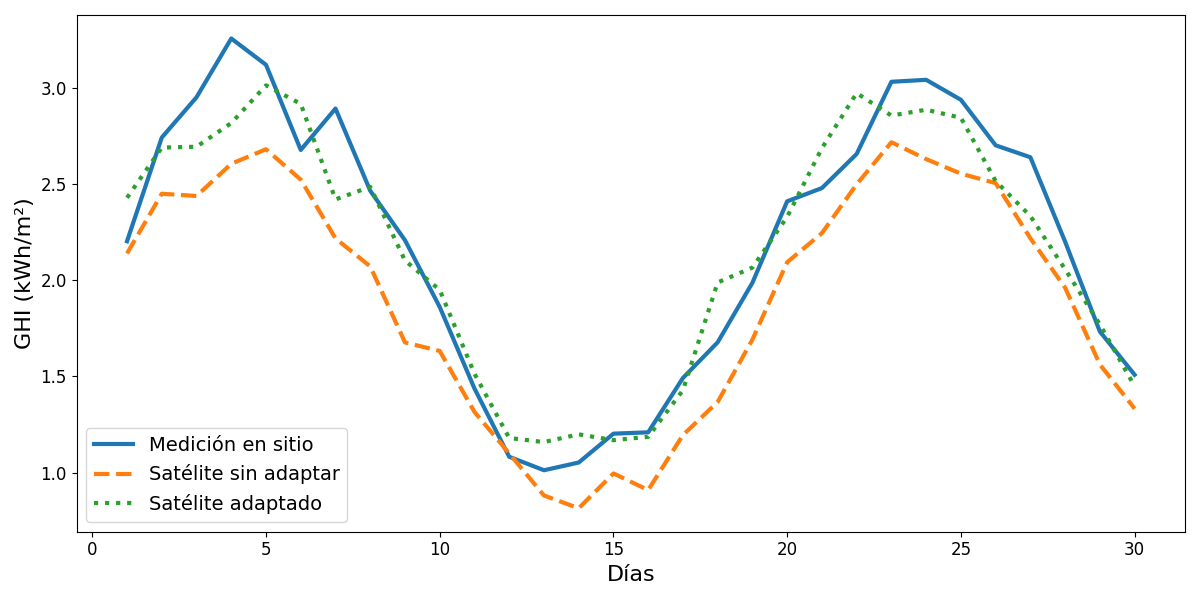
\includegraphics[width=0.97\linewidth]{figuras/SiteAdapation-Example.png}
    \caption{Comparación de irradiancia solar diaria entre datos de satélite sin adaptar, datos de satélite adaptados y mediciones locales en el sitio de referencia. Se observa cómo la adaptación al sitio corrige el sesgo sistemático y mejora la representatividad de los datos satelitales.}
    \label{fig:example}
\end{figure}


Dado que los datos modelados tienen errores, especialmente errores sistemáticos (sesgos) y errores aleatorios, esta técnica usa mediciones reales de radiación tomadas en el sitio (aunque sea durante un período corto) como referencia para calibrar los datos. El objetivo es reducir la incertidumbre y mejorar la precisión en las estimaciones de largo plazo.\\

La Figura \ref{fig:example}  ilustra una comparación entre tres conjuntos de datos de irradiancia solar a lo largo de un mes:

Medición en sitio (línea sólida): representa la referencia real tomada con instrumentos locales.

Satélite sin adaptar (línea discontinua): se observa un sesgo, ya que la serie está sistemáticamente desplazada respecto a la referencia. Además, los picos y valles no coinciden con exactitud, reflejando errores aleatorios.

Satélite adaptado (línea punteada): tras aplicar el procedimiento de adaptación al sitio, la serie corregida se ajusta mucho mejor a la referencia. El sesgo desaparece en gran medida y la forma de la curva sigue más de cerca la variabilidad de las mediciones locales.

Puede verse cómo la adaptación al sitio reduce tanto el error sistemático como la dispersión, logrando que los datos derivados de satélite sean más representativos de las condiciones reales de irradiancia en el lugar de interés.\\


\begin{figure}
    \centering
    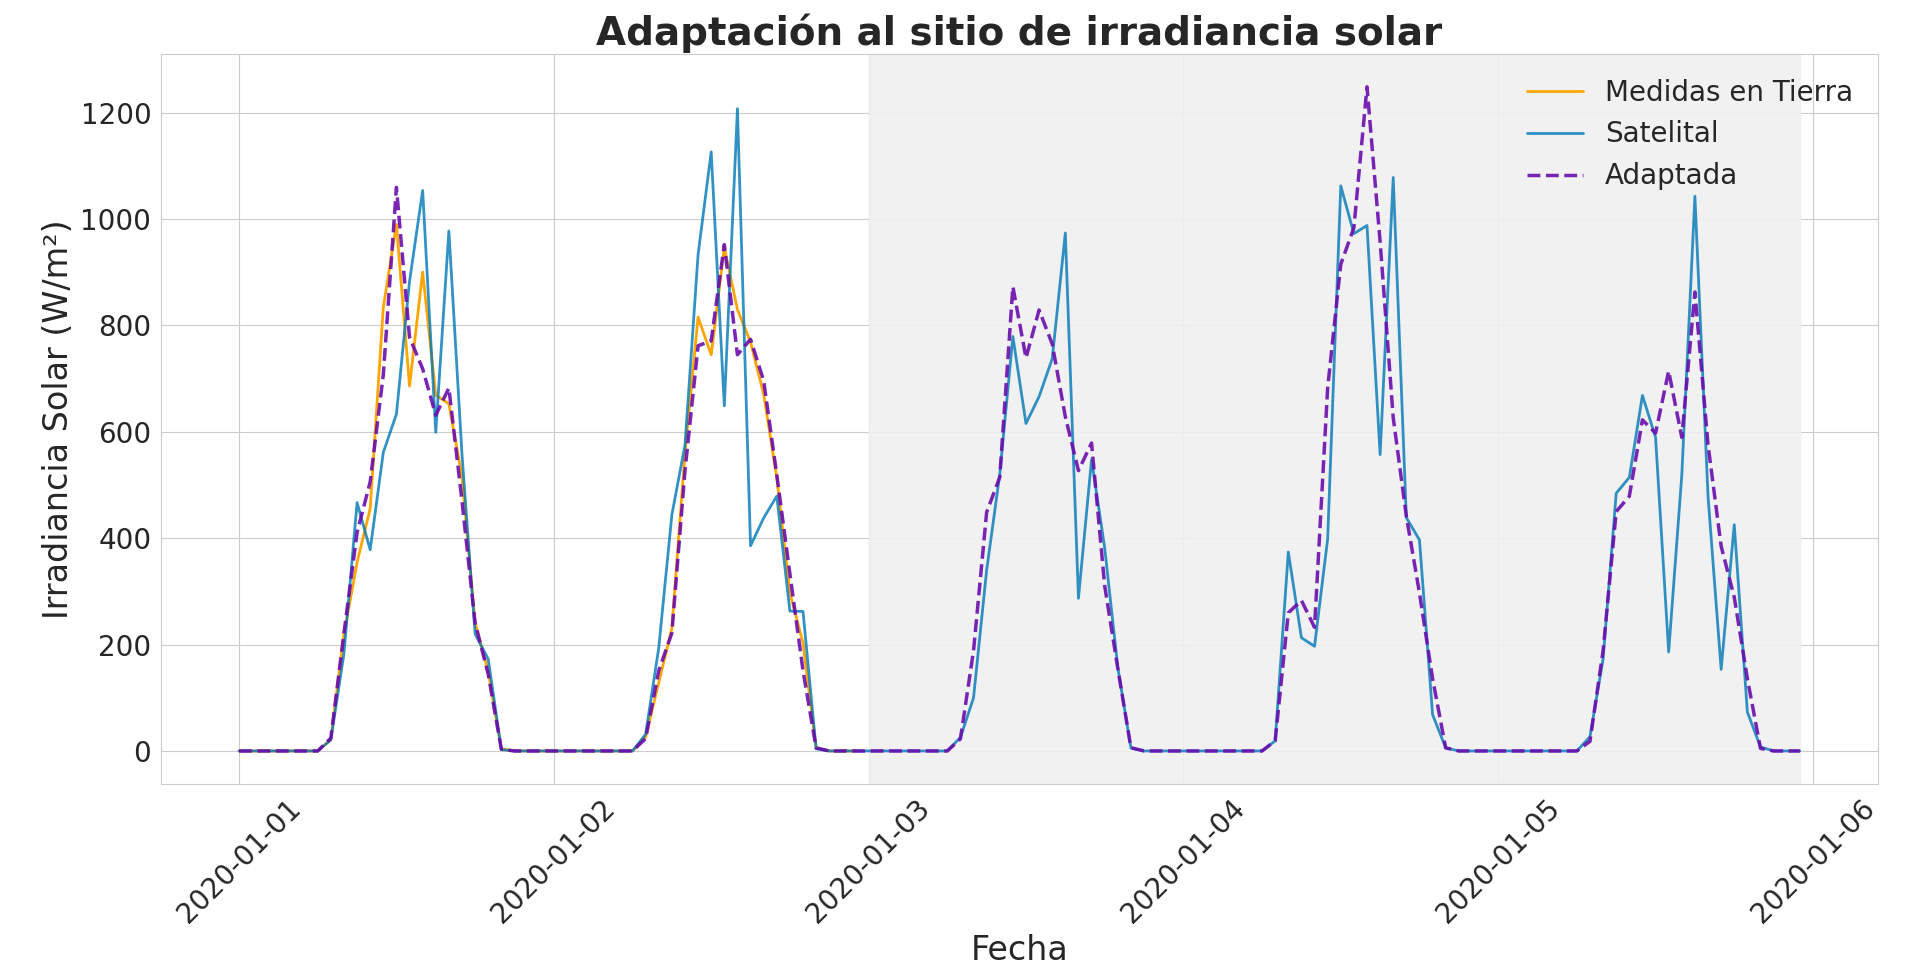
\includegraphics[width=0.97\linewidth]{figuras/siteAdaptation.png}
    \caption{Adaptación al Sitio sobre una serie genérica}
    \label{fig:site-adapation}
\end{figure}

En la Figura \ref{fig:site-adapation} puede verse el resultado que busca obtenerse al aplicar una adaptación al sitio. En color naranja se muestra la serie de medidas en tierra y en color azul la serie modelada, ambos casos con estilo de linea lleno. Debe tenerse en cuenta que el fondo cambiante de color (blanco y salmón) está realizado así a propósito.\\ 

Vamos a presentar una pequeña analogía que ayude a explicar de manera más cotidiana la idea general del preceso de SA.
\begin{quote}
Imagina que tienes un \textbf{termómetro económico} en tu casa (equivalente a los datos de un \textit{modelo}), 
pero al lado colocas uno profesional del hospital (equivalente a la \textit{medición en sitio}).  

Al comparar, notas que tu termómetro casero siempre marca \(-2\,^{\circ}\mathrm{C}\) respecto al valor real.  

Si corriges ese error sumando esos 2 grados, tu termómetro económico comienza a ser \textbf{útil y confiable} para el uso diario.  

\medskip
$\Rightarrow$ Eso es, en esencia, la \textbf{adaptación al sitio}: reducir el error de un modelo a partir de  una referencia local.
\end{quote}



\begin{figure}[H]
\centering
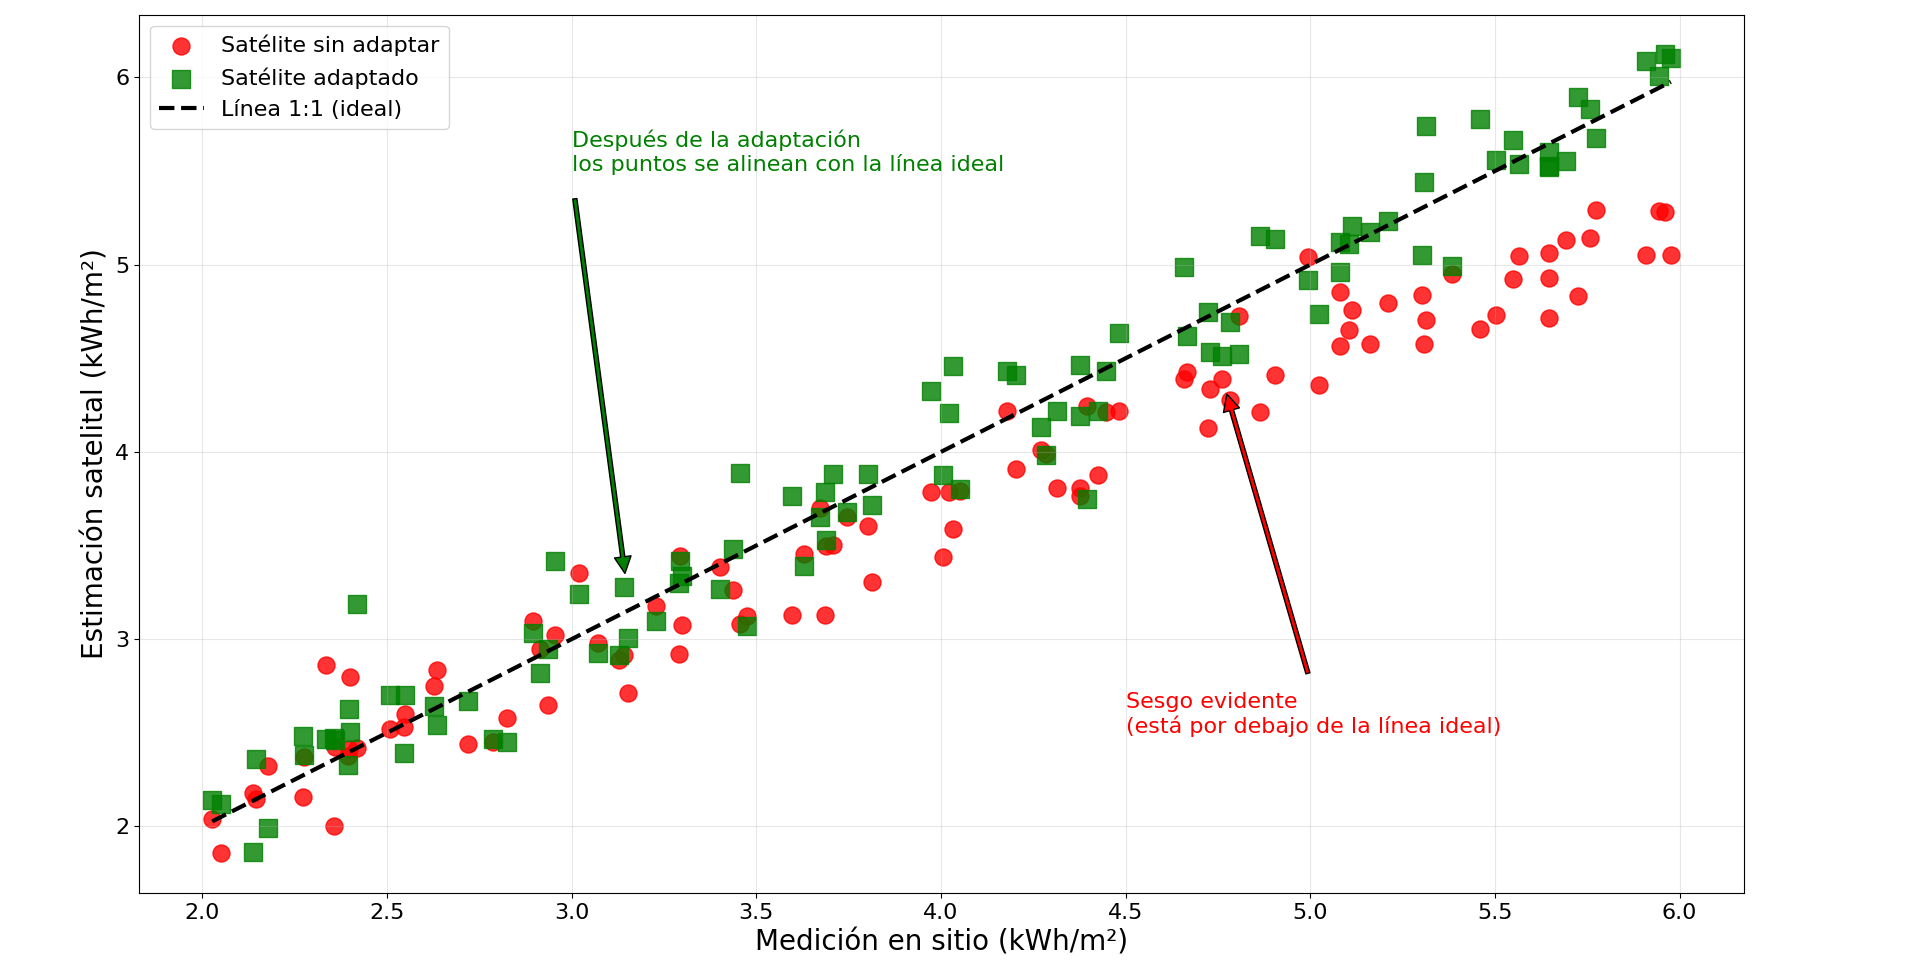
\includegraphics[width=\textwidth]{figuras/scatter-01.png}
\caption{Diagrama de dispersión entre mediciones en sitio y estimaciones satelitales.
Antes de la adaptación (puntos rojos), los datos muestran un sesgo claro al situarse por debajo de la línea 1:1. 
Después de la adaptación (puntos verdes), las estimaciones se alinean mucho mejor con la referencia, reduciendo el error sistemático.}
\label{fig:scatter01}
\end{figure}



La Figura \ref{fig:scatter01} muestra de manera evidente el efecto de la adaptación al sitio:

Antes de la corrección (rojo): los puntos están sistemáticamente alejados de la línea 1:1, lo que indica que el satélite subestima los valores reales de irradiancia. Existe un sesgo claro.

Después de la corrección (verde): los puntos se agrupan alrededor de la línea 1:1, lo que significa que las estimaciones satelitales ahora representan con mayor fidelidad las mediciones en sitio.




\section{Historia}
Uno de los principales aportes sobre el tema fue realizado en el trabajo de \cite{POLO2016} en el marco de la Tarea 46 del Programa de Calefacción y Refrigeración Solar de la Agencia Internacional de la Energía Evaluación y pronóstico de recursos solares. En este trabajo se indica que la idea general de este proceso de corrección o calibración de datos modelados es similar a lo que se ha desarrollado en  la industria eólica en el pasado \citep{Potter}.
 
Según Polo y sus colaboraores AS en un término actualmente utilizado en proyectos de energía solar para referirse a la mejora que puede lograrse en la irradiancia solar derivada de satélite y los datos del modelo cuando se utilizan mediciones terrestres locales a corto plazo para corregir errores sistemáticos y sesgos en el conjunto de datos original. A partir de esta idea general se han agrupado a los diversos métodos para SA en cinco categorías en las cuales se comprenden las principales estrategias para mejorar la precisión y reducir la incertidumbre en las estimaciones de radiación solar derivadas de satélites mediante el uso de mediciones locales de corta duración.

\begin{enumerate}
    \item Métodos basados en modelos físicos (Physically based methods)\\
        Ajustan los datos de entrada atmosféricos (como la turbidez por aerosoles o el vapor de agua) para que los resultados coincidan mejor con las observaciones en tierra. Ejemplos: uso del modelo REST2 y corrección del AOD (Aerosol Optical Depth)
    \item Métodos estadísticos (Statistical methods) \\
        Ajustan los datos del modelo para eliminar errores sistemáticos (sesgo) y mejorar la concordancia con datos medidos localmente.

        \begin{itemize}
            \item Eliminación de sesgo mediante adaptación lineal
            \item Métodos no lineales (transformación de características, polinomios, etc.)
            \item MOS (Model Output Statistics)
            \item MCP (Measure–Correlate–Predict)
            \item Adaptación regional (usando estaciones cercanas)
            \item Adaptación usando funciones de distribución acumulativa (CDF)
        \end{itemize}
        
    \item Adaptación de parámetros de entrada del modelo satelital \\
        Se modifican directamente los parámetros de entrada del modelo (como el índice de claridad o datos atmosféricos) en lugar de los resultados de irradiancia.
    \item Técnicas MCP aplicadas a datos satelitales y de reanálisis \\
        Uso de métodos de correlación-predicción (común en energía eólica) para extender los datos de corto plazo a largo plazo con apoyo en modelos de reanálisis.
        
    \item Combinación de datos satelitales con modelos meteorológicos numéricos (NWP)\\
        Mejora de la precisión mediante regresiones no paramétricas (como modelos aditivos generalizados - GAM) que combinan datos satelitales con modelos meteorológicos.
\end{enumerate}


Además de presentar la clasificación anterior, se han indicado algunas directrizces que deben ser tomadas en cuenta en un proceso de adaptación. \\



A partir del año 2020 se comenzaron a publicar diversos trabajos sobre Adaptación al Sitio (SA). En \citep{POLO2020} se presentan los resultados de adaptaciones realizadas en diez estaciones a escala horaria, considerando ocho modelos satelitales y dos de re-análisis. En \citep{Fernández2020} se evaluaron los resultados de la adaptación al sitio utilizando regresiones lineales múltiples (MLR) y se combinaron estos resultados con un ajuste mediante mapeo de cuantiles (QM). Este enfoque de ensamble de modelos mostró una reducción promedio del 1,7\% en el sesgo relativo y del 3,3\% en la desviación cuadrática media relativa a escala horaria. El estudio también sugiere que un año de datos es suficiente para entrenar los modelos de ajuste.

En el trabajo de \citep{BABAR2020} se evaluó el desempeño de la SA en los valores medios diarios del modelo satelital CLARA-A2 y del modelo de re-análisis ERA5. Para ello, se utilizó un modelo de Random Forest para la regresión, incorporando como predictores los valores de GHI modelados por CLARA-A2 y ERA5, sus respectivos índices de cielo despejado y el ángulo cenital solar medio. Los resultados demostraron una reducción de la desviación cuadrática media de 17,9 W/m² a 16,2 W/m² y una corrección completa del sesgo inicial de -1,5 W/m². La motivación para adoptar un modelo de regresión basado en aprendizaje automático surgió de la hipótesis de que este tipo de algoritmo podría aplicar funciones de regresión distintas a cada subconjunto del espacio de datos predictivos. Este trabajo es uno de los primeros en utilizar modelos de aprendizaje automático como Random Forest para determinar una función de ajuste que calibra las mediciones en tierra y puede aplicarse a series de largo plazo.

A partir del trabajo de Babar y colaboradores, se han publicado diversos estudios en los que se exploran modelos de aprendizaje automático como alternativa para determinar funciones de ajuste sobre series modeladas, ya sean satelitales o de re-análisis.

En \citep{NARVAEZ2021} se evaluó la adaptación al sitio en series horarias, explorando el uso de redes neuronales y los modelos Random Forest y AdaBoost. El rendimiento de estos modelos se evaluó en función de las métricas obtenidas en comparación con los ajustes realizados mediante QM y MLR, donde Random Forest logró una mejora aproximada del 38\% con respecto a QM y MLR.

En \citep{YANG2021} se presenta una alternativa denominada Adaptación al Sitio Probabilística, que aprovecha la disponibilidad de múltiples modelos de estimación simultáneamente. Este enfoque combina regresiones de cuantiles sobre múltiples modelos a la vez para mejorar la precisión de la adaptación al sitio.

En el trabajo de \citep{SALAMALIKIS2022}, se aplicó SA al modelo Heliosat-4 con una resolución horaria mediante el entrenamiento de diferentes modelos de regresión para condiciones de cielo despejado y nublado, considerando segmentos de datos basados en rangos de 15° del ángulo cenital solar. En este estudió se reportó  que el sesgo se redujo en un 50\% y la desviación cuadrática media disminuyó en un 3,8\% en comparación con las estimaciones sin SA. Los mejores resultados de este trabajo se obtuvieron utilizando modelos de regresión basados en árboles de decisión, en particular Random Forest. Además, una característica a destacar sobre este trabajo es que los autores han buscado eliminar la estacionalidad de la serie definiendo $\Delta_{GHI}$ como la diferencia entre la GHI medida y la GHI modelada. Esta variable se utiliza entonces como objetivo para los modelos de regresión, y la GHI adaptada se calcula como la suma del GHI modelada y $\Delta_{GHI}$. Puede considerarse que los autores en este trabajo han buscado quitar la \enquote{\textit{estacionalidad}} de la serie. Esta práctica es ampliamente conocida y estudiada en el área del análisis de series temporales, es recomendada y analizada en estudios como \citep{THORNTON2013, Claveria2015}.   


En \citep{ZAINALI2024} se evaluó un proceso de SA en tres sitios del norte de Europa utilizando diversos ajustes de mapeo de cuantiles y modelos de aprendizaje automático para ajustar los datos del modelo STRANG. Los hallazgos indican que los modelos de aprendizaje automático generalmente obtienen un rendimiento superior al de los métodos estadísticos, logrando una mejora de hasta el 9,2\% en la reducción del sesgo.




\section{Características}
\section{Ventajas y Desventajas}


\section{Modelos de Aprendizaje Automático} \label{MLM}
Aunque Arthur Samuel no fue el primero en publicar un artículo que empleara el término "aprendizaje automático", se le atribuye la creación y definición de este concepto como el campo especializado que conocemos hoy. En su trabajo `Algunos estudios sobre aprendizaje automático usando el juego de damas' \cite{samuel1959}, presentó el aprendizaje automático como una rama de la informática que permite a las computadoras mejorar su desempeño sin necesidad de ser programadas de forma explícita.

Si bien la definición original de Samuel no lo menciona directamente, un aspecto fundamental del aprendizaje automático es el autoaprendizaje. Este concepto implica el uso de modelos estadísticos para identificar patrones y optimizar el rendimiento con base en datos e información empírica, sin requerir instrucciones de programación explícitas \cite{Theobald2024}.

Samuel no infirió que las máquinas puedan tomar decisiones sin programación previa. Al contrario, el aprendizaje automático depende en gran medida de la entrada de código. En cambio, observó que las máquinas pueden realizar una tarea específica utilizando datos de entrada en lugar de depender de un comando de entrada directo.

\begin{figure}[H]
    \centering
    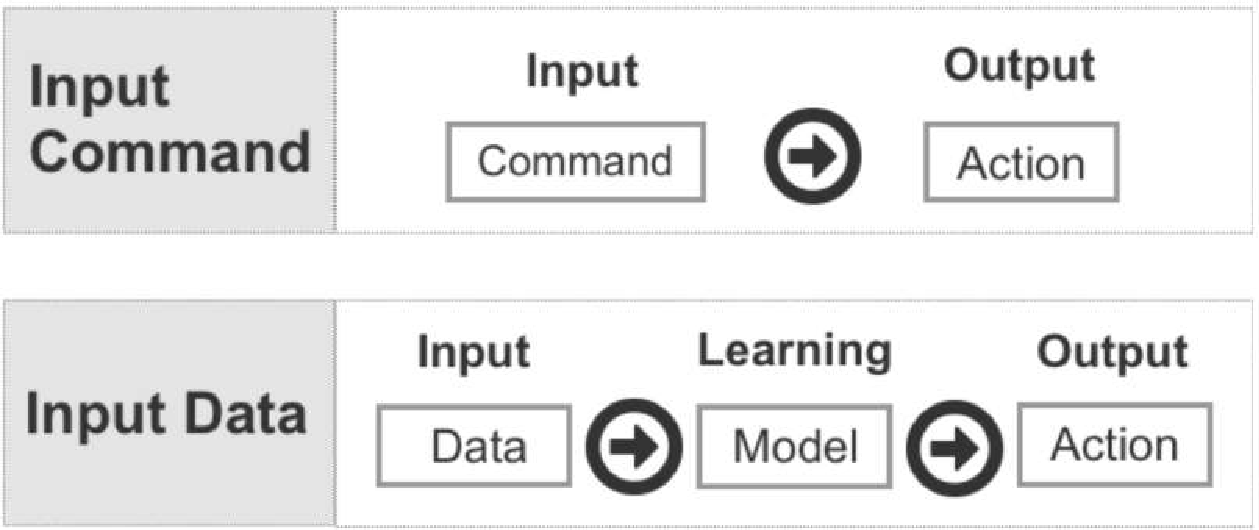
\includegraphics[scale=0.5]{figuras/ML.pdf}
    \caption{Comparación entre el comando de entrada y los datos de entrada}
    \label{fig:ML}
\end{figure}



\subsection{Modelo de red neuronal}

No existe una definición única de lo que es una red neuronal artificial, pero distintas fuentes proponen descripciones complementarias. Algunas de las más comunes son:

\begin{itemize}
    \item Un modelo computacional, paralelo, compuesto por unidades procesadoras adaptativas altamente interconectadas.
    \item Un sistema de procesamiento de la información que aplica principios inspirados en la organización del cerebro humano.
    \item Un modelo matemático diseñado para emular, de manera simplificada, el funcionamiento del cerebro.
    \item Un sistema de información con características de funcionamiento similares a las redes neuronales biológicas.
    \item Una red adaptativa que combina técnicas de procesamiento paralelo de la información.
    \item Una extensión de los métodos clásicos estadísticos, especialmente útil en el reconocimiento de patrones.
\end{itemize}

En todas estas definiciones se aprecia un componente de \textit{simulación biológica}. Las redes neuronales artificiales se inspiran en el cerebro humano en el sentido de que el procesamiento de la información se distribuye entre elementos básicos llamados \textit{neuronas}. Estas están interconectadas mediante \textit{pesos sinápticos}, que se ajustan a lo largo del tiempo durante un proceso denominado \textit{aprendizaje}. En términos simples, aprender consiste en modificar la intensidad de las conexiones entre neuronas para resolver una tarea determinada.

\subsubsection*{Neurona artificial}

Los componentes básicos de una neurona artificial son:

\begin{enumerate}
    \item Un conjunto de conexiones ponderadas (pesos sinápticos).
    \item Un sesgo, que actúa como umbral de activación.
    \item Un sumador, que agrega las entradas multiplicadas por sus pesos correspondientes.
    \item Una función de activación no lineal, que permite ampliar la capacidad de representación del modelo.
\end{enumerate}

\begin{figure}[H]
    \centering
    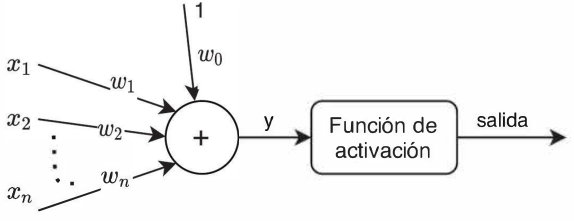
\includegraphics[scale=0.7]{figuras/neurona.png}
    \caption{Esquema de una neurona artificial}
    \label{fig:neurona}
\end{figure}

El funcionamiento matemático de una neurona artificial puede expresarse como:

\begin{equation}
    salida = f(y) = f\left( \sum_{k=0}^{n} w_{k}x_{k} \right)
    \label{eq:neurona}
\end{equation}

donde $x_i$ son las entradas, $w_i$ los pesos sinápticos y $x_0=1$ corresponde al sesgo con coeficiente $w_0$. La función $f$ representa la activación de la neurona.

\subsubsection*{Funciones de activación}

Las funciones de activación más comunes se resumen en la Tabla \ref{tab:activations}. Estas permiten introducir no linealidad en el modelo, lo cual es fundamental para que la red pueda aproximar funciones complejas.

\begin{table}[h]
    \centering
    \renewcommand{\arraystretch}{1.5}
    \begin{tabular}{|>{\centering\arraybackslash}p{2cm}|>{\centering\arraybackslash}p{5cm}|>{\centering\arraybackslash}p{8cm}|}
        \hline
        \textbf{Función} & \textbf{Expresión} & \textbf{Comentario} \\ 
        \hline
        Signo & 
        \( f(x) =
        \begin{cases} 
            1, & \text{si } x \geq 0 \\ 
            -1, & \text{si } x < 0 
        \end{cases} \)  
        & Usada en los primeros modelos de neuronas artificiales. \\ 
        \hline
        Sigmoide & 
        \( f(x) = \frac{1}{1 + e^{-x}} \)  
        & Transición suave entre 0 y 1, útil en clasificación binaria. \\ 
        \hline
        Tangente hiperbólica & 
        \( f(x) = \frac{e^x - e^{-x}}{e^x + e^{-x}} \)  
        & Similar a la sigmoide, pero con valores entre -1 y 1. \\ 
        \hline
        ReLU & 
        \( f(x) = \max(0, x) \)  
        & Una de las más usadas actualmente; evita problemas de gradiente. \\ 
        \hline
        Softmax & 
        \( f(x_i) = \frac{e^{x_i}}{ \sum_{k} e^{x_k} } \)  
        & Utilizada en la salida de modelos de clasificación multiclase. \\ 
        \hline
    \end{tabular}
    \caption{Funciones de activación más comunes en redes neuronales artificiales.}
    \label{tab:activations}
\end{table}

\subsubsection*{Perceptrón y sus limitaciones}

El perceptrón simple, basado en esta estructura, funciona como un clasificador binario que sólo puede resolver problemas linealmente separables. El procedimiento de aprendizaje consiste en:

\begin{enumerate}
    \item Inicializar aleatoriamente los pesos $w_{k}$.
    \item Establecer el parámetro de aprendizaje $\alpha$.
    \item Calcular la salida: $salida = signo(\sum_{k=0}^{n} w_{k} x_{k})$.
    \item Calcular el error: $error = salida_{deseada} - salida$.
    \item Actualizar los pesos: $w_{k} = w_{k} + \alpha \cdot error \cdot x_{k}$.
    \item Repetir el proceso.
\end{enumerate}

Aunque este modelo es simple y útil, su capacidad de representación es limitada. Para superar estas restricciones se introducen las redes \textbf{multicapa}.

\subsubsection*{Perceptrón Multicapa (MLP)}

El \textit{Perceptrón Multicapa} (MLP, por sus siglas en inglés) organiza neuronas en diferentes capas: una capa de entrada, una o varias capas ocultas y una capa de salida (Fig. \ref{fig:MLP}). Gracias a esta estructura, el MLP puede aproximar funciones no lineales y resolver problemas más complejos.

\begin{figure}[H]
    \centering
    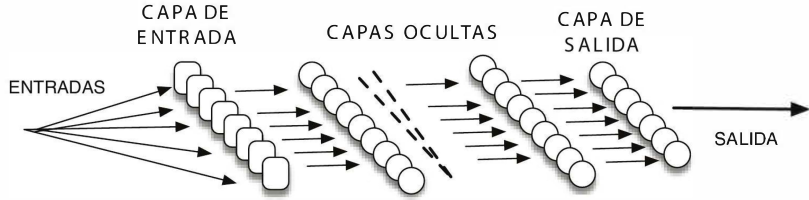
\includegraphics[scale=0.6]{figuras/MLP.png}
    \caption{Esquema de una red neuronal multicapa (MLP).}
    \label{fig:MLP}
\end{figure}

Un MLP con una capa oculta se puede definir como:

\begin{equation}
\hat{y} = f^{(2)}\Big( W^{(2)} \cdot f^{(1)}( W^{(1)} x + b^{(1)} ) + b^{(2)} \Big),
\end{equation}

donde $x$ es el vector de entrada, $W^{(1)}, W^{(2)}$ son matrices de pesos, $b^{(1)}, b^{(2)}$ los sesgos y $f^{(1)}, f^{(2)}$ las funciones de activación de cada capa \cite{ghanou2016mlp}.

\subsubsection*{MLP en la estimación de irradiancia solar}

En el contexto de la estimación de la irradiancia global horizontal (GHI), el MLP puede verse como un \textit{equipo de expertos neuronales}. Cada neurona aporta una “opinión parcial” a partir de las variables meteorológicas (nubosidad, humedad, ángulo solar, aerosoles), mientras que las capas ocultas integran estas opiniones para refinar la predicción de manera no lineal \cite{torobayona2012mlp}.  

\begin{figure}[H] 
\centering 
\begin{tikzpicture}[node distance=2.2cm]
\tikzstyle{neuron} = [circle, draw, minimum size=1cm, fill=blue!20, text centered]
\tikzstyle{output} = [rectangle, draw, thick, rounded corners, text centered, minimum height=1cm, minimum width=3cm, fill=green!20]

\node (input1) [neuron] {Nubosidad};
\node (input2) [neuron, below of=input1] {Humedad};
\node (input3) [neuron, below of=input2] {Ángulo solar};

\node (hidden1) [neuron, right of=input1, xshift=4cm] {Oculta 1};
\node (hidden2) [neuron, below of=hidden1] {Oculta 2};

\node (final) [output, right of=hidden1, xshift=4cm, yshift=-1cm] {Predicción de GHI};

\foreach \i in {input1,input2,input3}{
\foreach \j in {hidden1,hidden2}{
\draw[flecha] (\i.east) -- (\j.west);
}
}
\foreach \j in {hidden1,hidden2}{
\draw[flecha] (\j.east) -- (final.west);
}
\end{tikzpicture}
\caption{Analogía del MLP como un conjunto de expertos neuronales que refinan la predicción de la GHI.}
\label{fig:mlp_experts}
\end{figure}

El MLP ofrece una estructura potente y flexible capaz de modelar relaciones no lineales complejas, esto permite considerarlo como una herramienta adecuada para la estimación de irradiancia solar.

\subsubsection*{Ejemplo práctico de entrenamiento en un MLP}

Para ilustrar el funcionamiento del \textit{Perceptrón Multicapa} (MLP), consideremos un ejemplo sencillo con dos entradas, una capa oculta con dos neuronas y una salida (Figura \ref{fig:mlp_ejemplo}).  

\begin{figure}[H]
    \centering
    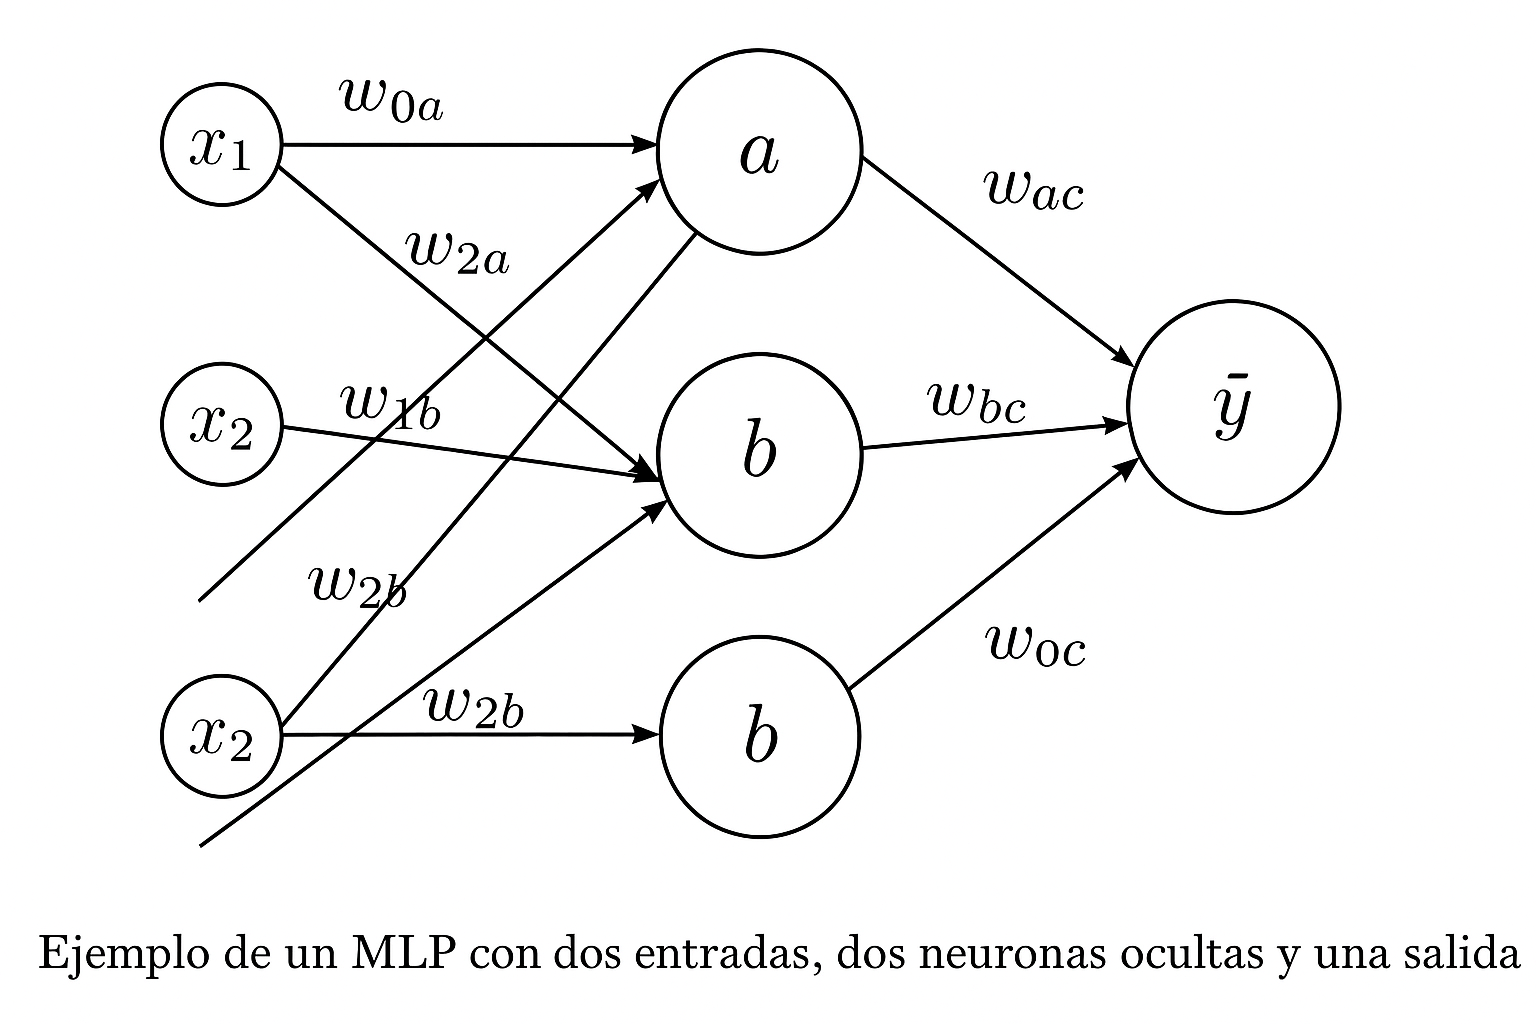
\includegraphics[scale=0.2]{figuras/mlp.png}
    \caption{Ejemplo de un MLP con dos entradas, dos neuronas ocultas y una salida.}
    \label{fig:mlp_ejemplo}
\end{figure}





El cálculo de las salidas se realiza en dos fases: propagación hacia adelante (\textit{forward pass}) y retropropagación del error (\textit{backpropagation}).

\paragraph{1. Propagación hacia adelante}
Las entradas $x_1$ y $x_2$ llegan a las dos neuronas ocultas $a$ y $b$:

\begin{equation}
    y_{a} = w_{0a} + w_{1a}x_{1} + w_{2a}x_{2}, \quad O_{a} = f(y_{a})
\end{equation}
\begin{equation}
    y_{b} = w_{0b} + w_{1b}x_{1} + w_{2b}x_{2}, \quad O_{b} = f(y_{b})
\end{equation}

Las salidas $O_{a}$ y $O_{b}$ alimentan a la neurona de salida $c$:

\begin{equation}
    y_{c} = w_{0c} + w_{ac}O_{a} + w_{bc}O_{b}, \quad \hat{y} = f(y_{c})
\end{equation}

donde $f(\cdot)$ es una función de activación diferenciable (sigmoide, tangente hiperbólica, ReLU, etc.).

\paragraph{2. Cálculo del error}
Dado un valor deseado $y$, el error cuadrático medio (ECM) para un ejemplo es:

\begin{equation}
    E = \frac{1}{2}(y - \hat{y})^2
\end{equation}

\paragraph{3. Retropropagación}
El objetivo es calcular cómo varía el error respecto a cada peso y ajustar estos valores en la dirección del gradiente descendente.

\begin{itemize}
    \item Para la salida $c$:
    \begin{equation}
        \delta_c = (y - \hat{y}) f'(y_{c})
    \end{equation}
    \item Para las neuronas ocultas $a$ y $b$:
    \begin{equation}
        \delta_a = f'(y_{a}) \cdot (w_{ac}\delta_c), \quad
        \delta_b = f'(y_{b}) \cdot (w_{bc}\delta_c)
    \end{equation}
\end{itemize}

\paragraph{4. Actualización de pesos}
Finalmente, los pesos se actualizan usando una tasa de aprendizaje $\eta$:

\begin{equation}
    w_{ij} \leftarrow w_{ij} + \eta \cdot \delta_j \cdot x_i
\end{equation}

donde $x_i$ es la entrada a la neurona $j$. Este procedimiento se repite para todos los ejemplos del conjunto de entrenamiento hasta que el error sea lo suficientemente pequeño.

\paragraph{5. Resumen del ciclo de aprendizaje}
\begin{enumerate}
    \item Inicializar pesos y sesgos aleatoriamente.
    \item Realizar la propagación hacia adelante para obtener la salida $\hat{y}$.
    \item Calcular el error $E$ comparando con el valor real $y$.
    \item Retropropagar el error para obtener los deltas $\delta$ de cada neurona.
    \item Actualizar los pesos usando la regla de gradiente descendente.
    \item Repetir el proceso hasta la convergencia.
\end{enumerate}

Este procedimiento es la base del entrenamiento de redes neuronales modernas. A pesar de su simplicidad, este esquema permite que los MLP aproximen relaciones altamente no lineales, siendo especialmente útiles para la estimación de la irradiancia solar, donde influyen múltiples variables meteorológicas de manera simultánea.













\subsection{Arboles de Decisión}
Los árboles de decisión son modelos no paramétricos (es decir que no se no toman suposiciones previas sobre la forma de distribución de los datos) que se utilizan principalmente para la resolución de problemas de clasificación o regresión. También son conocidos como árboles de clasificación y regresión (CART, classification and regression trees). Este tipo de modelo fue propuesto por Leo Breiman en el libro \cite{breiman1984}

Los árboles de decisión se basan en una serie de reglas de decisión para dividir el espacio de características predictoras en un número menor de regiones disjuntas en cada una de las cuales los valores de la variable respuesta son similares.

Un árbol de decisión parte del conjunto de datos de entrenamiento, correspondiente a un nodo raíz, y lo va dividiendo recursivamente en subconjuntos de datos homogéneos, dando lugar a nuevos nodos. La manera de formar los subgrupos es mediante la formulación de preguntas con respuesta binaria (si la variable respuesta es `jugar al tenis' se formula la pregunta ¿Sí o No juega al tenis?; si es `pesa más o menos de 75 kg.' la pregunta es ¿el peso es <=75 o >75?). \\

Los árboles de decisión se pueden clasificar en función del tipo de variable respuesta, si la variable de respuesta $y$ es cuantitativa el árbol es de regresión, si $y$ es cuantitativa el árbol es de clasificación.

\begin{figure}
    \centering
    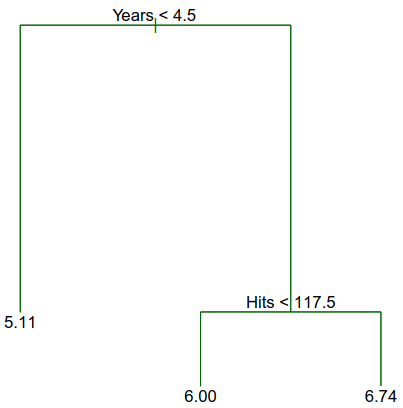
\includegraphics[width=0.25\linewidth]{figuras/tree_1.png}
    \caption{Ejemplo Árbol de Regresión. Para los datos de Hitters, se construye un árbol de regresión para predecir el logaritmo del salario de un jugador de béisbol, en función del número de años que ha jugado en las grandes ligas y el número de hits que realizó en el año anterior.}
    \label{fig:tree}
\end{figure}


El proceso general de construcción de un árbol de regresión puede describirse en dos pasos:
\begin{enumerate}
    \item  Dividir el espacio de predictores: es decir, el conjunto de valores posibles de $X_1, X_2, ..., X_p$ se divide en $J$ regiones distintas y no superpuestas, $R_1, R_2,..,R_J$.

    \item Hacer una predicción para cada región: para cada observación que cae en una región $R_j$, la predicción será simplemente la media de los valores de respuesta de las observaciones de entrenamiento dentro de $R_j$.
\end{enumerate}


\subsection{Random Forest}
\addcontentsline{toc}{subsection}{Random Forest: Un Enfoque de Aprendizaje Autom\'atico}

El algoritmo \textbf{Random Forest} (RF) es un modelo de aprendizaje supervisado de tipo \textit{ensemble} que se utiliza para resolver problemas de \textbf{clasificaci\'on} y \textbf{regresi\'on} \cite{louppe2015, salman2024}. Este m\'etodo, conceptualizado por Leo Breiman, es una extensi\'on del concepto de \textit{bagging} y se ha establecido como una t\'ecnica muy precisa y robusta en la miner\'ia de datos \cite{cutler2011}.


El fundamento de RF es la construcci\'on de un conjunto de m\'ultiples \'arboles de decisi\'on, donde cada \'arbol se entrena sobre un subconjunto de datos generado de forma aleatoria \cite{salman2024}. La aleatoriedad se introduce en dos niveles principales para garantizar que los \'arboles sean diversos y que el modelo no se sobreajuste:

\begin{enumerate}
    \item \textbf{Muestreo con reemplazo (Bootstrapping)}: Se generan m\'ultiples submuestras del conjunto de datos de entrenamiento original, con la posibilidad de que una misma observaci\'on aparezca varias veces en la misma submuestra. Cada submuestra se usa para entrenar un \'arbol de decisi\'on individual \cite{salman2024}.
    \item \textbf{Selecci\'on aleatoria de variables}: En cada nodo de un \'arbol, el algoritmo selecciona un subconjunto aleatorio de las variables predictoras disponibles. La mejor divisi\'on del nodo se determina a partir de este subconjunto reducido \cite{cutler2011, salman2024}. Esta t\'ecnica reduce la correlaci\'on entre los \'arboles y mejora la capacidad de generalizaci\'on del modelo \cite{cutler2011}.
\end{enumerate}


La divisi\'on \'optima en cada nodo del \'arbol se basa en la minimizaci\'on de una funci\'on de costo, que var\'ia seg\'un el tipo de problema.

Para problemas de \textbf{clasificaci\'on}, se utilizan medidas de impureza como el \textbf{\'indice Gini} o la \textbf{Entrop\'ia}. El \'Indice Gini mide la probabilidad de que una muestra elegida al azar de un nodo sea clasificada err\'oneamente, y se calcula de la siguiente manera:
$$
I_G(p) = 1 - \sum_{i=1}^{c} p_i^2
$$
donde $c$ es el n\'umero de clases y $p_i$ es la proporci\'on de muestras de la clase $i$ en el nodo.

Para problemas de \textbf{regresi\'on}, el criterio de divisi\'on se basa en la minimizaci\'on de la varianza o el \textbf{Error Cuadr\'atico Medio (MSE)} de las predicciones en los nodos hijos:
$$
MSE = \frac{1}{n} \sum_{i=1}^{n} (y_i - \hat{y}_i)^2
$$
donde $n$ es el n\'umero de muestras, $y_i$ es el valor real y $\hat{y}_i$ es el valor predicho.

Para realizar una predicci\'on final, el algoritmo agrega los resultados de todos los \'arboles del \textit{bosque} \cite{salman2024}. En problemas de \textbf{clasificaci\'on}, la predicci\'on se basa en el \textbf{voto mayoritario} de los \'arboles. Para problemas de \textbf{regresi\'on}, la predicci\'on final es el promedio de los resultados de cada \'arbol individual:
$$
\hat{y}_{RF}(\mathbf{x}) = \frac{1}{B} \sum_{b=1}^{B} h_b(\mathbf{x})
$$
donde $B$ es el n\'umero total de \'arboles en el bosque y $h_b(\mathbf{x})$ es la predicci\'on del $b$-\'esimo \'arbol.


Random Forest ofrece varias ventajas significativas para el an\'alisis de datos \cite{cutler2011}:

\begin{itemize}
    \item \textbf{Resistencia al sobreajuste (\textit{overfitting})}: El algoritmo es intr\'insecamente resistente al sobreajuste, ya que el conjunto de \'arboles se entrena en subconjuntos aleatorios de datos \cite{salman2024}.
    \item \textbf{Manejo de variables}: Es capaz de manejar eficientemente un gran n\'umero de variables, incluso cuando hay valores perdidos, sin necesidad de imputaci\'on previa \cite{cutler2011}.
    \item \textbf{Estimaci\'on de la importancia de las variables}: El algoritmo proporciona una medida integrada que indica la contribuci\'on relativa de cada variable al modelo, lo que facilita la interpretaci\'on de los resultados \cite{cutler2011}.
\end{itemize}



\subsection{XGBoost}

El algoritmo \textit{Extreme Gradient Boosting} (XGBoost) es una implementación optimizada del método de \textit{Gradient Boosted Decision Trees} (GBDT) \cite{chen2016xgboost}.
Su funcionamiento consiste en combinar múltiples árboles de decisión simples para construir un modelo robusto, de manera semejante a cómo un equipo de especialistas aporta su conocimiento colectivo para tomar mejores decisiones.
XGBoost se ha consolidado como estado del arte en aprendizaje automático debido a su alto desempeño en tareas de clasificación y regresión en diversos dominios \cite{espinoza2020aplicacion}.\\


Para entender el algoritmo y su aplicación en la estimación de la GHI, podemos usar una analogía. Supongamos que deseamos predecir la GHI en un lugar específico.

Un único árbol de decisión actúa como un \textit{experto solitario}, que utiliza reglas simples para emitir un juicio, por ejemplo: \`si la nubosidad es alta, entonces la irradiancia será baja''. Aunque este razonamiento es útil, tiene limitaciones: la irradiancia también depende de la altura solar, aerosoles, humedad relativa o estacionalidad. Por ello, un solo árbol puede fallar al no capturar la complejidad completa del fenómeno.

XGBoost supera esta limitación mediante un \textit{comité de expertos}, es decir, un conjunto de árboles que se construyen secuencialmente para aprender de los errores de sus predecesores. Cada árbol nuevo se centra en corregir las predicciones incorrectas de los anteriores, especializándose en las regiones donde estos fallaron. Así, el modelo colectivo refina sus predicciones de manera progresiva. Esta dinámica se ilustra en la Figura \ref{fig:xgb_experts}.

Podemos compararlo con un proceso de deliberación científica: el primer investigador propone un modelo básico; otro detecta que no captura los días parcialmente nublados y lo corrige; un tercero ajusta los errores en días despejados con baja humedad. Con el tiempo, el grupo obtiene un modelo más completo que cualquiera de los expertos individuales.\\

Esta idea refleja la esencia del \textit{gradient boosting}: aprendizaje aditivo y secuencial, donde cada árbol se incorpora para reducir la pérdida residual del conjunto previo \cite{chen2016xgboost}. La fuerza del modelo final no está en la exactitud de cada árbol individual (clasificador débil), sino en la sinergia de todos ellos, formando un predictor colectivo altamente robusto.
En el caso de la estimación de GHI, el ensamble de árboles de XGBoost permite capturar relaciones complejas entre variables meteorológicas y solares, mientras controla el sobreajuste mediante regularización y técnicas adicionales como \textit{shrinkage} y submuestreo \cite{xgboostdoc}.

En resumen, si un árbol es un experto solitario con visión parcial, XGBoost funciona como un \textit{panel de expertos} que deliberan y corrigen mutuamente sus errores para alcanzar predicciones más precisas.

\begin{figure} \centering \begin{tikzpicture}[node distance=2.2cm] % Estilos de nodos
\tikzstyle{expert} = [rectangle, draw, rounded corners, text centered, text width=3.5cm, minimum height=1cm, fill=blue!15] \tikzstyle{consensus} = [rectangle, draw, thick, rounded corners, text centered, text width=4.5cm, minimum height=1.2cm, fill=green!20] % Nodos de expertos 
\node (exp1) [expert] {Árbol 1:\\ Si nubosidad alta $\Rightarrow$ baja irradiancia''}; \node (exp2) [expert, below of=exp1] {Árbol 2:\\ Corrige error en días despejados}; \node (exp3) [expert, below of=exp2] {Árbol 3:\\ Ajusta casos con alta humedad}; \node (exp4) [expert, below of=exp3] {Árbol 4:\\ Mejora predicción en invierno}; % Nodo de consenso 
\node (final) [consensus, right of=exp2, xshift=8cm, yshift=-1cm] {Consenso del Comité (XGBoost):\\ Predicción refinada de GHI}; % Flechas de cada experto al consenso 
% Definir un estilo para las flechas \usetikzlibrary{decorations.markings} 
% cargar librería 
\tikzset{ flecha/.style={ thick, postaction={decorate, decoration={ markings, mark=at position 1 with {\arrow{>}} }} } } 
% Dibujar las flechas para los nodos exp1, exp2, exp3, exp4 hacia final
\foreach \i in {1,2,3,4}{ \draw[flecha] (exp\i.east) -- +(2,0) |- (final.west); } \end{tikzpicture} \caption{Analogía del comité de expertos en XGBoost: cada árbol corrige los errores de sus predecesores y contribuye a una predicción final más precisa de la GHI.} \label{fig:xgb_experts} \end{figure}

Formalmente, el modelo se define como:

\begin{equation}
\hat{y}_i = \sum_{k=1}^{K} f_k(x_i), \quad f_k \in \mathcal{F}, 
\end{equation}

donde cada $f_k$ es un árbol de regresión (\textit{CART}) y $\mathcal{F}$ es el espacio de todos los árboles posibles. La función objetivo combina el error de predicción y la complejidad del modelo:

\begin{equation}
\mathcal{L} = \sum_{i=1}^{n} l(y_i, \hat{y}_i) + \sum_{k=1}^{K} \Omega(f_k), 
\end{equation}

con regularización definida como:

\begin{equation} 
\Omega(f) = \gamma T + \frac{1}{2}\lambda \|w\|^2, 
\end{equation}

donde $T$ es el número de hojas, $w$ los pesos de cada hoja, $\gamma$ penaliza la complejidad del árbol y $\lambda$ regula la magnitud de los pesos \cite{chen2016xgboost}.


% Nuevo TikZ para árbol simple 
\begin{figure}[H] 
\centering 
\begin{tikzpicture}[sibling distance=12em, every node/.style = {shape=rectangle, rounded corners, draw, align=center, top color=white, bottom color=blue!20}] 
\node {Nubosidad $<$ 50\%?} child { node {Sí \\ $\Rightarrow$ Alta irradiancia} } child { node {No \\ $\Rightarrow$ Baja irradiancia}};
\end{tikzpicture} 
\caption{Ejemplo de un árbol de decisión simple. XGBoost combina cientos de estos árboles débiles para construir un modelo poderoso.} 
\label{fig:treeexample} 
\end{figure}

XGBoost entrena los árboles de manera \textit{aditiva}, es decir, cada iteración añade un árbol que corrige los errores acumulados. Para ello utiliza una expansión de segundo orden de la función objetivo:

\begin{equation} 
\mathcal{L}^{(t)} \approx \sum_{i=1}^n \left[ g_i f_t(x_i) + \frac{1}{2} h_i f_t^2(x_i) \right] + \Omega(f_t), 
\end{equation}

donde $g_i$ y $h_i$ son el gradiente y la segunda derivada de la función de pérdida en la predicción previa. Esta formulación otorga estabilidad y precisión al proceso de entrenamiento \cite{chen2016xgboost}.


El proceso iterativo se representa en la Figura \ref{fig:boosting}.

% TikZ proceso iterativo 
\begin{figure}[H] 
\centering 
\begin{tikzpicture}[node distance=2cm] % Nodos de iteración 
\node[rectangle, draw, fill=blue!20, rounded corners, minimum width=3cm, minimum height=1cm] (tree1) {Árbol 1: predicción inicial}; \node[rectangle, draw, fill=blue!20, rounded corners, minimum width=3cm, minimum height=1cm, below of=tree1] (tree2) {Árbol 2: corrige errores del árbol 1}; \node[rectangle, draw, fill=blue!20, rounded corners, minimum width=3cm, minimum height=1cm, below of=tree2] (tree3) {Árbol 3: corrige errores acumulados}; % Nodo de modelo final 
\node[rectangle, draw, fill=green!20, rounded corners, minimum width=4cm, minimum height=1cm, right of=tree2, xshift=6cm] (finalmodel) {Modelo XGBoost final}; 
% Flechas 
\foreach \i/\j in {tree1/finalmodel, tree2/finalmodel, tree3/finalmodel}{ \draw[flecha] (\i.east) -- (\j.west); } 
\end{tikzpicture} 
\caption{Proceso iterativo: cada nuevo árbol corrige los errores del modelo acumulado.} 
\label{fig:boosting} 
\end{figure}


XGBoost también incluye estrategias adicionales para mejorar la generalización \cite{xgboostdoc}:

\begin{itemize} 
\item \textbf{Shrinkage ($\eta$):} funciona como una `moderación'' en las decisiones del comité, reduciendo el impacto de cada nuevo árbol. 
\item \textbf{Submuestreo:} cada árbol se entrena con una muestra parcial de datos y características, como consultar a un subgrupo de expertos para ganar diversidad en las opiniones. 
\item \textbf{Regularización adicional:} actúa como una \textit{disciplina} que limita la complejidad de cada experto, evitando que se vuelva demasiado específico. 
\end{itemize}

En este estudio se utilizó la librería \texttt{xgboost} \cite{xgboostdoc}, con soporte para paralelización y GPU, lo que permitió un entrenamiento eficiente incluso con grandes volúmenes de datos. Los principales hiperparámetros (\texttt{max\_depth}, \texttt{eta}, \texttt{n\_rounds}, $\lambda$, $\gamma$) se ajustaron mediante \textit{grid search}.

De acuerdo a las especificaciones teóricas presentadas, consideramos que el uso de XGBoost es especialmente adecuado para el análisis de irradiancia solar porque:

\begin{enumerate}
\item Captura relaciones no lineales entre variables atmosféricas y solares.
\item Reduce el sobreajuste mediante mecanismos internos de regularización.
\item Permite escalabilidad y eficiencia en grandes bases de datos.
\item Suele superar a otros ensambles como Random Forest \cite{espinoza2020aplicacion}.
\end{enumerate}

% TikZ esquema conceptual 
\begin{figure}[H] 
\centering 
\begin{tikzpicture}[node distance=1.5cm] \node[rectangle, draw, fill=blue!20, rounded corners, minimum width=3cm, minimum height=0.8cm] (t1) {Árbol 1}; \node[rectangle, draw, fill=blue!20, rounded corners, minimum width=3cm, minimum height=0.8cm, below of=t1] (t2) {Árbol 2}; \node[rectangle, draw, fill=blue!20, rounded corners, minimum width=3cm, minimum height=0.8cm, below of=t2] (t3) {Árbol 3}; \node[rectangle, draw, fill=green!20, rounded corners, minimum width=4cm, minimum height=1cm, right of=t2, xshift=6cm] (final) {Predicción colectiva XGBoost}; \foreach \i in {t1,t2,t3}{ \draw[flecha] (\i.east) -- +(2,0) |- (final.west); } \end{tikzpicture} \caption{Esquema conceptual: múltiples árboles (\textit{expertos}) corrigen iterativamente sus errores para formar un modelo robusto.} \label{fig:esquemaxgb} \end{figure}


La Figura \ref{fig:esquemaxgb} resumen la idea para una predicción generica utilizando XGBoost como modelo regresor.


En resumen, mientras que un árbol de decisión actúa como un experto solitario y XGBoost combina múltiples árboles secuencialmente, un MLP funciona como un sistema de neuronas interconectadas que colectivamente aprenden patrones complejos en los datos, logrando predicciones precisas de irradiancia solar.



 %Obligatorio
\lhead{Capítulo \ref{ch_3}}
%\rhead{\newtitle}
\rhead{}
\cfoot{\thepage}
\renewcommand{\headrulewidth}{1pt}
\renewcommand{\footrulewidth}{1pt}
\chapter{Adaptación al Sitio en NOA}\label{ch_3}


En este capítulo se presentan los resultados obtenidos a partir de las distintas evaluaciones realizadas a la AS. 

\section{Medidas en tierra}


Los sitios analizados en esta tesis se resumen en la Tabla \ref{tab:sites}, donde se incluyen sus códigos de identificación, coordenadas geográficas, altitud sobre el nivel del mar, periodos de medición, clasificación climática según Köppen–Geiger \cite{peel2007} y el tipo de piranómetro utilizado. Estas estaciones  están ubicadas en el noroeste de Argentina como puede verse en la Figura \ref{fig:sites} y abarcan diversas condiciones climáticas y geográficas, que van desde tierras bajas subtropicales hasta altiplanos andinos de gran altitud.

\begin{figure}
   \centering
   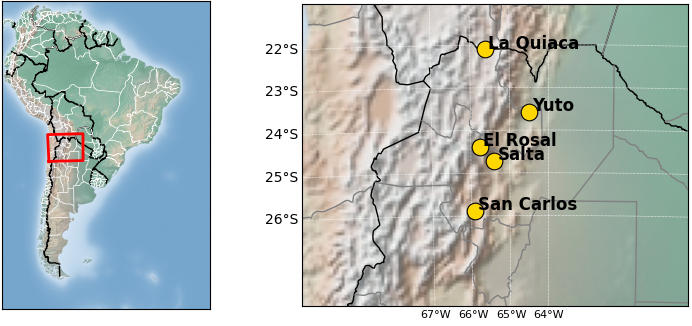
\includegraphics[width=1\linewidth]{figuras/sites.png}
    \caption{Ubicación de la estaciones de medida}
    \label{fig:sites}
\end{figure}


La estación Sa se encuentra en el campus experimental del INENCO, en la Universidad Nacional de Salta. Está situada en un entorno urbano preandino dentro del Valle de Lerma, una zona donde es común la formación de nubes debido a la cercanía de la cordillera. Su clima es subtropical de montaña, con inviernos secos y veranos frescos (Cwb). Las mediciones se realizaron entre 2009 y 2020 utilizando un piranómetro Eppley PSP.\\

La estación Lq, localizada en La Quiaca, presenta un clima estepario frío semiárido (BSk) típico de regiones andinas, y destaca por registrar uno de los mayores niveles de horas de sol anuales en Argentina. Contó con un piranómetro Kipp \& Zonen CMP11 y recopiló datos entre 2018 y 2023.

La estación Yu, ubicada en una zona de clima subtropical húmedo (Cwa), registró datos entre 2017 y 2018 con un sensor CMP11. La estación Sca, también con clima Cwb, operó entre 2012 y 2013 con un piranómetro CMP3. Finalmente, la estación Ero, situada en una región de gran altitud con clima BSk, recopiló datos entre 2016 y 2018, igualmente con un CMP3.

Todas las estaciones utilizan piranómetros que cumplen con los estándares de la norma ISO 9060:2018 Clase A o B para la medición de la irradiancia global horizontal (GHI). Los datos se registraron a intervalos de un minuto, y cada valor corresponde al promedio de seis muestras tomadas cada 10 segundos.




\begin{table}
    \centering
    \renewcommand{\arraystretch}{1.5} % Espaciado vertical en la tabla
    \begin{tabular}{|>{\centering\arraybackslash}p{2cm}|>{\centering\arraybackslash}p{2cm}|>{\centering\arraybackslash}p{2cm}|>{\centering\arraybackslash}p{2cm}|>{\centering\arraybackslash}p{2cm}|>{\centering\arraybackslash}p{2cm}|>{\centering\arraybackslash}p{2cm}|}
        \hline
        \textbf{ID} & \textbf{Provincia} & \textbf{Localidad} & \textbf{Latitud} & \textbf{Longitud}& \textbf{Altitud (m.s.n.m}) & \textbf{Clima}\\ 
        \hline

        \textbf{Yu} & Jujuy & Yuto & -23.58 & -64.5 & 401 & \textbf{Cwa}\\ 
        \textbf{Sa} & Salta & Salta & -24.72 & -65.4 & 1233 & \textbf{Cwb}\\ 
        \textbf{Sca} & Salta & San Carlos & -25.8951 & -65.925 & 1624 & \textbf{Cwb}\\
        \textbf{Er} & Salta & El Rosal & -24.39278 & -65.76806 & 3355& \textbf{Bsk}\\
        \textbf{Lq} & Jujuy & La Quiaca & -24.39278 & -65.76806 & 3355& \textbf{Bsk}\\
        \hline
        
        
    \end{tabular}
    \caption{Estaciones de medidas utilizadas en este trabajo}
    \label{tab:sites}
\end{table}




\subsection{Control de Calidad en las Medidas}

Las medidas fueron sometidas a un control de calidad (QC) siguiendo un procedimiento simplificado basado en \cite{Nollas2023}, con una etapa preliminar de filtrado por inspección visual según las recomendaciones de \cite{abal2020}. Dado que este estudio se basa únicamente en mediciones de irradiancia global horizontal (GHI) y no incluye componentes difusas, se aplicó una versión reducida del procedimiento original. 

La Tabla \ref{tab:qc} resume los filtros utilizados, donde $E$ es la constante solar, $S$ el factor de corrección de la distancia Tierra–Sol, $\theta_z$ el ángulo cenital solar y $kt$ el índice de claridad, definido como la razón entre la GHI y la irradiancia teórica en el tope de la atmósfera sobre un plano horizontal.\\

\begin{table}[h!]
\caption{Filtros de control de calidad aplicados a las mediciones.}
\label{tab:qc}
\centering
\resizebox{\linewidth}{!} {
\def\arraystretch{1.5}
\begin{tabular}{cc}
\hline
\textbf{Filtro} & \textbf{Descripción}\\ 
\hline
F1 & $GHI < 1.5~E~S~(\cos(\theta_z))^{1.2} + 100 \, \text{W/m}^2$  \\
F2 & $GHI > (6.5331 - 0.065502~\theta_z + 1.8312\text{E-4}~\theta_z^2)/(1 + 0.01113~\theta_z)$ \\
F3 & $kt < 1.4$ \& $ (90-\theta_z) < 10^\circ$  \\
\hline
\end{tabular}}
\end{table}

Los filtros aplicados pueden describirse de la siguiente manera:

\begin{itemize}
    \item \textbf{F1}: Rechaza valores que superan un límite físicamente razonable en función de la posición solar.
    \item \textbf{F2}: Descarta mediciones utilizando un umbral empírico dependiente del ángulo cenital.
    \item \textbf{F3}: Elimina valores del índice de claridad superiores a 1.4 cuando el Sol se encuentra a menos de $10^\circ$ sobre el horizonte.
\end{itemize}

El porcentaje de datos diurnos retenidos varió entre estaciones. En particular, el 73\% de los registros de Yu cumplieron los criterios establecidos, frente al 82\% en Sa, 72\% en Sca, aproximadamente 84\% en Ero y 69\% en Lq.





\subsection{Métricas de desempeño}

Los indicadores de desempeño más comunes en el campo de la evaluación del recurso solar han sido abordados por ~\cite{ZHANG}; estos incluyen el Error Medio de Sesgo (MBE), el Error Medio Absoluto (MAE) y el Error Cuadrático Medio (RMSE). Las tres métricas se definen de la siguiente manera:

\begin{equation}
\text{MBE} = \frac{\sum_{i=1}^{n} ( {y_i} - {x_i} ) }{n},
\end{equation}

\begin{equation}
\text{MAE} = \frac{\sum_{i=1}^{n} |{y_i} - {x_i} | }{n},
\end{equation}

\begin{equation}
\text{RMSE} = \sqrt{\frac{1}{n} \sum_{i=1}^{n} \Big({y_i - x_i}\Big)^2},
\label{ec:rrmsd}
\end{equation}

\noindent
donde $x$ y $y$ son los valores medidos y estimados, respectivamente, y $n$ es el tamaño de la muestra. El MBE mide el sesgo sistemático que un modelo puede introducir en una evaluación a largo plazo, mientras que el MAE y el RMSE miden la dispersión del error utilizando normas absolutas y cuadráticas, respectivamente. Debido a su mayor sensibilidad a los valores atípicos, el RMSE se utiliza frecuentemente en esta área. Ambas métricas de dispersión se reportan aquí por completitud. Los tres indicadores se presentan en términos relativos como un porcentaje del promedio de los valores medidos, denominados aquí como MBE (\%), MAE (\%) y RMSE (\%).




\section{Desempeño de los modelos de GHI en el NOA}
Previo a la presentación del desempeño de los distintos procesos de adaptación al sitio se evaluaron los modelos de estimación de GHI disponibles en la región. Siendo este uno de los aportes que se pretende en este trabajo. A continuación se muestran las métricas de desempeño de los modelos calculadas sobre el conjunto de datos de de cada sitio.



% Antes de la tabla, si quieres aumentar la altura de filas
\renewcommand{\arraystretch}{1.5}



\begin{table*}%[]
  \centering
  \caption{Métricas de desempeño (MBE, MAE, RMSE) para cada modelo y conjunto de datos satelitales en los cinco sitios. 
           Los valores están normalizados y expresados como porcentajes relativos al promedio de GHI en cada sitio: 
           396.8~W/m$^{2}$ (Yu), 397~W/m$^{2}$ (Sa), 557.1~W/m$^{2}$ (Sca), 690.6~W/m$^{2}$ (Ero) y 673.7~W/m$^{2}$ (Lq).}
  \resizebox{\linewidth}{!}{%
    \begin{tabular}{|l|ccc|ccc|ccc|ccc|ccc|}
      \hline
      & \multicolumn{3}{c|}{YU} & \multicolumn{3}{c|}{SA} & \multicolumn{3}{c|}{SCA} & \multicolumn{3}{c|}{ERO} & \multicolumn{3}{c|}{LQ} \\
      \cline{2-16}
      Modelo  & MBE & MAE & RMSE & MBE & MAE & RMSE & MBE & MAE & RMSE & MBE & MAE & RMSE & MBE & MAE & RMSE \\
      \hline
      \multicolumn{16}{|c|}{\textit{Resolución Temporal: 15 minutos}} \\
      \hline
      CAMS    & 0.5  & 18.4 & 28.4 & 3.5  & 23.9 & 33.2 & 2.7  & 23   & 30.4 & -23.7& 27.8 & 41.2 &-7.3 & 16.2 & 25.3 \\
      LSA-SAF & 10.7 & 19   & 28.8 & 17.3 & 26.9 & 38.8 & 11.5 & 22.2 & 30.6 & -8.1 & 16.5 & 26.8 & 3.7 & 12.3 & 22.3\\
      \hline
      \multicolumn{16}{|c|}{\textit{Resolución Temporal: horaria}} \\
      \hline
      CAMS    &  0.5 & 16   & 24.1 & 3.6  & 20.5 & 28.8 & 2.9  & 21   & 27.3 & -23.7& 26.8 & 39.5 & -6.1& 14.6 & 22\\
      LSA-SAF & 10.7 & 16.9 & 24.9 & 17.3 & 24.8 & 35   & 11.6 & 20.5 & 27.1 & -8.1 & 15   & 24.3 & 4.6 & 10.9 & 18.7\\
      ERA-5   & -4.2 & 45.4 & 61.9 & 8.5  & 26.8 & 37.5 & 7.4  & 21.2 & 28.9 & -13.7& 19.1 & 25.3 & -1.7& 12   & 19.3\\
      MERRA-2 & 26.9 & 35   & 51.9 & 42.1 & 47   & 63.6 & 12.7 & 21.9 & 29.3 & -3.1 & 13.1 & 20.5 & 1.0 & 13.4 & 21.1\\
      \hline
    \end{tabular}%
  }
\end{table*}
    


\subsection{Análisis de las estimaciones 15-minutales}

La Figura \ref{fig:general-15} muestra la evaluación comparativa de los modelos CAMS y LSA-SAF en los sitios de estudio. En el caso del MBE, se observa que LSA-SAF presenta sesgos positivos en la mayoría de los sitios, indicando una tendencia a la sobreestimación sistemática de las variables simuladas, mientras que CAMS exhibe valores más cercanos a cero o incluso negativos, lo que refleja un comportamiento más balanceado, aunque con subestimaciones marcadas en sitios como Er y Lq.


\begin{figure}
    \centering
    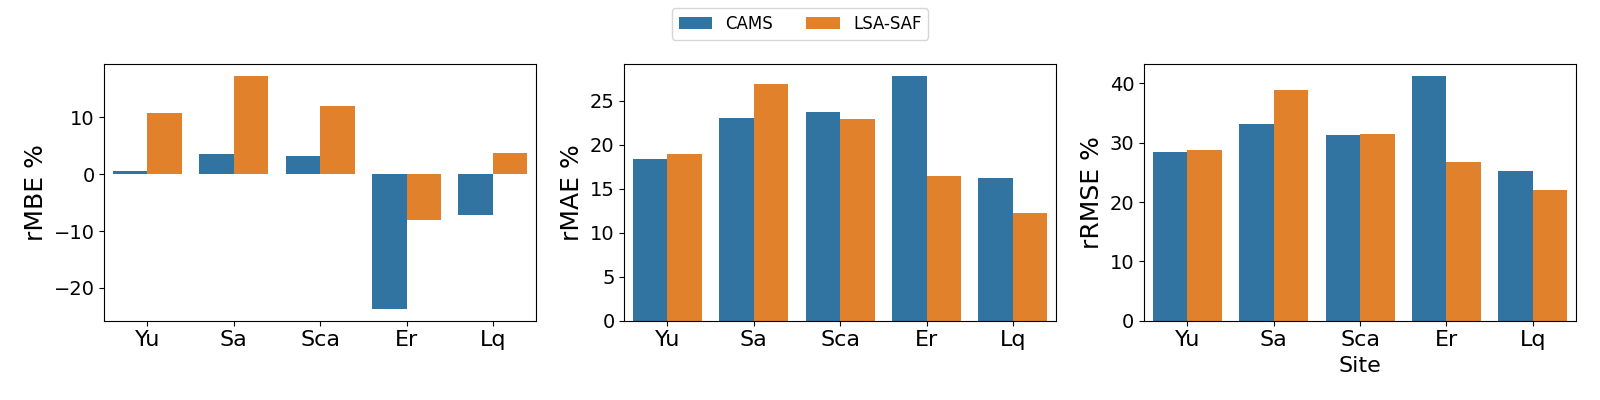
\includegraphics[width=\linewidth]{figuras/errors_15.png}
    \caption{Comparación del desempeño de los modelos CAMS y LSA-SAF en cinco sitios de estudio (Yu, Sa, Sca, Er y Lq) mediante las tres métricas estadísticas: Mean Bias Error (MBE), Mean Absolute Error (MAE) y Root Mean Square Error (RMSE) expresadas en términos relativos a escala 15-minutal.}
    \label{fig:general-15}
\end{figure}

En relación al MAE, ambos modelos presentan magnitudes relativamente similares, aunque LSA-SAF tiende a mostrar errores absolutos ligeramente mayores en sitios como Yu y Sa, mientras que CAMS presenta valores más altos en Sca y Er. Esto sugiere que ninguno de los dos modelos logra una reducción clara y consistente del error en todos los sitios.\\

Por último, en la métrica RMSE, que penaliza los errores grandes, se mantiene un patrón semejante: LSA-SAF suele exhibir errores algo superiores a los de CAMS en Yu y Sa, mientras que en Er y Lq la diferencia favorece al modelo satelital. En general, los resultados muestran que el desempeño relativo de los modelos depende fuertemente del sitio, sin que exista un claro ganador en todos los casos.\\


\begin{figure} 
\centering 
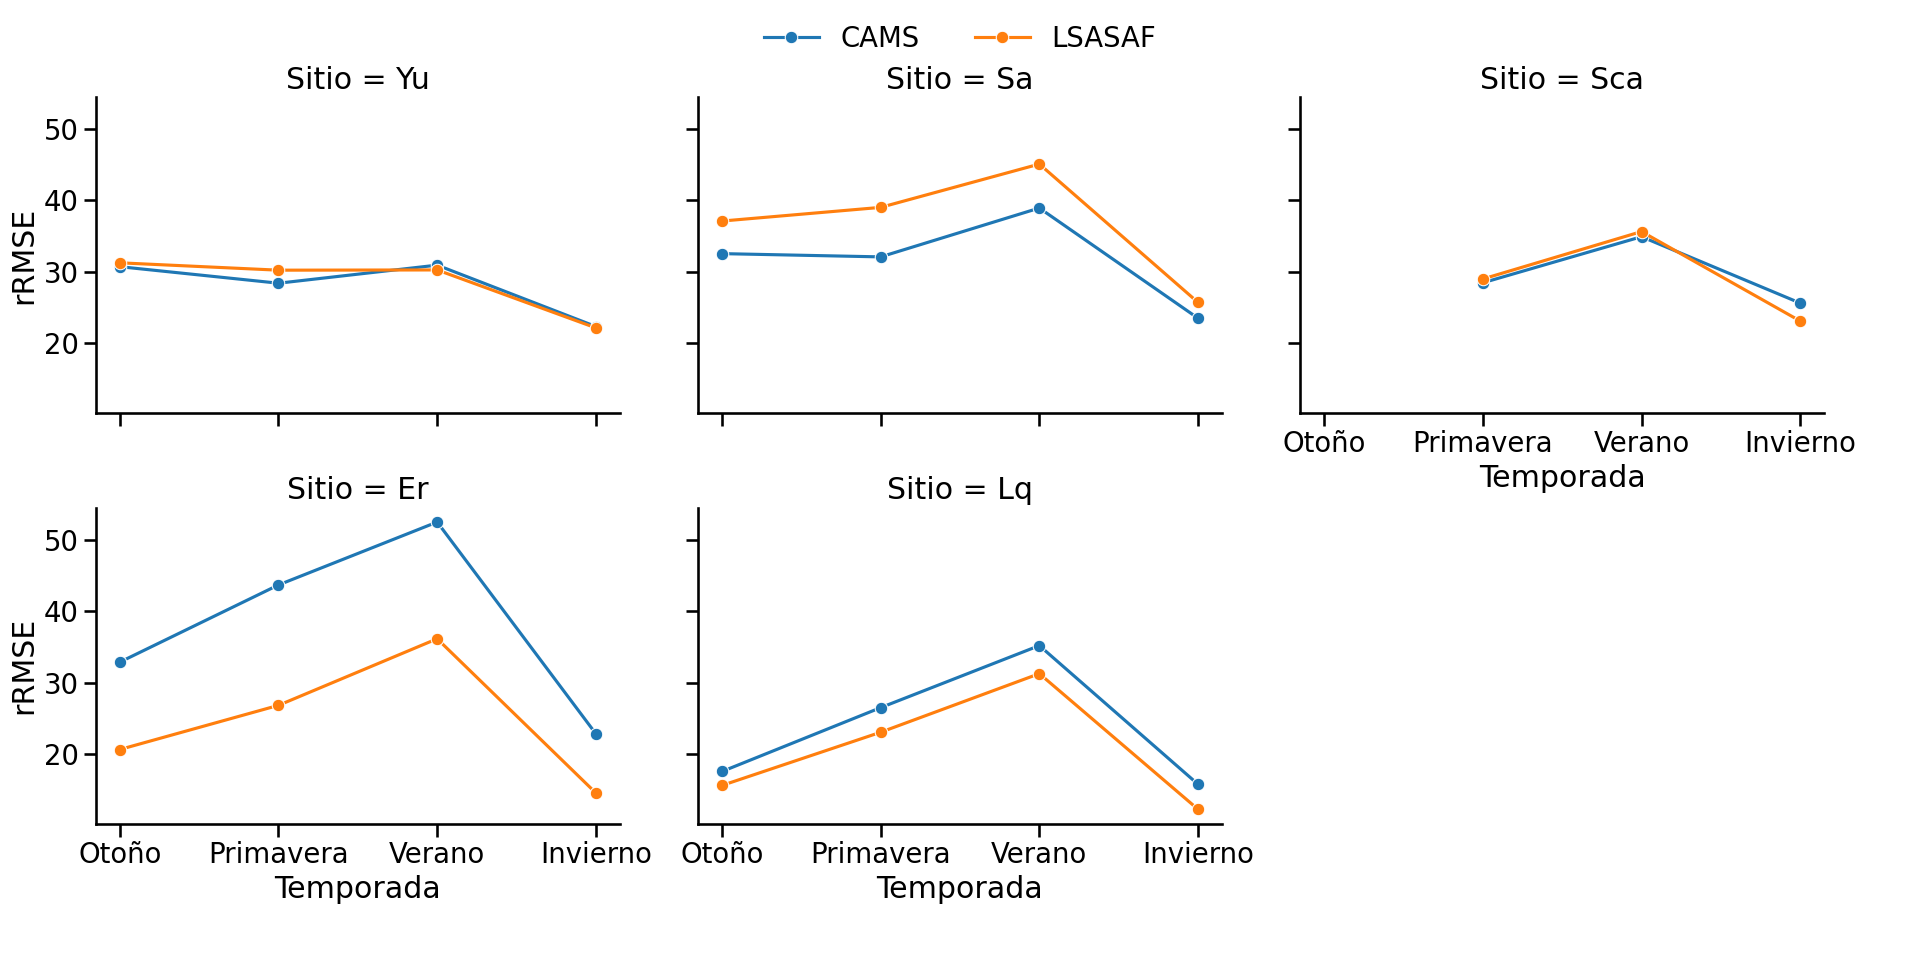
\includegraphics[width=\linewidth]{figuras/season_15_tesis.png}
 \caption{Figura \ref{fig:season-15}. Variación estacional del rRMSE (\%) para los productos CAMS y LSA-SAF con resolución de 15 minutos en todos los sitios de estudio. Se evidencia un aumento del error durante el verano en la mayoría de los sitios, mientras que en Yuto el rRMSE se mantiene estable, sugiriendo que la presencia de nubosidad estacional afecta de manera diferenciada la precisión de las estimaciones de radiación solar.} 
\label{fig:season-15} 
\end{figure}


La Figura \ref{fig:season-15} muestra la variación estacional del rRMSE (\%) para los productos CAMS y LSA-SAF con resolución de 15 minutos en todos los sitios de estudio. Se observa una clara tendencia estacional en el comportamiento del error: en general, el rRMSE tiende a aumentar durante el verano, lo que indica que la precisión de las estimaciones disminuye en este período en la mayoría de los sitios. La excepción es Yuto, donde el error permanece relativamente estable a lo largo de las estaciones. Este patrón sugiere que durante el verano hay una mayor presencia de nubosidad, lo cual podría estar afectando la capacidad de los modelos satelitales para estimar correctamente la radiación solar, mientras que en otras estaciones la cobertura nubosa es menor, permitiendo estimaciones más precisas.







\begin{figure}
    \centering
    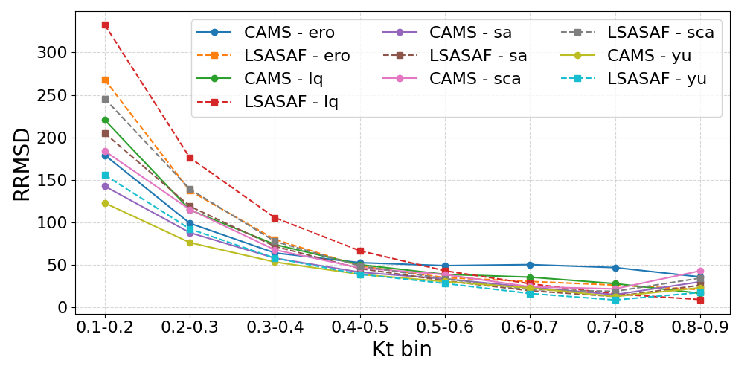
\includegraphics[width=\linewidth]{figuras/RMSE-kt-15.pdf}
    \caption{Variación del error cuadrático medio relativo (RRMSD) en función del indice de claridad (kt) para los cinco sitios analizados (YU, SA, SCA, ERO y LQ). Resultados para CAMS (líneas continuas) y LSASAF (líneas punteadas).}
    \label{fig:RMSE-kt-15}
\end{figure}



En el caso de RRMSD vs Kt (Figura \ref{fig:RMSE-kt-15}), se observa una marcada disminución del error a medida que aumenta la claridad atmosférica. Para condiciones de cielo más nuboso (Kt < 0.3), los valores de RRMSD son elevados en todos los sitios, superando en algunos casos los 200 \%, especialmente en la estimación proveniente de LSASAF. Sin embargo, conforme Kt aumenta (>0.5), el error desciende rápidamente y tiende a estabilizarse por debajo del 50\%, alcanzando valores mínimos en condiciones de cielo despejado (Kt > 0.7). Esta tendencia se mantiene consistente en ambos productos (CAMS y LSASAF), aunque LSASAF presenta errores relativamente mayores en las condiciones más turbias.




\begin{figure}
    \centering
    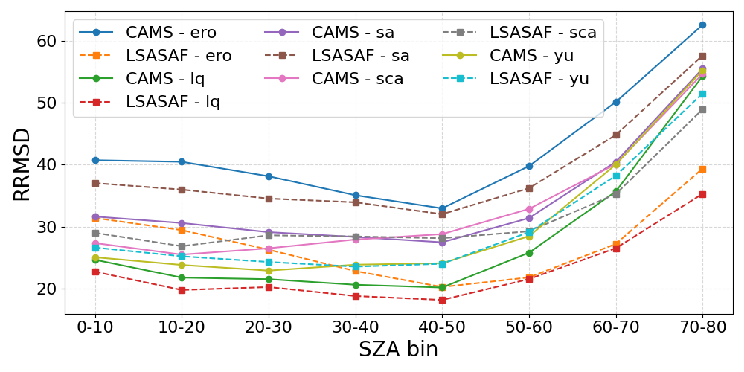
\includegraphics[width=0.8\textwidth]{figuras/RMSE-sza-15.pdf}
    \caption{Variación del error cuadrático medio relativo (RRMSD) en función del ángulo cenital solar (SZA) para los cinco sitios analizados (YU, SA, SCA, ERO y LQ). Resultados para CAMS (líneas continuas) y LSASAF (líneas punteadas).}
    \label{fig:RMSE-SZA-15}
\end{figure}



Por otro lado, la relación RRMSD vs SZA (Figura \ref{fig:RMSE-SZA-15}) evidencia un comportamiento en forma de “U” invertida: los menores errores se concentran en ángulos intermedios (30°–50°), mientras que hacia ángulos bajos (<20°) y altos (>70°) el error aumenta de manera significativa. Esta tendencia se observa en los cinco sitios, con un incremento más pronunciado en ERO y SA en las condiciones de SZA más extremas. En general, CAMS muestra un mejor desempeño que LSASAF en la mayoría de los intervalos, aunque las diferencias se reducen en los ángulos medios.

En conjunto, estos resultados indican que la precisión de ambos productos depende fuertemente de las condiciones atmosféricas (Kt) y de la geometría solar (SZA). En cielos despejados y ángulos intermedios, los errores se reducen notablemente, mientras que en condiciones nubosas y en situaciones de baja o alta elevación solar los modelos presentan las mayores limitaciones.


\subsection{Análisis de las estimaciones horarias}



\subsection{División del conjunto de datos}
De acuerdo a lo indicado en la sección \ref{MLM} el conjunto de datos debe ser segmentado con fin de evaluar el rendimiento de los modelos de aprendizaje automático utilizados en la regresión del proceso de adaptación al sitio y controlar el sobre-entrenamiento de los modelos. En el contexto de AS en los trabajos \cite{POLO2016, POLO2020} se recomienda tomar al menos un año de medidas para la calibración de los modelos. Siguiendo estas ideas el conjunto de medidas fue dividido en subconjunto de entrenamiento, validación y prueba.  


\begin{table}[ht]
    \centering
    \renewcommand{\arraystretch}{1.5} % Espaciado vertical en la tabla
    \begin{tabular}{|>{\centering\arraybackslash}p{2cm}|>{\centering\arraybackslash}p{3cm}|>{\centering\arraybackslash}p{3cm}|>{\centering\arraybackslash}p{4cm}|}
        \hline
        \textbf{ID} & \textbf{Entrenamiento} & \textbf{Validación} & \textbf{Prueba}\\ 
        \hline

        \textbf{YU}  & 2017 & 2017 & 2018 \\ 
        \textbf{SA}  & 2009 & 2009 & 2010 - 2024 \\ 
        \textbf{SCA} & 2013 & 2013 & 2012-2014 \\
        \textbf{ERO} & 2013 & 2013 & 2014 - 2024  \\
        \textbf{LQ}  & 2019 & 2019 & 2018, 2021 - 2023  \\
    \hline
    \end{tabular}
    \caption{División del conjunto de datos en entrenamiento, validación y prueba }
    \label{tab:tvt}
\end{table}

    



\begin{table*}%[]
  \centering
  \label{tbl:metrics_test}
  \caption{Métricas de desempeño (MBE, MAE, RMSE) para cada modelo y conjunto de datos satelitales en los cinco sitios en el \textbf{conjunto de pruebas}. 
           Los valores están normalizados y expresados como porcentajes relativos al promedio de GHI en cada sitio: 
           396.8~W/m$^{2}$ (Yu), 397~W/m$^{2}$ (Sa), 557.1~W/m$^{2}$ (Sca), 690.6~W/m$^{2}$ (Ero) y 673.7~W/m$^{2}$ (Lq).}
  \resizebox{\linewidth}{!}{%
    \begin{tabular}{|l|ccc|ccc|ccc|ccc|ccc|}
      \hline
      & \multicolumn{3}{c|}{YU} & \multicolumn{3}{c|}{SA} & \multicolumn{3}{c|}{SCA} & \multicolumn{3}{c|}{ERO} & \multicolumn{3}{c|}{LQ} \\
      \cline{2-16}
      Modelo  & MBE & MAE & RMSE & MBE & MAE & RMSE & MBE & MAE & RMSE & MBE & MAE & RMSE & MBE & MAE & RMSE \\
      \hline
      \multicolumn{16}{|c|}{\textit{Resolución Temporal: 15 minutos}} \\
      \hline
      CAMS    & -0.2 & 17.4 & 27.2 & 3.9  & 23.4 & 33.7 & 2.6  & 21.8 & 29.8 & -23.6 & 27.6 & 40.9 & -6.9 & 16.5 & 25.8 \\
      LSA-SAF & 7.6  & 16.5 & 25.5 & 17.9 & 27.4 & 39.4 & 13.1 & 22.2 & 30.9 & -7.7  & 16.2 & 26.5 & 4.0  & 12.6 & 22.6 \\
      \hline
      \multicolumn{16}{|c|}{\textit{Resolución Temporal: horaria}} \\
      \hline
      CAMS    & -0.2 & 15.3 & 23.5 & 4.0 & 20.9 & 29.3 & 3.0 & 19.7 & 26.1 & -23.6 & 26.6 & 39.3 & -4.8 & 14.5 & 21.6 \\
      LSA-SAF & 7.6  & 14.5 & 21.9 & 17.9 & 25.3 & 35.7 & 13.3 & 20.3 & 27.1 & -7.7  & 14.8 & 24.0 & 4.8  & 10.9 & 18.2 \\
      ERA-5   & -4.0 & 43.5 & 60.2 & 9.4  & 27.1 & 37.7 & 1.9  & 20.2 & 29.7 & -14.0 & 19.3 & 25.6 & -0.8 & 11.3 & 18.4 \\
      MERRA-2 & 25.0 & 33.6 & 51.2 & 43.4 & 48.3 & 65.0 & 10.9 & 21.7 & 30.3 & -3.8  & 13.1 & 20.4 & 1.4  & 13.4 & 20.8 \\
      \hline
    \end{tabular}%
  }
\end{table*}

    



\section{Adaptación al sitio con una variable descriptiva}\label{sec:01}


En los trabajos citados en la Sección \ref{ch_3} sobre la evaluación del proceso de Adaptación al Sitio (SA), se ha prestado escasa atención a las razones subyacentes por las cuales ciertos modelos de aprendizaje automático (ML) superan a otros en este proceso. Dado que algunos modelos de ML poseen una naturaleza inherentemente más compleja que otros, podría suponerse que los modelos más complejos ofrecerían un rendimiento superior frente a aquellos de menor complejidad. En este contexto, el término complejidad hace referencia tanto a la complejidad computacional —es decir, la cantidad de operaciones necesarias para ejecutar el modelo— como a la complejidad conceptual, relacionada con el nivel de conocimiento requerido para comprender su funcionamiento.\\

En esta sección se presenta una implementación del proceso de SA basada en uno de los enfoques clásicos, que consiste en adaptar una serie temporal modelada (proveniente de datos satelitales o de reanálisis) utilizando como referencia una serie de mediciones in situ.\\

Dado que el modelo de Regresión Lineal Simple (RLS) puede considerarse el menos complejo entre los empleados en este estudio, la primera evaluación del proceso de SA en la región de interés se realiza utilizando este modelo. El objetivo es comparar el desempeño de la RLS con el de modelos de regresión más complejos, como el Perceptrón Multicapa (MLP) y XGBoost, utilizando las mismas métricas de evaluación.\\

Para los modelos MLP y XGBoost, la determinación de la configuración óptima de hiperparámetros fue fundamental para lograr un desempeño consistente en las particiones de validación cruzada. Esto se llevó a cabo mediante una búsqueda exhaustiva en rejilla (Grid Search) implementada con la función \textbf{GridSearchCV} de la biblioteca \textbf{Scikit-learn} en Python \cite{Pedregosa2012}. Los rangos específicos de hiperparámetros evaluados para MLP y XGBoost se presentan en la Tabla \ref{tab:gridsearch}. La selección de hiperparámetros óptimos constituye un paso crítico en el aprendizaje automático, ya que influye directamente en la complejidad del modelo, su capacidad de generalización y su rendimiento predictivo global \cite{Goodfellow2016}.\\



\begin{table}[ht]
\caption{Espacio cartesiano de hiperparámetros para las técnicas de aprendizaje supervisado.}
\label{tab:gridsearch}
\centering
\resizebox{\linewidth}{!} {
\def\arraystretch{1.5}
\begin{tabular}{lcccc}
\hline
\textbf{Hiperparámetro} & \textbf{Inferior} & \textbf{Superior} & \textbf{Paso} & \textbf{Función de transformación} \\
\hline
MLP\\
\hline
 Capas ocultas        & 1    & 3     & 1   & - \\
 Nodos ocultos        & 1    & 4     & 1   & $2^{x}$ \\
 Fracción de dropout  & 0    & 0.3   & 0.1 & - \\
 Tasa de aprendizaje  & -3   & -1    & 1   & $10^{x}$ \\
\hline
XGBoost\\
\hline
Booster               & gbtree & & & \\
 Estimadores          & 1    & 50    & 10  & - \\
 Profundidad máxima   & 2    & 5     & 1   & $2^{x}$ \\
 Tasa de aprendizaje  & -3   & -1    & 1   & $10^{x}$ \\
\hline
\end{tabular}}
\end{table}

En cuanto al preprocesamiento de los datos de entrada, la normalización o el escalado de características es una práctica común en aprendizaje automático para mejorar la convergencia y la estabilidad, particularmente en modelos sensibles a la magnitud de las variables de entrada. Sin embargo, en este estudio \textbf{no se aplicó normalización}, ya que no se consideró necesaria para los modelos y datos utilizados.  

En el caso del modelo \textbf{SLR}, el escalado de la variable independiente no es necesario porque el modelo es inherentemente invariante al escalado: multiplicar la entrada por un factor constante provoca un cambio inversamente proporcional en el coeficiente de la pendiente, dejando las predicciones sin alterar.  

De manera similar, \textbf{XGB}, cuando se implementa con árboles de decisión como aprendices base, \textbf{no requiere escalado de características}, ya que las divisiones en los nodos dependen del \textbf{orden relativo} de los valores y no de sus magnitudes absolutas \cite{Soria2022, Chen2016}.  

En el caso del modelo \textbf{MLP}, el escalado puede ser importante cuando las variables de entrada difieren significativamente en su rango o unidades. Sin embargo, en el presente estudio se utilizó \textbf{una sola variable de entrada} (GHI derivado de satélite), expresada en las \textbf{mismas unidades y rango} que la variable objetivo (GHI medido en superficie). Por lo tanto, no se consideró necesaria ninguna normalización adicional.

Los resultados obtenidos son expresados en la Tabla \ref{tab:metrics-as-1}.


\begin{table*}%[]
  \centering
  \label{tab:metrics-as-1}
  \caption{Métricas de desempeño (MBE, MAE, RMSE) para cada modelo adaptado en los cinco sitios en el \textbf{conjunto de pruebas}}
  \resizebox{\linewidth}{!}{%
    \begin{tabular}{|l|ccc|ccc|ccc|ccc|ccc|}
      \hline
      & \multicolumn{3}{c|}{YU} & \multicolumn{3}{c|}{SA} & \multicolumn{3}{c|}{SCA} & \multicolumn{3}{c|}{ERO} & \multicolumn{3}{c|}{LQ} \\
      \cline{2-16}
      Modelo  & MBE & MAE & RMSE & MBE & MAE & RMSE & MBE & MAE & RMSE & MBE & MAE & RMSE & MBE & MAE & RMSE \\
      \hline
      \multicolumn{16}{|c|}{\textit{Resolución Temporal: 15 minutos}} \\
      \hline
      CAMS SLR    & -0.9 & 17.1 & 26.4 &  3.8 & 21.3 & 31.5 & -1.5 & 18.4 & 26.0 &  2.5 & 24.8 & 31.5 &  2.1 & 15.9 & 23.5 \\
      CAMS MLP    & -4.4 & 17.7 & 26.2 &  4.8 & 21.4 & 31.6 &  7.7 & 17.8 & 27.7 &  0.5 & 24.1 & 31.2 &  9.1 & 19.4 & 25.6 \\
      CAMS XGB    & -1.3 & 17.1 & 26.0 &  3.8 & 21.4 & 31.4 & -1.8 & 18.9 & 26.2 &  2.5 & 23.9 & 30.9 &  2.2 & 15.9 & 23.5 \\
      \hline
      LSASAF SLR  & -5.5 & 18.4 & 25.0 &  4.4 & 23.9 & 34.6 &  1.0 & 18.0 & 26.7 &  2.7 & 17.1 & 25.4 &  2.2 & 12.9 & 22.3 \\
      LSASAF MLP  & -7.1 & 18.6 & 25.0 &  4.5 & 23.6 & 34.5 &  5.9 & 18.4 & 26.6 &  2.5 & 17.0 & 25.3 & -0.4 & 13.6 & 22.1 \\    
      LSASAF XGB  & -6.0 & 18.2 & 24.9 &  4.3 & 23.9 & 34.6 &  0.5 & 18.6 & 27.0 &  2.4 & 17.2 & 25.1 &  2.3 & 13.1 & 22.3 \\
      \hline
      \multicolumn{16}{|c|}{\textit{Resolución Temporal: horaria}} \\
      \hline
      CAMS SLR    & -1.3 & 14.7 & 22.7 &  3.5 & 18.5 & 27.0 & -1.7 & 15.9 & 22.0 &  2.1 & 23.4 & 29.6 &  2.6 & 13.8 & 19.4 \\
      LSASAF SLR  & -5.5 & 16.0 & 21.2 &  4.3 & 21.2 & 30.5 &  1.1 & 15.6 & 22.7 &  2.5 & 15.7 & 22.8 &  0.3 & 10.6 & 17.4 \\
      ERA-5 SLR   &  1.2 & 44.0 & 55.1 &  6.4 & 26.5 & 36.9 & -6.4 & 20.1 & 29.1 & -0.6 & 15.4 & 21.4 &  2.1 & 11.6 & 18.4 \\
      MERRA-2 SLR & -3.6 & 34.7 & 44.1 &  7.1 & 35.2 & 46.0 & -2.2 & 20.3 & 27.7 &  0.7 & 12.9 & 20.1 &  0.3 & 13.1 & 20.4 \\
      \hline
      CAMS MLP    & -4.9 & 16.2 & 23.0 &  4.3 & 18.6 & 27.2 & -4.0 & 16.6 & 22.4 &  3.8 & 23.5 & 29.5 & -0.5 & 13.0 & 19.2 \\
      LSASAF MLP  & -5.4 & 15.4 & 20.9 &  2.5 & 21.4 & 30.2 &  8.3 & 16.1 & 24.1 &  9.6 & 19.4 & 24.6 & -3.8 & 12.1 & 17.8 \\
      ERA-5 MLP   &  0.2 & 43.7 & 55.1 &  9.6 & 27.1 & 37.6 & -1.8 & 19.0 & 28.5 & -7.5 & 16.7 & 23.1 &  0.1 & 11.3 & 18.3 \\
      MERRA-2 MLP &  0.7 & 33.7 & 43.9 &  0.8 & 36.3 & 45.4 & -0.3 & 19.5 & 27.5 & 11.7 & 17.5 & 23.4 & -2.8 & 13.4 & 20.6 \\
      \hline
      CAMS XGB    & -1.6 & 14.8 & 22.2 &  3.4 & 18.9 & 27.1 & -2.4 & 16.6 & 22.4 &  2.1 & 22.8 & 29.2 &  2.7 & 13.9 & 19.6 \\
      LSASAF XGB  & -6.1 & 16.0 & 21.3 &  4.1 & 21.4 & 30.6 &  0.0 & 16.9 & 23.4 &  2.2 & 15.9 & 22.6 &  0.2 & 10.9 & 17.4 \\
      ERA-5 XGB   &  1.4 & 44.6 & 55.4 &  6.3 & 27.3 & 37.4 & -7.3 & 20.7 & 29.3 & -0.5 & 15.2 & 21.2 &  2.0 & 11.8 & 18.6 \\
      MERRA-2 XGB & -4.9 & 35.3 & 44.5 &  6.9 & 35.6 & 46.1 & -2.8 & 20.8 & 28.2 &  0.8 & 13.3 & 20.3 &  0.2 & 13.5 & 20.6 \\
      \hline
    \end{tabular}%
  }
\end{table*}

La evaluación comparativa de los modelos SLR,MLP y XGB, utilizando como variables de entrada los productos satelitales \textit{CAMS} y \textit{LSA-SAF}, se realizó en cinco sitios con características climáticas y geográficas diversas. El desempeño se expresó en términos de error medio de sesgo (MBE), error absoluto medio (MAE) y raíz del error cuadrático medio (RMSE), todos normalizados respecto al promedio de la irradiancia global horizontal (GHI) en cada estación (Tablas~\ref{tab:metrics-as-1} y \ref{tbl:metrics_test}).  

En términos generales, los errores normalizados se mantuvieron dentro de un rango moderado en todas las combinaciones de modelos y conjuntos de datos, sin observarse diferencias sustanciales entre los enfoques lineales y los no lineales. El modelo RLS mostró un desempeño competitivo en ambos conjuntos de datos, con métricas de error cercanas a las obtenidas por los modelos más complejos.  

En el caso de \textbf{CAMS}, aunque el MLP logró reducir ligeramente el RMSE en algunos sitios, esto se produjo a costa de sesgos más pronunciados en el MBE, lo cual evidencia una compensación entre reducción de varianza e incremento del error sistemático. El modelo XGB, por su parte, presentó un comportamiento muy similar al de RLS, con diferencias marginales.  

Por otro lado, al emplear \textbf{LSA-SAF} se observó una ligera mejora respecto a CAMS, particularmente en estaciones de mayor altitud (ERO y LQ), donde tanto XGB como MLP alcanzaron menores valores de MAE y RMSE. Esto sugiere que la mayor resolución temporal o la representación más detallada de nubes en LSA-SAF aportan información adicional útil para el proceso de adaptación local.  

No obstante, el incremento de la complejidad del modelo no se tradujo en ganancias sustanciales de desempeño. Estos resultados indican que, dadas las condiciones actuales de calidad de los datos satelitales, los modelos simples como RLS son capaces de capturar gran parte de la relación entre los insumos derivados de satélite y las mediciones de GHI en superficie, ofreciendo además mayor robustez frente al ruido y a las limitaciones en los datos de entrenamiento.  

\begin{figure}[ht]
\centering
\begin{tikzpicture}
\begin{axis}[
    ybar,
    bar width=7pt,
    width=\linewidth,
    height=8cm,
    ylabel={RMSE [\%]},
    xlabel={Sitios},
    symbolic x coords={YU, SA, SCA, ERO, LQ},
    xtick=data,
    xticklabel style={rotate=45, anchor=east},
    enlarge x limits=0.1,
    ymin=0,
    nodes near coords,
    nodes near coords style={font=\scriptsize, rotate=90, anchor=west, text=black!85},
    legend style={at={(0.5,-0.30)}, anchor=north, legend columns=4, font=\small},
    cycle list={{blue!70},{blue!40},{cyan!60},{green!60},{red!70},{red!40},{orange!60},{purple!60}}
]

% ---- CAMS sin adaptar ----
\addplot+[fill=blue!70] coordinates {(YU,27.2) (SA,33.7) (SCA,29.8) (ERO,40.9) (LQ,25.8)};

% ---- CAMS adaptados ----
\addplot+[fill=blue!40] coordinates {(YU,26.4) (SA,31.5) (SCA,26.0) (ERO,31.5) (LQ,23.5)}; % SLR
\addplot+[fill=cyan!60] coordinates {(YU,26.2) (SA,31.6) (SCA,27.7) (ERO,31.2) (LQ,25.6)}; % MLP
\addplot+[fill=green!60] coordinates {(YU,26.0) (SA,31.4) (SCA,26.2) (ERO,30.9) (LQ,23.5)}; % XGB

% ---- LSA-SAF sin adaptar ----
\addplot+[fill=red!70] coordinates {(YU,25.5) (SA,39.4) (SCA,30.9) (ERO,26.5) (LQ,22.6)};

% ---- LSA-SAF adaptados ----
\addplot+[fill=red!40] coordinates {(YU,25.0) (SA,34.6) (SCA,26.7) (ERO,25.4) (LQ,22.3)}; % SLR
\addplot+[fill=orange!60] coordinates {(YU,25.0) (SA,34.5) (SCA,26.6) (ERO,25.3) (LQ,22.1)}; % MLP
\addplot+[fill=purple!60] coordinates {(YU,24.9) (SA,34.6) (SCA,27.0) (ERO,25.1) (LQ,22.3)}; % XGB

\legend{CAMS (sin adaptar), CAMS SLR, CAMS MLP, CAMS XGB, 
        LSA-SAF (sin adaptar), LSA-SAF SLR, LSA-SAF MLP, LSA-SAF XGB}
\end{axis}
\end{tikzpicture}
\caption{RMSE en resolución de 15 minutos para cada modelo y sitio, comparando modelos sin adaptación y adaptados.}
\label{fig:rmse15}
\end{figure}

La Figura \ref{fig:rmse15} muestra el comportamiento del RMSE (\%) en cada sitio para los diferentes modelos de regresión utilizados. Se observa que todas las propuestas de adaptación logran reducir el RMSE en cada sitio. Aunque en algunos casos la mejora puede ser modesta, como en YU y LQ, queda evidenciado que un simple ajuste específico puede mejorar el desempeño del modelo para una ubicación determinada. Además se puede apreciar que el grado de mejora mediante la adaptación aparenta depender del modelo de estimación empleado. Cada modelo impone un límite sobre la precisión de la serie resultante, y optimizar su salida no garantiza necesariamente un desempeño superior frente a otro modelo que, de forma natural, ya proporciona una estimación más adecuada para un sitio específico.\\




\begin{figure}
    \centering
    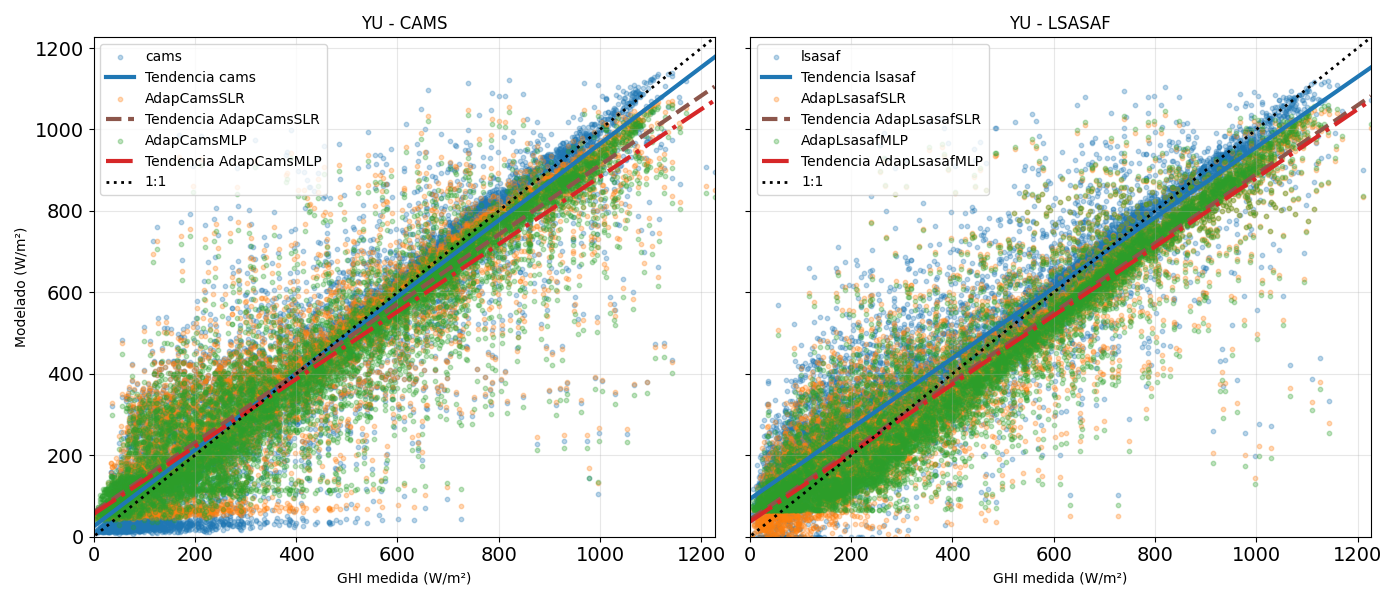
\includegraphics[width=0.9\textwidth]{figuras/scatter_yu_1.png}
    \caption{Comparación de modelos CAMS y LSASAF y las adpaciones con SLR y MLP en Yuto.}
    \label{fig:scatter-yu-01}
\end{figure}


La Figura \ref{fig:scatter-yu-01} muestra un gráfico de dispersión para la GHI medida y las los modelos de CAMS (izquierdo) y LSA-SAF (derecho) con sus correspondeintes adaptaciones usando SLR y MLP.   


\begin{figure}
    \centering
    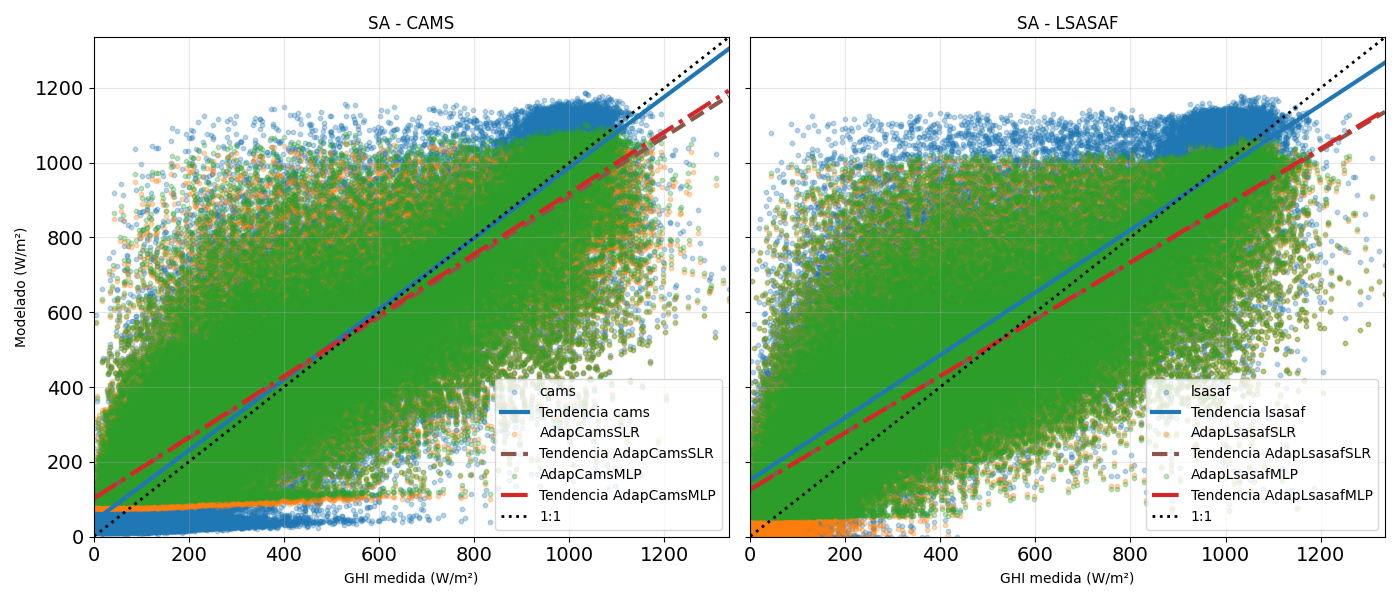
\includegraphics[width=0.9\textwidth]{figuras/scatter_sa_1.png}
    \caption{Comparación de modelos CAMS y LSASAF y las adaptaciones con SLR Y MLP en Salta.}
    \label{fig:scatter-sa-01}
\end{figure}


\begin{figure}
    \centering
    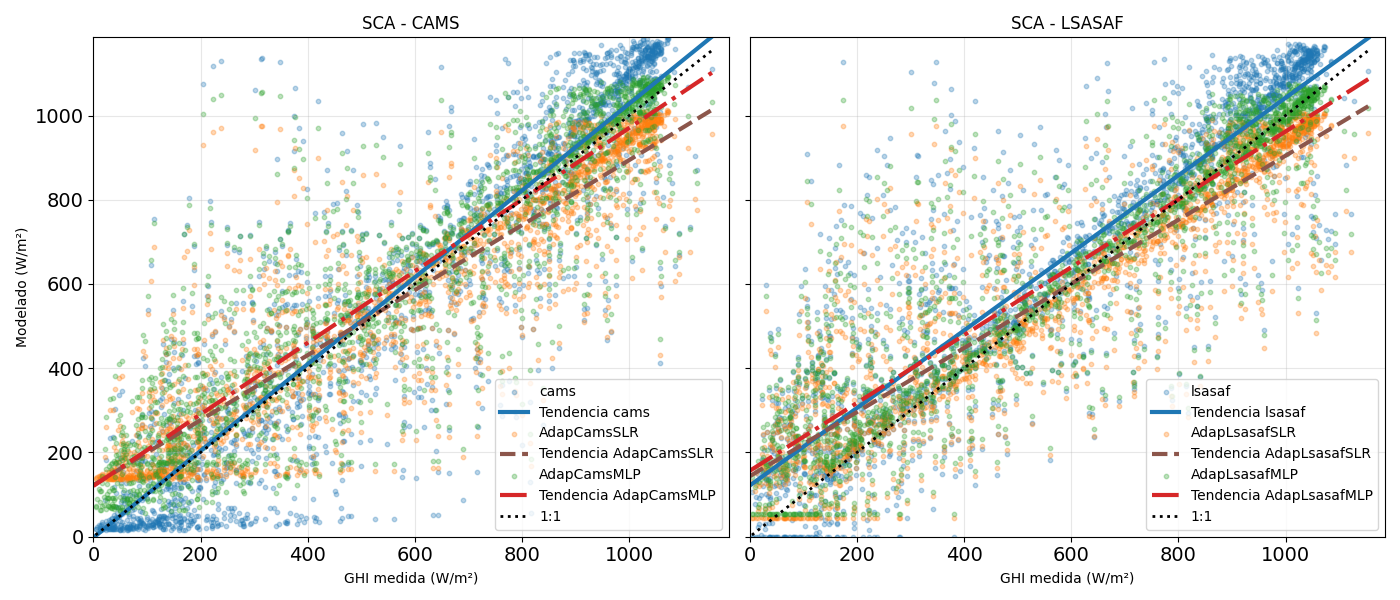
\includegraphics[width=0.9\textwidth]{figuras/scatter_sca_1.png}
    \caption{Comparación de modelos CAMS y LSASAF y las adpataciones con SLR y MLP en San Carlos.}
    \label{fig:scatter-sca-01}
\end{figure}


\begin{figure}
    \centering
    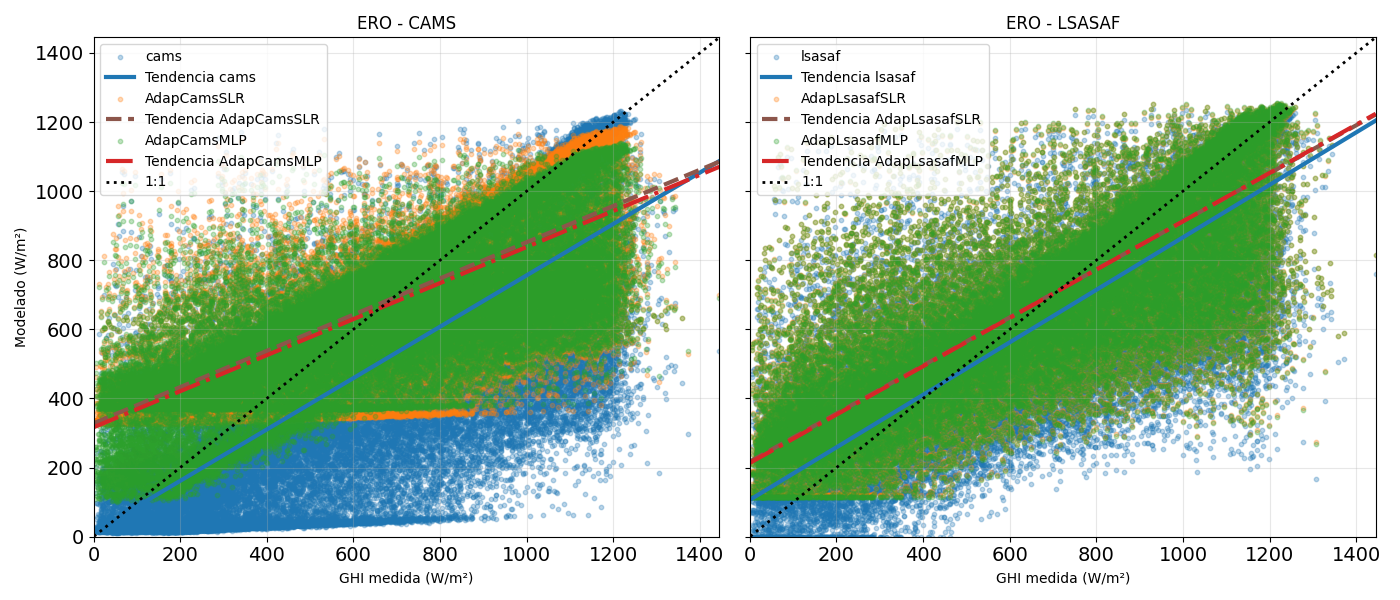
\includegraphics[width=0.9\textwidth]{figuras/scatter_ero_1.png}
    \caption{Comparación de modelos CAMS y LSASAF y las adaptaciones con SLR y MLP en El Rosal.}
    \label{fig:scatter-ero-01}
\end{figure}



\begin{figure}
    \centering
    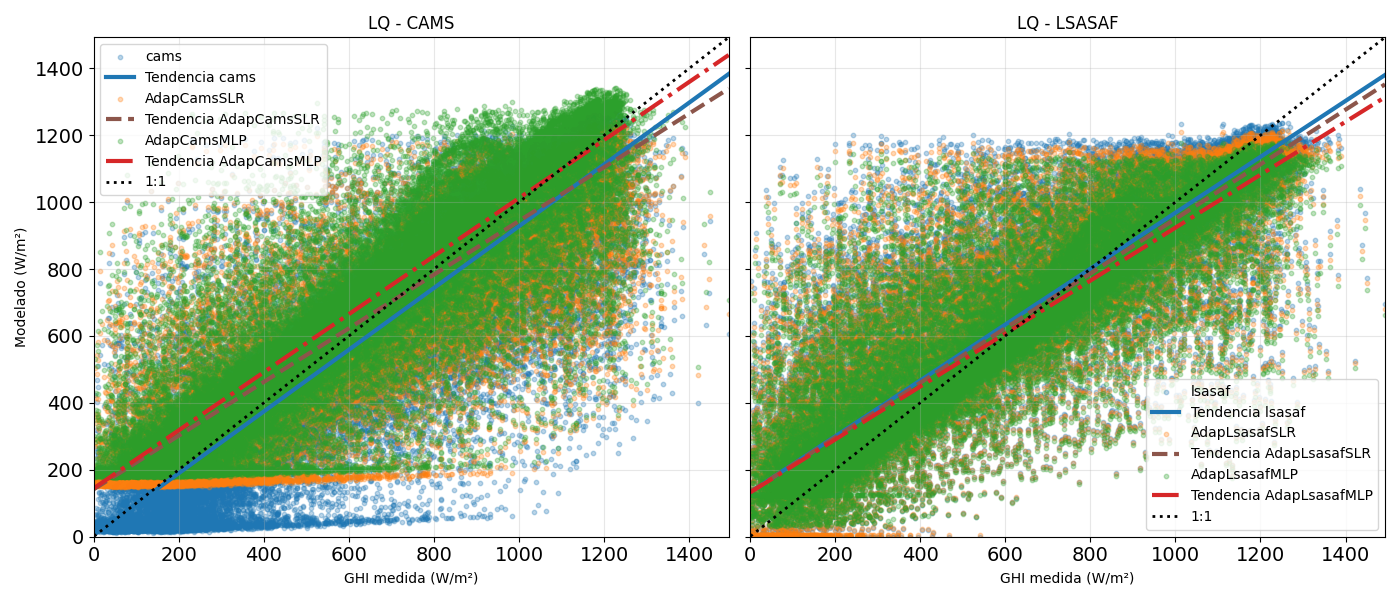
\includegraphics[width=0.9\textwidth]{figuras/scatter_lq_1.png}
    \caption{Comparación de modelos CAMS y LSASAF y las adaptaciones con SLR y MLP en La Quiaca.}
    \label{fig:scatter-lq-01}
\end{figure}



La Figura \ref{fig:mejorModelo} presenta las variaciones del rRMSE en cada sitio considerando el mejor desemepeño obtenido (menor rRMSE). Puede notarse que las ganancias sobre el desempeño podrían considerarse marginales, sin embargo sería interesante considerar el impacto que podria tener una variación del 3\% en la estimación del recurso solar, por ejemplo en la aplicación práctica.\\
\begin{figure}
    \centering
    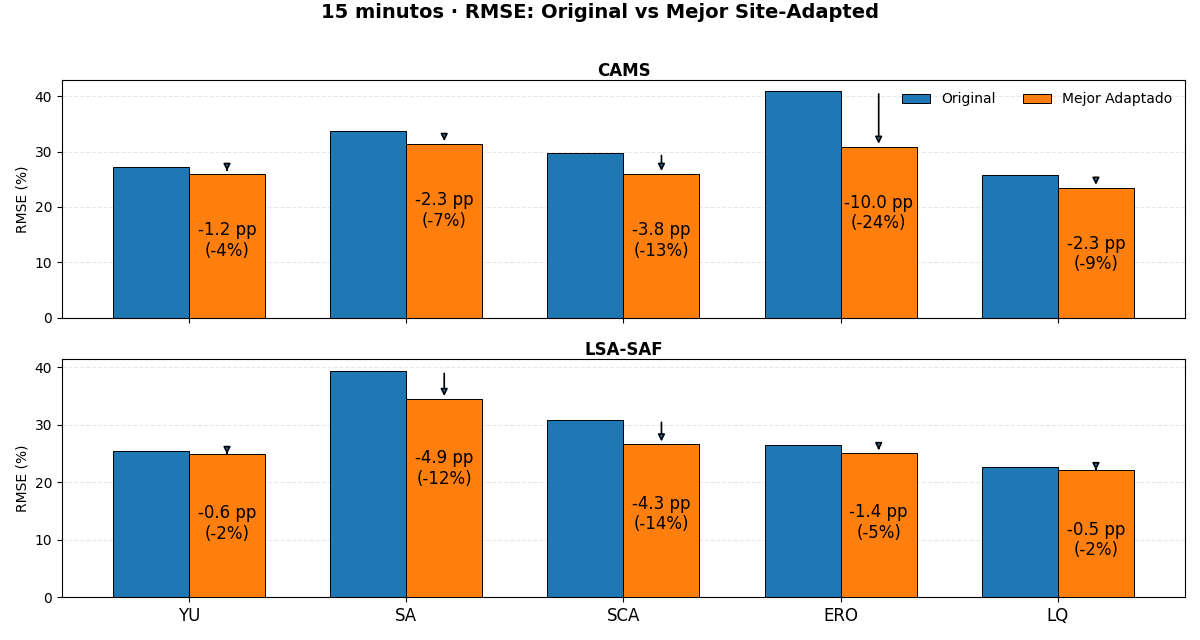
\includegraphics[width=0.9\textwidth]{figuras/comparativasRMSE15.png}
    \caption{Comparación del RMSE(\%) para los modelos crudos y el mejor desempeño obtenido.}
    \label{fig:mejorModelo}
\end{figure}





%\begin{figure}
%    \centering
%    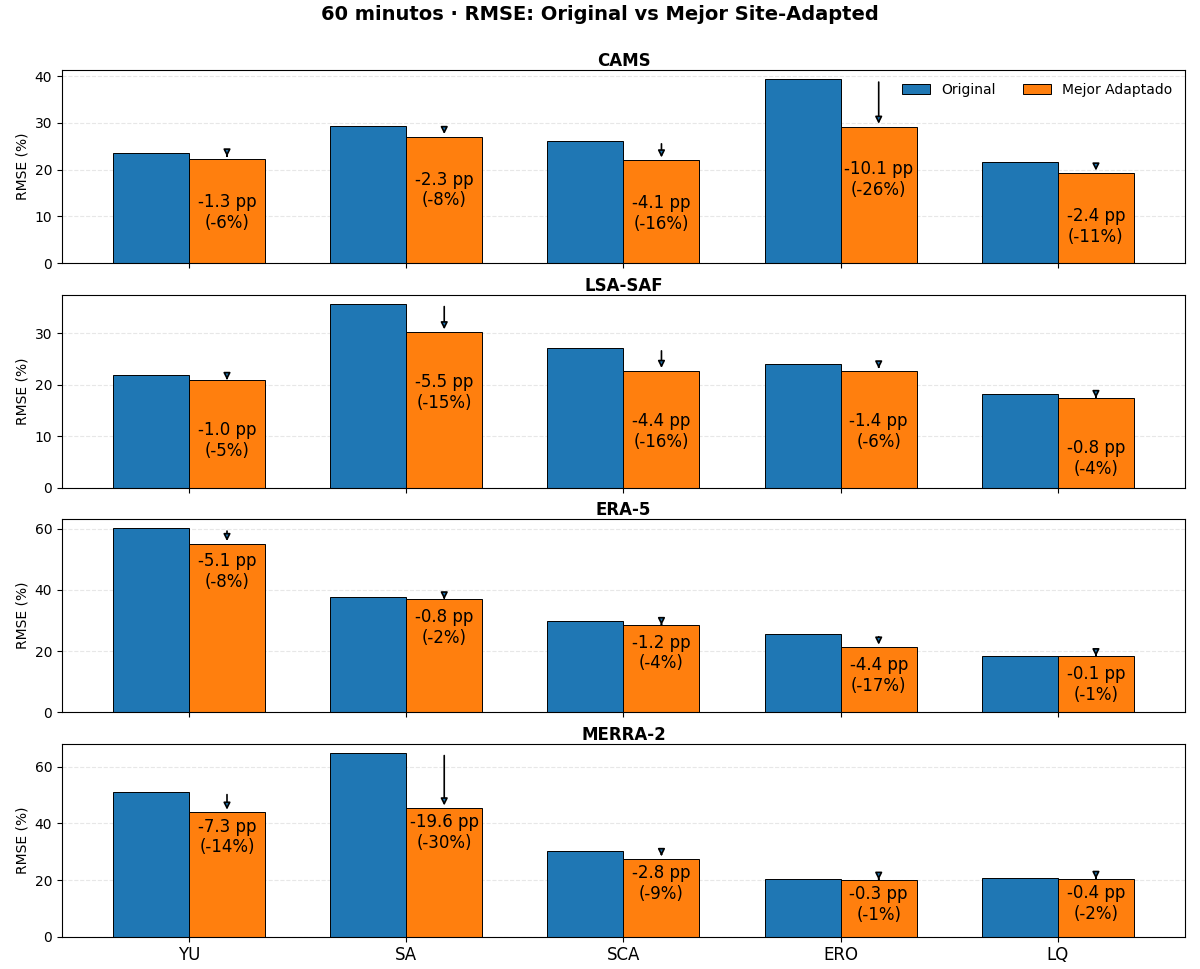
\includegraphics[width=0.9\textwidth]{figuras/comparativasRMSE60.png}
%    \caption{Variación del error cuadrático medio relativo (RRMSD) en función del ángulo cenital solar (SZA) para los cinco sitios analizados (YU, SA, SCA, ERO y LQ). Resultados para CAMS (líneas continuas) y LSASAF (líneas punteadas).}
%    \label{fig:RMSE-60}
%\end{figure}


Los hallazgos de este primer estudio indican que, en el contexto de la adaptación del sitio para GHI utilizando productos derivados de satélite como CAMS y LSA-SAF, los modelos de aprendizaje automático evaluados SLR, XGB y MLP mostraron un rendimiento comparable en términos de métricas de error estándar, con diferencias mínimas entre ellos. A pesar de su simplicidad, SLR demostró una notable capacidad para capturar la relación entre los datos derivados de satélite y las mediciones terrestres, logrando niveles de error relativo similares a los obtenidos por los modelos XGB y MLP, más complejos.
Estos resultados sugieren que la calidad de los datos de entrada impone un límite superior a las mejoras de precisión alcanzables que ofrecen los modelos complejos. Los productos satelitales empleados presentan incertidumbres inherentes y carecen de la resolución necesaria para considerar fenómenos localizados de alta frecuencia, como los efectos microclimáticos o la variabilidad inducida por el terreno. En consecuencia, aumentar la complejidad del modelo no mejora sustancialmente el rendimiento predictivo en estas condiciones de datos. En este sentido, la capacidad predictiva de los modelos complejos se vuelve redundante cuando la relación subyacente entre las variables es predominantemente lineal o solo ligeramente no lineal, lo que explica el excelente rendimiento del SLR.
Además, el análisis reveló que los modelos más flexibles, como el MLP, son propensos al sobreajuste, lo que genera un comportamiento inconsistente en diferentes métricas de rendimiento. Esto subraya la importancia de equilibrar la complejidad del modelo con la calidad de los datos para evitar comprometer la capacidad de generalización del modelo. En resumen, dada la calidad actual de los datos y las características del sitio, modelos simples como el SLR representan una solución robusta, interpretable y computacionalmente eficiente para la estimación del GHI adaptada al sitio. Es más probable lograr mejoras significativas en la precisión de la estimación incorporando variables meteorológicas adicionales, aplicando técnicas de descomposición temporal o desarrollando enfoques híbridos que combinen modelos físicos con correcciones estadísticas, en lugar de simplemente aumentar la complejidad de los algoritmos de aprendizaje automático.

 


\section{Adaptación al sitio con múltiples variables descriptivas}\label{sec:02}
En la sección anterior se presentaron los resultados del proceso de Adaptación al Sitio (SA) utilizando un enfoque basado en mejorar la estimación de un modelo a partir de la variable propiamente modelada y de mediciones in situ. Este enfoque tradicional se centra en la relación directa entre la variable objetivo y sus observaciones, pero en los últimos años se ha desarrollado una estrategia más avanzada que consiste en incorporar variables regresoras adicionales durante el entrenamiento de los modelos de regresión. La idea subyacente es que estas variables pueden aportar información complementaria, lo que podría mejorar la precisión de la estimación en comparación con un enfoque que utiliza únicamente una variable regresora. 

En la práctica, estas variables adicionales pueden provenir de distintos modelos de reanálisis o de fuentes satelitales, y se seleccionan con la expectativa de que estén correlacionadas, de alguna manera, con la irradiancia global horizontal (GHI) medida. Este enfoque ha sido aplicado y documentado en trabajos previos, como \cite{Salazar2025, Miranda2021, Miranda2023}.\\

La idea de ampliar el conjunto de regresores y automatizar el proceso de entrenamiento con la expectativa de obtener mejores resultados resulta atractiva, especialmente considerando que los modelos de aprendizaje automático son cada vez más utilizados para identificar patrones y extraer información de grandes volúmenes de datos. Sin embargo, la efectividad de estos modelos depende en gran medida de la calidad y relevancia de los regresores empleados. No basta con añadir más variables; estas deben ser apropiadas y contener información útil para la tarea de predicción.\\

En este contexto, la \textbf{selección de características} se convierte en un paso crítico del preprocesamiento de datos. Este proceso consiste en identificar las variables más relevantes y eliminar aquellas redundantes o irrelevantes \cite{liu2023, Huang2024}. La selección adecuada de características no solo incrementa la interpretabilidad del modelo, sino que también mejora su eficiencia computacional y su capacidad predictiva. Por el contrario, la inclusión de un exceso de variables o de regresores irrelevantes puede generar sobreajuste, donde el modelo muestra un buen desempeño en los datos de entrenamiento pero falla al generalizar a datos no vistos \cite{che2024a}. Al reducir la dimensionalidad y centrarse en las características más informativas, la selección de características fomenta la creación de modelos más robustos y generalizables, al tiempo que disminuye los costos computacionales y el tiempo requerido para entrenar el modelo, consolidándose como una herramienta esencial tanto para investigadores como para profesionales \cite{Cheng2024}.



Las técnicas de selección de características se agrupan en tres categorías principales: \textbf{métodos de filtro, métodos envolventes y métodos embebidos}, cada uno con su propia metodología, ventajas y limitaciones:  

\paragraph{Métodos de filtro.} Los métodos de filtro evalúan la relevancia de cada característica mediante criterios estadísticos como correlación, información mutua o varianza. Son computacionalmente eficientes y no dependen de un algoritmo de aprendizaje específico. Sin embargo, pueden no captar las interacciones entre variables. Ejemplos comunes incluyen la correlación de Pearson, las pruebas chi-cuadrado y la ganancia de información.  

\paragraph{Métodos envolventes.} Estos métodos consisten en entrenar y evaluar un modelo de aprendizaje automático múltiples veces para identificar el subconjunto óptimo de características. Técnicas como la selección hacia adelante, la eliminación hacia atrás y la eliminación recursiva de características (RFE) son ejemplos típicos \cite{Che2024b,liu2024}. Aunque suelen proporcionar mayor precisión, son costosos en términos computacionales y pueden no escalar eficientemente con conjuntos de datos grandes.  

\paragraph{Métodos embebidos.} Los métodos embebidos incorporan la selección de características directamente en el proceso de entrenamiento del modelo. Ejemplos incluyen técnicas de regularización como LASSO (regularización L1) y modelos basados en árboles de decisión. Este enfoque logra un equilibrio entre eficiencia y rendimiento, convirtiéndolo en una opción ampliamente utilizada en distintas aplicaciones. \\

Comprender estas técnicas permite a los profesionales seleccionar el método más adecuado según las características del conjunto de datos, el dominio del problema y las limitaciones computacionales.\\

En esta sección se documentan los resultados obtenidos al seleccionar tres métodos complementarios para la selección de variables con el objetivo de identificar los mejores regresores que contribuyan a la mejora de la estimación de la GHI en el contexto de la adaptación al sitio: RFE, LASSO y Stepwise.  

\paragraph{Eliminación recursiva de características (RFE).} RFE permite evaluar de manera iterativa la importancia de cada variable en el modelo, eliminando progresivamente las menos relevantes. Este enfoque es particularmente útil en el análisis de variables de geometría solar, donde pueden existir correlaciones complejas entre diferentes parámetros. Al utilizar RFE, se asegura que las variables seleccionadas aporten información significativa al modelo y reduzcan el riesgo de sobreajuste.  

\paragraph{LASSO (Least Absolute Shrinkage and Selection Operator).} LASSO integra la selección de variables en el propio proceso de entrenamiento mediante regularización L1. Este método penaliza los coeficientes de variables menos relevantes, promoviendo modelos más simples y generalizables. La utilización de LASSO en nuestro estudio permite manejar de manera eficiente la multicolinealidad entre parámetros solares y resaltar únicamente los regresores que contribuyen de manera significativa a la predicción de la GHI.  

\paragraph{Stepwise (selección hacia adelante y hacia atrás).} Los métodos Stepwise combinan criterios estadísticos de inclusión y exclusión de variables, permitiendo construir un modelo óptimo de manera secuencial. Este enfoque es especialmente adecuado cuando se busca un balance entre interpretabilidad y rendimiento predictivo. En el contexto de variables solares, Stepwise ayuda a identificar combinaciones de regresores que optimizan la estimación de la GHI sin introducir redundancias innecesarias. \\ 


La elección de los tres métodos de selección de variables se justifica por su complementariedad: RFE se centra en la importancia iterativa de cada predictor, LASSO introduce regularización para reducir la complejidad, y Stepwise optimiza la construcción del modelo desde un enfoque estadístico. Pretendemos que la combinación de estas técnicas permita una selección robusta de variables, maximizando la eficiencia del modelo.\\

En este trabajo el se propuso utilizar un conjunto de variables de carácter astronómico, atmosférico, satelital y meteorológico, definidas de la siguiente manera:

\begin{itemize}
\item \texttt{SZA}: Ángulo cenital solar.
\item \texttt{$\alpha$}: Altura solar.
\item \texttt{TOA}: Irradiancia en la parte superior de la atmósfera.
\item \texttt{GHIargp2}: Irradiancia bajo cielo despejado basada en \cite{Ledesma2023a}.
\item \texttt{delta}: Declinación solar.
\item \texttt{Fn}: Función normalizada de duración del día.
\item \texttt{E0}: Factor de corrección extraterrestre.
\item \texttt{mr}: Masa de aire relativa \cite{Gueymard2003}.
\item \texttt{kt}: Índice de claridad.
\item \texttt{tm}: Temperatura media del aire según ERA-5.
\item \texttt{uw}: Componente U del viento según ERA-5.
\item \texttt{dw}: Componente V del viento según ERA-5.
\item \texttt{hr}: Humedad relativa según ERA-5.
\item \texttt{p}: Presión según ERA-5.
\end{itemize}


\begin{figure}
    \centering
    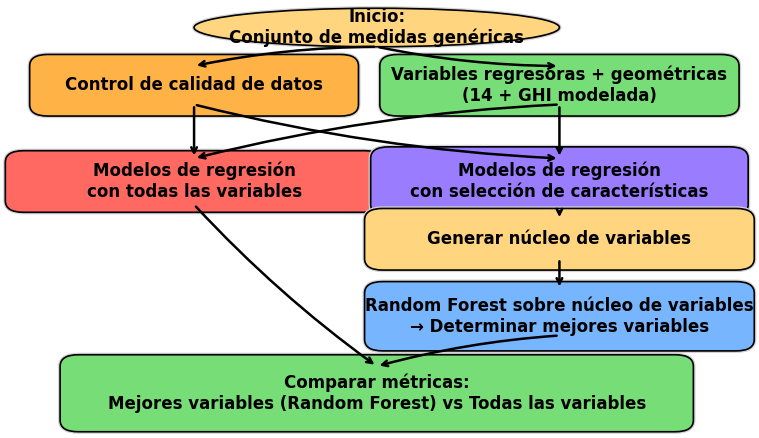
\includegraphics[width=0.65\textwidth]{figuras/procedure_1.png}
    \caption{Flujo de procesamiento para la adaptación de GHI en un sitio. A partir de un conjunto de medida, los datos pasan por un control de calidad y en paralelo se obtienen variables regresoras de reanálisis y geométricas. Con estas se entrenan modelos de regresión en dos enfoques: usando todas las variables disponibles o aplicando selección de características. El segundo enfoque genera un núcleo de variables que es refinado con Random Forest para identificar las más relevantes. Finalmente, se comparan las métricas de desempeño entre los modelos construidos con todas las variables y aquellos basados en las variables óptimas.}
    \label{fig:procedureSA01}
\end{figure}



Las métricas de desempeño obtenidas sobre las series generadas a partir del conjunto completo de variables regresoras se reporta en la Tabla \ref{tab:metricas_3_1}. Además se han incluido, para comidad del lector, nuevamente las métricas obtenidas en partir de la adaptación con una ùnica variable y sin adaptar.

\begin{table*}
\caption{Métricas de desempeño (MBE, MAE, RMSE) para cada modelo en el conjunto de prubeas de los cinco sitios. Los valores están normalizados y expresados como porcentajes relativos a la media de GHI en cada sitio: 429.2~W/m$^2$ (Yu), 432.9~W/m$^2$ (Sa), 554.4~W/m$^2$ (Sca), 628.4~W/m$^2$ (Ero), y 648.7~W/m$^2$ (Lq). Los modelos etiquetados con ``(1 var.)'' indican adaptación al sitio realizada utilizando solo un regresor (CAMS o LSA-SAF).}
\label{tab:metricas_3_1}
\centering
\resizebox{\linewidth}{!}{
\def\arraystretch{1.5}
\begin{tabular}{cccccccccccccccc}
\hline
      & \multicolumn{3}{c}{Yu} & \multicolumn{3}{c}{Sa} & \multicolumn{3}{c}{Sca} & \multicolumn{3}{c}{Ero} & \multicolumn{3}{c}{Lq} \\
Modelo & MBE & MAE & RMSE & MBE & MAE & RMSE  & MBE & MAE & RMSE & MBE & MAE & RMSE & MBE & MAE & RMSE  \\
\hline
\multicolumn{16}{|c|}{\textit{Estimaciones satelitales en bruto}} \\
\hline
CAMS    & -0.2 & 17.4 & 27.2 &  3.9 & 23.4 & 33.7 &  2.6 & 21.8 & 29.8 & -23.6 & 27.6 & 40.9 & -6.9 & 16.5 & 25.8 \\
LSA-SAF &  7.6 & 16.5 & 25.5 & 17.9 & 27.4 & 39.4 & 13.1 & 22.2 & 30.9 &  -7.7 & 16.2 & 26.5 &  4.0 & 12.6 & 22.6 \\
\hline

\multicolumn{16}{|c|}{\textit{Adaptación al sitio con un solo regresor (1 var.)}} \\
\hline
SLR-CAMS    & -0.9 & 17.1 & 26.4 &  3.8 & 21.3 & 31.5 & -1.5 & 18.4 & 26.0 &  2.5 & 24.8 & 31.5 &  2.1 & 15.9 & 23.5 \\
XGB-CAMS (1 var.) & -1.3 & 17.1 & 26.0 &  3.8 & 21.4 & 31.4 & -1.8 & 18.9 & 26.2 &  2.5 & 23.9 & 30.9 &  2.2 & 15.9 & 23.5 \\
MLP-CAMS (1 var.) & -4.4 & 17.7 & 26.2 &  4.8 & 21.4 & 31.6 &  7.7 & 17.8 & 27.7 &  0.5 & 24.1 & 31.2 &  9.1 & 19.4 & 25.6 \\
SLR-LSASAF  & -5.5 & 18.4 & 25.0 &  4.4 & 23.9 & 34.6 &  1.0 & 18.0 & 26.7 &  2.7 & 17.1 & 25.4 &  2.2 & 12.9 & 22.3 \\
XGB-LSASAF (1 var.) & -6.0 & 18.2 & 24.9 &  4.3 & 23.9 & 34.6 &  0.5 & 18.6 & 27.0 &  2.4 & 17.2 & 25.1 &  2.3 & 13.1 & 22.3 \\
MLP-LSASAF (1 var.) & -7.1 & 18.6 & 25.0 &  4.5 & 23.6 & 34.5 &  5.9 & 18.4 & 26.6 &  2.5 & 17.0 & 25.3 & -0.4 & 13.6 & 22.1 \\
\hline
\multicolumn{16}{|c|}{\textit{Adaptación al sitio con 15 regresores}} \\
\hline
MLR-CAMS    & -3.9 & 17.0 & 25.3 &  3.8 & 20.9 & 30.9 &  0.7 & 18.8 & 26.9 &  0.6 & 14.4 & 22.3 &  3.8 & 12.8 & 21.2 \\
XGB-CAMS    & -3.4 & 16.4 & 24.6 &  3.3 & 20.1 & 30.5 & -1.3 & 19.8 & 27.3 &  0.5 & 13.8 & 22.4 &  2.1 & 12.9 & 21.8 \\
MLP-CAMS    &  0.1 & 19.4 & 29.4 &  0.9 & 23.7 & 36.7 &  3.1 & 20.3 & 31.2 & -0.4 & 16.1 & 27.3 &  2.7 & 14.9 & 24.7 \\
MLR-LSASAF  & -5.5 & 16.9 & 24.3 &  4.0 & 23.5 & 33.8 & -0.2 & 21.0 & 28.6 &  0.9 & 13.5 & 21.2 &  1.6 & 13.0 & 21.6 \\
XGB-LSASAF  & -5.3 & 16.5 & 24.6 &  3.6 & 23.1 & 30.5 & -1.0 & 21.8 & 27.3 &  0.7 & 13.1 & 22.4 &  1.8 & 13.4 & 21.8 \\
MLP-LSASAF  & -4.9 & 21.9 & 32.2 &  3.5 & 27.1 & 40.7 & -3.7 & 21.0 & 29.7 &  0.8 & 15.1 & 25.8 &  4.5 & 15.3 & 25.3 \\
\hline
\end{tabular}}
\end{table*}


La Tabla \ref{tab:metricas_3_1} permite ver que al incorporar los 15 regresores, los MLR y XGB logran una mejora adicional en MAE y RMSE en casi todos los sitios. En contraste, en las evaluaciones de MLP con muchas variables se experimenta un aumento de los errores en varios sitios en comparación a los demás modelos de regresión. Incluso empeorando la estimación origanl de los modelos. Debe tenerse en cuenta que a pesar de implementar un esquema de entrenamiento con conjunto de entrenamiento, validación y prueba (TVT) y aplicar early stopping para evitar sobreajuste, los modelos MLP aparentan tener un desempeño inferior al esperado cuando se incluyen múltiples variables regresoras. Esto se debe a que las redes neuronales dependen de que las entradas contengan información relevante y no redundante; si algunas variables son irrelevantes el modelo podría aprender patrones espurios, lo que incrementa métricas como MAE o RMSE. En este contexto, incluso estrategias de regularización y control de complejidad solo limitan parcialmente la degradación del desempeño. Por ello, la selección cuidadosa de variables mediante técnicas como RFE, LASSO o Stepwise resulta crucial para garantizar que los MLP aprovechen su capacidad de modelar relaciones no lineales sin comprometer la precisión de la estimación de la GHI.\\


Seguido de esto aplicamos los mismos algoritmos (MLR, MLP, XGBoost) después de reducir las variables mediante tres técnicas complementarias de selección: Eliminación Recursiva de Variables (RFE), LASSO y selección Stepwise. Estas metodologías se emplearon de manera conjunta, ya que ofrecen distintas perspectivas sobre la relevancia de las variables: RFE mediante eliminación iterativa, LASSO a través de regularización incorporada, y Stepwise basándose en criterios estadísticos. A nuestro criterio ninguna de estas técnicas por sí sola podría denifir un conjunto de variables a considerar óptimas, pero su uso combinado nos permitió identificar un conjunto central consistente de variables relevantes, reduciendo la complejidad del modelo sin comprometer su capacidad predictiva.\\

El análisis comparativo de los métodos de selección a lo largo de los sitios estudiados (YU, SA, SCA, ERO y LQ) reveló que Stepwise generalmente ofreció el mejor desempeño, con la menor desviación cuadrática media relativa (\textit{rrmsd}). Por ejemplo, en ERO y LQ los errores se aproximaron al 21\%, mientras que en YU y SCA oscilaron entre 25–27\%. Esto sugiere que la inclusión progresiva únicamente de aquellos predictores que mejoran significativamente el ajuste proporciona un equilibrio más efectivo que la eliminación exhaustiva (RFE) o la penalización intensa (LASSO).

En a las series de GHI, los resultados, nuevamente podrían indicarnos que no existe una fuente superior de manera universal: la elección entre CAMS y LSA-SAF depende del sitio específico. En YU y ERO, los modelos basados en LSA-SAF mostraron menores errores, mientras que en SCA y LQ CAMS presentó un mejor desempeño. En SA, sin embargo, ambos productos mostraron un rendimiento inferior (\textit{rrmsd} entre 31\% y 34\%), probablemente esto indique que SA presenta condiciones locales más complejas en comparación a los otros sitios lo que introduce limitaciones en los resultados de los modelos de satélite.\\

Respecto a la composición de los predictores, la variable GHI derivada de satélites (\texttt{cams} o \texttt{lsasaf}) se incluyó de manera consistente en todos los modelos, confirmando su rol central. De igual manera, variables geométricas como el ángulo cenital solar (\texttt{SZA}), ángulo horario (\texttt{w}), día del año (\texttt{N}) e índice de claridad (\texttt{kt}) aparecieron recurrentemente en las configuraciones de mejor desempeño. Otras variables astronómicas y meteorológicas, incluyendo \texttt{TOA}, \texttt{GHIargp2}, temperatura del aire (\texttt{tm}) y componentes del viento (\texttt{uw}, \texttt{vw}), fueron seleccionadas con frecuencia, reforzando la importancia de integrar tanto la geometría solar como las condiciones meteorológicas locales. Por el contrario, variables como \texttt{Fn}, \texttt{delta}, \texttt{alphaS}, \texttt{E0} y \texttt{mr} fueron menos elegidas, indicando una contribución más dependiente del sitio.\\

En términos generales, el análisis conduce a las siguientes conclusiones:
\begin{itemize}
\item La selección Stepwise constituye la estrategia de selección de variables más efectiva, equilibrando precisión y complejidad.
\item La fuente satelital óptima depende del sitio: LSA-SAF es favorable en YU y ERO, mientras que CAMS funciona mejor en SCA y LQ.
\item Los predictores astronómicos y meteorológicos complementan los regresores basados en satélite y mejoran significativamente el desempeño del modelo.
\item Las variables derivadas de ERA5 (\texttt{tm}, \texttt{uw}, \texttt{vw}) aportan beneficios adicionales, especialmente en sitios donde los productos satelitales presentan un desempeño inferior.
\item Las diferencias específicas por sitio son significativas: ERO y LQ muestran el mejor desempeño (\textit{rrmsd} $\approx$ 21\%), YU y SCA presentan resultados intermedios (25–27\%), mientras que SA registra los mayores errores (>31\%).
\end{itemize}

A partir de este análisis, se puede identificar un conjunto central de predictores consistentemente relevantes: {N,; w,; TOA,; kt,; SZA,; GHIargp2,; \text{cams/lsasaf},; tm,; uw,; vw}. Este conjunto combina predictores con sólida fundamentación física y selección recurrente, ofreciendo un equilibrio robusto entre generalización y adaptabilidad específica por sitio. Variables secundarias como \texttt{Fn}, \texttt{delta}, \texttt{alphaS}, \texttt{E0} y \texttt{mr} aún pueden contribuir en contextos particulares.\

Es importante señalar, no obstante, que RFE, LASSO y Stepwise no producen rankings explícitos de importancia de las variables. Sus resultados deben interpretarse en función de la frecuencia y consistencia con la que los predictores son seleccionados a lo largo de sitios y métodos. Para complementar esta limitación, se empleó posteriormente Random Forest como modelo de regresión, con hiperparámetros optimizados mediante búsqueda en malla (Tabla~T). Más allá de su función predictiva, RF proporciona un ranking directo de importancia de los regresores. Aunque estudios previos \cite{SALAMALIKIS2022} han demostrado que XGBoost generalmente supera a RF en tareas de adaptación por sitio, el ranking obtenido con RF sigue siendo valioso para optimizar costo computacional y tiempo de entrenamiento en aplicaciones futuras. El ranking de importancia resultante se presenta en la Tabla \ref{tab:rf_importance}.\\


\begin{table}[t]
\centering
\caption{Predictores mejor posicionados según el análisis de importancia de Random Forest en los distintos sitios y fuentes satelitales (CAMS, LSA-SAF). Los valores representan puntuaciones de importancia normalizadas.}
\label{tab:rf_importance}
\resizebox{\linewidth}{!}{
\begin{tabular}{lcccccc}
\toprule
\textbf{Sitio} & \textbf{Fuente} & \textbf{1°} & \textbf{2°} & \textbf{3°} & \textbf{4°} & \textbf{5°} \\
\midrule
YU & CAMS & cams (0.310) & kt (0.193) & SZA (0.080) & GHIargp2 (0.070) & alphaS (0.069) \\
YU & LSA-SAF & lsasaf (0.296) & kt (0.214) & SZA (0.078) & GHIargp2 (0.068) & alphaS (0.063) \\
SA & CAMS & cams (0.276) & kt (0.198) & SZA (0.096) & mr (0.076) & alphaS (0.073) \\
SA & LSA-SAF & lsasaf (0.274) & kt (0.130) & SZA (0.106) & mr (0.100) & alphaS (0.072) \\
SCA & CAMS & cams (0.674) & TOA (0.054) & GHIargp2 (0.047)& alphaS (0.035) & tm (0.026) \\
SCA & LSA-SAF & lsasaf (0.682) & alphaS (0.055) & GHIargp2 (0.029)& tm (0.029) & w (0.028) \\
ERO & CAMS & alphaS (0.388) & SZA (0.158) & mr (0.158) & cams (0.052) & tm (0.034) \\
ERO & LSA-SAF & alphaS (0.351) & SZA (0.149) & mr (0.143) & lsasaf (0.141) & N (0.030) \\
LQ & CAMS & cams (0.208) & SZA (0.145) & alphaS (0.141) & mr (0.134) & GHIargp2 (0.108) \\
LQ & LSA-SAF & lsasaf (0.246) & SZA (0.177) & mr (0.146) & alphaS (0.143) & GHIargp2 (0.094) \\
\bottomrule
\end{tabular}}
\end{table}


Los rankings de importancia obtenidos con RF evidencian tanto patrones comunes como diferencias específicas por sitio. En todos los casos, el predictor derivado de satélite (\texttt{cams} o \texttt{lsasaf}) apareció de manera consistente entre las variables mejor clasificadas, confirmando su rol central en la estimación de GHI. Predictores complementarios como el índice de claridad (\texttt{kt}), el ángulo cenital solar (\texttt{SZA}) y variables astronómicas auxiliares (p. ej., \texttt{alphaS}, \texttt{mr}, y \texttt{TOA}) también recibieron puntuaciones de importancia elevadas de manera recurrente, reforzando la conclusión de que la combinación de entradas satelitales con geometría solar mejora la robustez del modelo.\\

A pesar de esta estructura común, los rankings revelaron dependencias marcadas por sitio. Por ejemplo, en SCA la variable satelital dominó el ranking, representando más del 67\% de la importancia total, lo que indica una fuerte dependencia del GHI derivado de satélite en este sitio. En contraste, en ERO los predictores principales fueron variables angulares (\texttt{alphaS}, \texttt{SZA}, \texttt{mr}), con la contribución del satélite inferior al 15\%, destacando el papel de la geometría solar bajo condiciones locales. En LQ, la importancia se distribuyó de manera más equilibrada entre satélite (\texttt{cams}/\texttt{lsasaf}), variables angulares y factores atmosféricos, reflejando una contribución balanceada de los predictores.\\

Las variables meteorológicas de ERA5, como la temperatura del aire (\texttt{tm}) y los componentes del viento (\texttt{uw}, \texttt{vw}), aparecieron consistentemente en posiciones medias o bajas del ranking. Aunque su contribución relativa fue menor en comparación con las variables satelitales y geométricas, su selección recurrente sugiere que aportan poder explicativo complementario, especialmente en sitios donde los productos satelitales presentan menor desempeño (p. ej., SA).\\

En conjunto, los rankings de RF refuerzan las conclusiones obtenidas a partir de los métodos de selección: (i) el GHI derivado de satélite es indispensable, (ii) las variables geométricas son recurrentemente importantes en todos los sitios, (iii) los predictores atmosféricos agregan mejoras dependientes del sitio, y (iv) la contribución relativa de cada familia de predictores varía considerablemente según la ubicación. Esta variabilidad específica por sitio confirma la importancia de adaptar los modelos de regresión no solo a la fuente de datos disponible, sino también a las condiciones locales predominantes.\\


\begin{table*}[ht!]
\caption{Métricas de desempeño (MBE, MAE, RMSE) para cada modelo y conjunto satelital en los cinco sitios, utilizando los siete predictores mejor posicionados con resolución de 15 minutos. Los valores están normalizados y expresados como porcentaje respecto al GHI promedio de cada sitio: 429.2~W/m$^2$ (YU), 432.9~W/m$^2$ (SA), 554.4~W/m$^2$ (SCA), 628.4~W/m$^2$ (ERO) y 648.7~W/m$^2$ (LQ).}
\label{tab:metrics_7pred}
\centering
\resizebox{\linewidth}{!}{
\def\arraystretch{1.5}
\begin{tabular}{cccccccccccccccc}
\hline
& \multicolumn{3}{c}{YU} & \multicolumn{3}{c}{SA} & \multicolumn{3}{c}{SCA} & \multicolumn{3}{c}{ERO} & \multicolumn{3}{c}{LQ} \\
Modelo & MBE & MAE & RMSE & MBE & MAE & RMSE & MBE & MAE & RMSE & MBE & MAE & RMSE & MBE & MAE & RMSE \\
\hline
\multicolumn{16}{|c|}{\textit{Adaptación por sitio con 7 regresores}} \\
\hline
MLR-CAMS & -1.6 & 17.1 & 25.9 & 4.1 & 20.9 & 31.1 & 1.5 & 18.5 & 26.8 & 1.0 & 14.3 & 22.3 & 4.5 & 12.8 & 21.4 \\
MLP-CAMS & 1.4 & 16.4 & 24.8 & 1.5 & 20.5 & 30.9 & 0.6 & 18.0 & 25.8 & 0.5 & 13.6 & 22.0 & 2.9 & 12.9 & 21.3 \\
XGB-CAMS & -1.7 & 16.9 & 25.6 & 4.0 & 20.8 & 31.3 & 0.0 & 19.0 & 26.5 & 0.3 & 13.6 & 22.1 & 2.5 & 12.6 & 21.2 \\
MLR-LSA-SAF & -4.9 & 17.1 & 24.6 & 4.5 & 23.4 & 34.3 & 2.2 & 19.8 & 28.3 & 1.6 & 13.4 & 21.8 & 6.4 & 13.2 & 23.1 \\
MLP-LSA-SAF & -5.7 & 16.5 & 24.4 & 4.8 & 22.9 & 34.1 & 2.4 & 20.2 & 28.8 & -0.5 & 13.3 & 21.4 & 3.0 & 13.2 & 21.8 \\
XGB-LSA-SAF & -5.0 & 16.6 & 24.2 & 4.2 & 23.8 & 34.4 & 1.8 & 20.0 & 28.6 & 0.8 & 12.7 & 21.5 & 2.2 & 13.2 & 21.9 \\
\hline
\end{tabular}}
\end{table*}



\begin{figure}
    \centering
    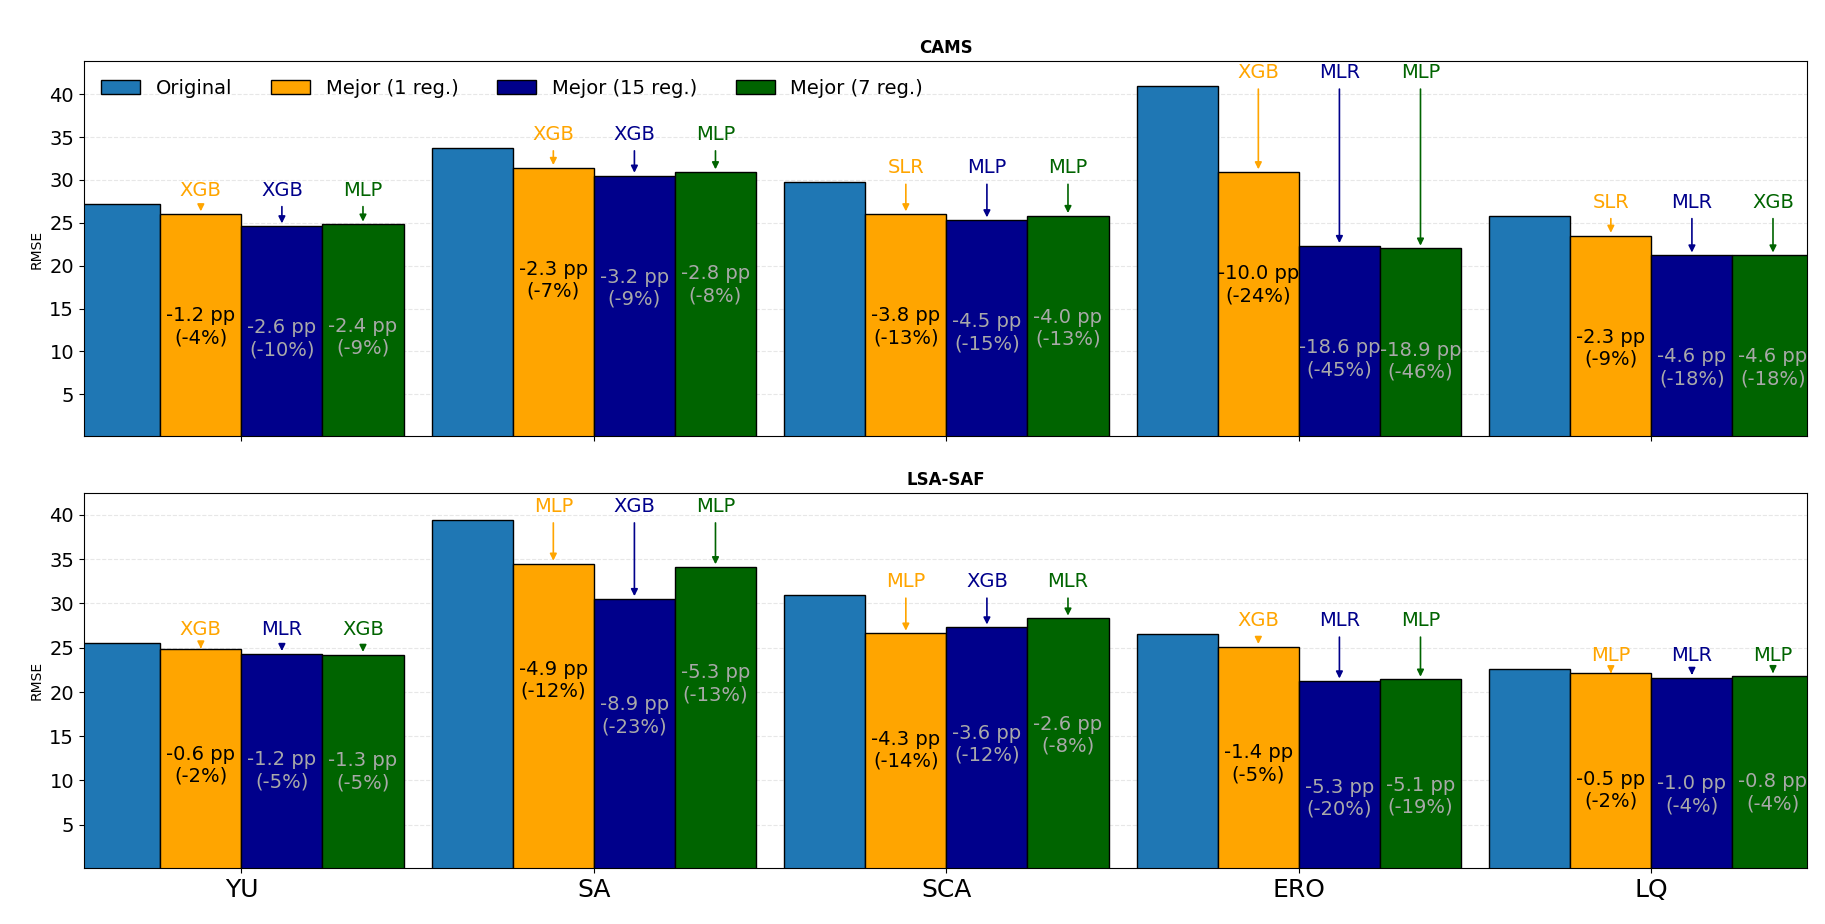
\includegraphics[width=\textwidth]{figuras/rmsd-multiple-mejor.png}
    \caption{Comparación del rendimiento entre el modelo original y los modelos ajustados con 15, 7 y 1 regresor en términos de RMSD. Las barras se muestran agrupadas por sitio y conjunto de datos, junto con flechas que indican la mejora o el deterioro con respecto al modelo original, así como deltas en puntos porcentuales (pp) y porcentaje relativo.}
    \label{fig:rrmsd-multiple}
\end{figure}


La Figura \ref{fig:rrmsd-multiple} muestra que incluso ante el mejor resultado que se puede obtener usando un conjunto amplio de variables regresoras se puede obtener un desempeño similar si toman algunas consideraciones sobre qué variables van a introducirse como fuentes descriptivas al modelo de regresiòn.\\



Por otro lado, pensamos que la selección de siete predictores representa un compromiso adecuado entre la simplicidad del modelo y su capacidad predictiva. Este subconjunto fue elegido considerando tanto los rankings de importancia de variables como los resultados de los análisis de selección de características, lo que permite capturar de manera consistente los factores que más influyen en la variabilidad del GHI, al tiempo que se minimiza la redundancia. La utilización de siete regresores facilita la retención de información clave proveniente de fuentes satelitales y meteorológicas, permitiendo una adaptación precisa por sitio sin incurrir en un elevado costo computacional. Como se observa en la Tabla~\ref{tab:metrics_7pred}, los modelos que emplean este conjunto de variables presentan valores de MAE entre 12 y 20\% y RMSE en el rango de 21–31\% del GHI promedio, lo que indica que un conjunto compacto puede ofrecer un desempeño comparable al de configuraciones más extensas, a la vez que mejora la interpretabilidad y la eficiencia del entrenamiento. No obstante, es importante reconocer que un análisis más profundo podría evaluar el impacto de reducir aún más el número de variables, especialmente en términos de precisión y generalización del modelo.\\












\section{Adaptación al sitio tomando consideraciones de una serie temporal}
En las Secciones \ref{sec:01} y \ref{sec:02} se han presentado las primeras evaluaciones del proceso de adaptación al sitio en la región del NOA, siguiendo enfoques previamente reportados en la literatura por distintos autores. Las implementaciones basadas en estos enfoques nos han proporcionado una base sólida para comprender la influencia del entorno local en la variable GHI, además hemos dimesionado cuales son los límites en la mejora que se puede obtener tras site adaptar una serie siguiendo estos enfoques.\\

En la presente sección se introducen los resultados obtenidos al aplicar un enfoque exploratorio desarrollado en esta tesis, basado en la desestacionalización de series temporales, con el objetivo de mejorar el proceso de adaptación al sitio (AS).

Una serie temporal se define como un conjunto de observaciones de una o más variables recolectadas y ordenadas cronológicamente. El orden temporal no es arbitrario, sino que es esencial para el análisis, la interpretación y la modelización de los datos, ya que permite identificar patrones, tendencias y comportamientos periódicos que pueden ser fundamentales para la toma de decisiones \cite{Olivas2022}.

El análisis de series temporales tiene aplicaciones en múltiples disciplinas. En Economía, permite estudiar la evolución de precios, la demanda de productos o la inflación. En Marketing, facilita la comprensión de la dinámica de ventas a lo largo del tiempo. En Medicina, las bioseñales, como el electrocardiograma (ECG), el electroencefalograma (EEG) o el electrooculograma (EOG), son ejemplos claros de series temporales utilizadas para diagnóstico y monitoreo de pacientes. Además, en la gestión hospitalaria, el análisis temporal puede aplicarse para evaluar la afluencia de pacientes a servicios de urgencias o la demanda de especialistas en diferentes períodos. Otro ámbito crucial es la meteorología, que constituye el foco principal de este trabajo. En este contexto, las series temporales permiten caracterizar, clasificar y predecir variables climáticas de interés, como la irradiancia global horizontal (GHI), entre otras.

Una característica clave de muchas series temporales es la estacionalidad, que se manifiesta cuando los datos muestran fluctuaciones regulares y predecibles con una frecuencia constante. Esta frecuencia puede ser diaria, semanal, mensual o anual, dependiendo del fenómeno que se estudie. Por ejemplo, en meteorología, la GHI presenta variaciones estacionales debidas a cambios en la posición del sol, la nubosidad o las condiciones atmosféricas. La presencia de estacionalidad puede influir significativamente en la interpretación y modelización de los datos, dado que introduce patrones repetitivos que podrían enmascarar otras tendencias o variaciones importantes.

El enfoque propuesto en esta tesis consiste en desestacionalizar las series temporales de GHI antes de aplicar el proceso de adaptación al sitio. La desestacionalización implica eliminar o ajustar estas fluctuaciones periódicas, de manera que se pueda analizar la serie en términos de su comportamiento subyacente, sin que las variaciones estacionales interfieran en la evaluación del proceso de AS. Este procedimiento permite comparar los datos en condiciones más homogéneas, mejorando la precisión y confiabilidad de los análisis.

En esta sección se evalúa el impacto de considerar la estacionalidad en la serie GHI sobre el proceso de AS, comparando el enfoque tradicional, que no realiza ajustes, con una metodología propuesta de desestacionalización.


En el proceso de \textbf{SA tradicional}, si consideramos como modelo de regresión al método \textbf{SLR}, que es el más simple de los distintos modelos disponibles, podemos expresar el proceso mediante la siguiente ecuación:

\begin{equation}
GHI_{\text{adaptada}} = a \cdot GHI_{\text{modelada}} + b,
\label{ec:approache1}
\end{equation}

donde \(GHI_{\text{adaptada}}\) representa la irradiancia global horizontal ajustada, \(GHI_{\text{modelada}}\) es la irradiancia modelada (por estimación satelital o re-análisis), y \(a\) y \(b\) son los coeficientes de regresión lineal, a este enfoque de ahora en más vamos a llamarlo Enfoque 1.\\

El Enfoque 2 se basa en la estrategia propuesta por \cite{ZAINALI2024}. En este enfoque, la variable regresora es el GHI modelado ($GHI_{\text{modelado}}$), y la variable objetivo se define como la diferencia entre el GHI medido y el modelado, es decir, 
$\Delta_{GHI} = GHI_{\text{medido}} - GHI_{\text{modelado}}$. Una vez obtenida la variable objetivo, el GHI adaptado se recupera sumando el factor de error $\Delta_{GHI}$ al GHI modelado.

\begin{align}
\Delta_{GHI} &= GHI_{\text{medido}} - GHI_{\text{modelado}} \\
GHI_{\text{adaptado}} &= GHI_{\text{modelado}} + (a \cdot \Delta_{GHI} + b)
\label{eq:approach2}
\end{align}


En este enfoque, la variable regresora se define como la diferencia entre el GHI modelado desestacionalizado, que se obtiene restando el GHI de cielo despejado del GHI modelado ($GHI_{\text{modelado}} - GHI_{\text{cielo despejado}}$). La variable objetivo corresponde a la diferencia entre el GHI medido desestacionalizado y el GHI de cielo despejado ($GHI_{\text{medido}} - GHI_{\text{cielo despejado}}$). Una vez estimada la variable objetivo, el valor corregido del GHI se recupera sumando nuevamente el GHI de cielo despejado.

\begin{align}
X &= GHI_{\text{modelado}} - GHI_{\text{cielo despejado}} \\
Y &= GHI_{\text{medido}} - GHI_{\text{cielo despejado}} \\
GHI_{\text{adaptado}} &= GHI_{\text{cielo despejado}} + (a \cdot X + b)
\label{eq:approach3}
\end{align}

En cada caso, los coeficientes $a$ y $b$ se obtienen mediante regresión lineal simple. El modelo de GHI de cielo despejado utilizado en este estudio es el modelo ARGP-V2 \cite{Ledesma2023a}.

\begin{figure*}[ht!]
\centering
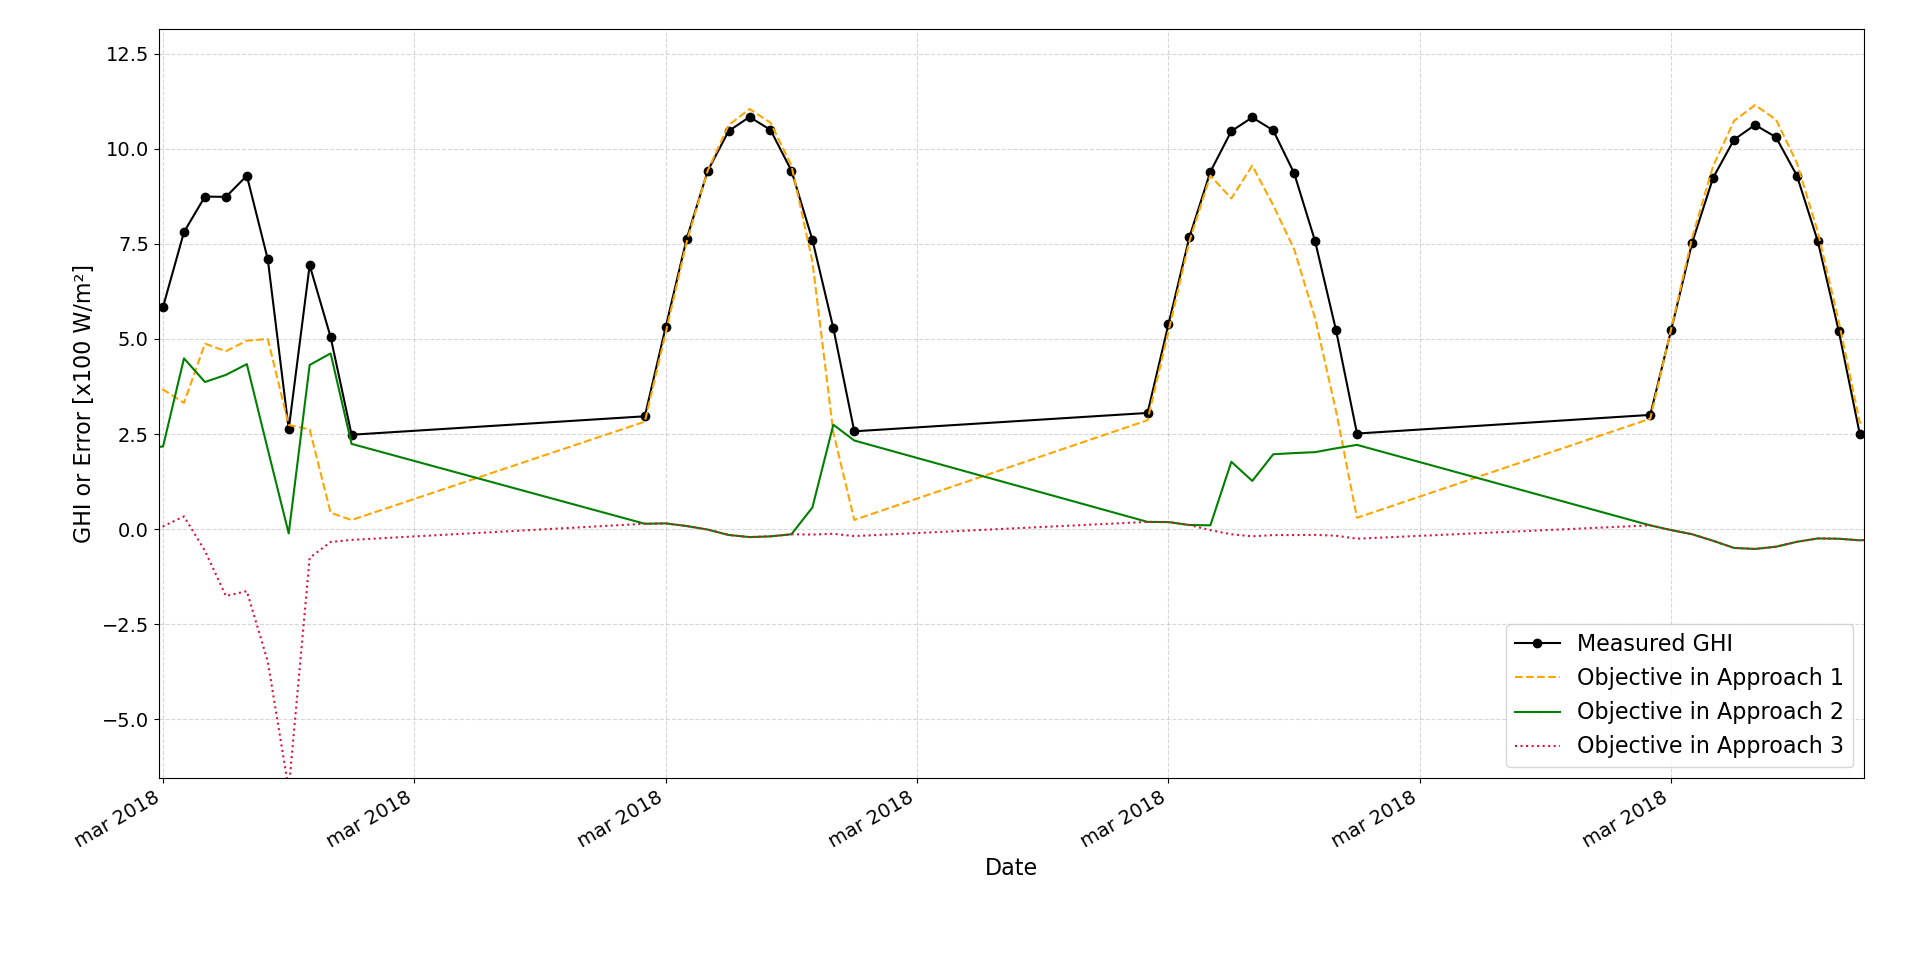
\includegraphics[width=\textwidth]{figuras/approaches.png}
\caption{Diferencias entre los tres enfoques de adaptación.}
\label{fig:approaches}
\end{figure*}



Los resultados obtenidos para cada uno de estos enfoques se presentan en la Tabla T. Cabe destacar que el Enfoque 1 fue el primero evaluado en esta tesis; para facilitar una comparación, se ha incluido también el reporte de las métricas correspondientes a este enfoque.


\begin{table*}
\caption{Métricas de desempeño (MBE, MAE, RMSE) para cada modelo en el conjunto de prubeas de los cinco sitios. Los valores están normalizados y expresados como porcentajes relativos a la media de GHI en cada sitio: 429.2~W/m$^2$ (Yu), 432.9~W/m$^2$ (Sa), 554.4~W/m$^2$ (Sca), 628.4~W/m$^2$ (Ero), y 648.7~W/m$^2$ (Lq). Los modelos etiquetados con ``(1 var.)'' indican adaptación al sitio realizada utilizando solo un regresor (CAMS o LSA-SAF).}
\label{tab:metricas_4_1}
\centering
\resizebox{\linewidth}{!}{
\def\arraystretch{1.5}
\begin{tabular}{cccccccccccccccc}
\hline
      & \multicolumn{3}{c}{Yu} & \multicolumn{3}{c}{Sa} & \multicolumn{3}{c}{Sca} & \multicolumn{3}{c}{Ero} & \multicolumn{3}{c}{Lq} \\
Modelo & MBE & MAE & RMSE & MBE & MAE & RMSE  & MBE & MAE & RMSE & MBE & MAE & RMSE & MBE & MAE & RMSE  \\
\hline
\multicolumn{16}{|c|}{\textit{Estimaciones satelitales en bruto}} \\
\hline
CAMS    & -0.2 & 17.4 & 27.2 &  3.9 & 23.4 & 33.7 &  2.6 & 21.8 & 29.8 & -23.6 & 27.6 & 40.9 & -6.9 & 16.5 & 25.8 \\
LSA-SAF &  7.6 & 16.5 & 25.5 & 17.9 & 27.4 & 39.4 & 13.1 & 22.2 & 30.9 &  -7.7 & 16.2 & 26.5 &  4.0 & 12.6 & 22.6 \\
\hline

\multicolumn{16}{|c|}{\textit{Adaptación al sitio con un solo regresor (1 var.)}} \\
\hline
SLR-CAMS    & -0.9 & 17.1 & 26.4 &  3.8 & 21.3 & 31.5 & -1.5 & 18.4 & 26.0 &  2.5 & 24.8 & 31.5 &  2.1 & 15.9 & 23.5 \\
XGB-CAMS (1 var.) & -1.3 & 17.1 & 26.0 &  3.8 & 21.4 & 31.4 & -1.8 & 18.9 & 26.2 &  2.5 & 23.9 & 30.9 &  2.2 & 15.9 & 23.5 \\
MLP-CAMS (1 var.) & -4.4 & 17.7 & 26.2 &  4.8 & 21.4 & 31.6 &  7.7 & 17.8 & 27.7 &  0.5 & 24.1 & 31.2 &  9.1 & 19.4 & 25.6 \\
SLR-LSASAF  & -5.5 & 18.4 & 25.0 &  4.4 & 23.9 & 34.6 &  1.0 & 18.0 & 26.7 &  2.7 & 17.1 & 25.4 &  2.2 & 12.9 & 22.3 \\
XGB-LSASAF (1 var.) & -6.0 & 18.2 & 24.9 &  4.3 & 23.9 & 34.6 &  0.5 & 18.6 & 27.0 &  2.4 & 17.2 & 25.1 &  2.3 & 13.1 & 22.3 \\
MLP-LSASAF (1 var.) & -7.1 & 18.6 & 25.0 &  4.5 & 23.6 & 34.5 &  5.9 & 18.4 & 26.6 &  2.5 & 17.0 & 25.3 & -0.4 & 13.6 & 22.1 \\
\hline
\multicolumn{16}{|c|}{\textit{Adaptación al sitio con 15 regresores}} \\
\hline
MLR-CAMS    & -3.9 & 17.0 & 25.3 &  3.8 & 20.9 & 30.9 &  0.7 & 18.8 & 26.9 &  0.6 & 14.4 & 22.3 &  3.8 & 12.8 & 21.2 \\
XGB-CAMS    & -3.4 & 16.4 & 24.6 &  3.3 & 20.1 & 30.5 & -1.3 & 19.8 & 27.3 &  0.5 & 13.8 & 22.4 &  2.1 & 12.9 & 21.8 \\
MLP-CAMS    &  0.1 & 19.4 & 29.4 &  0.9 & 23.7 & 36.7 &  3.1 & 20.3 & 31.2 & -0.4 & 16.1 & 27.3 &  2.7 & 14.9 & 24.7 \\
MLR-LSASAF  & -5.5 & 16.9 & 24.3 &  4.0 & 23.5 & 33.8 & -0.2 & 21.0 & 28.6 &  0.9 & 13.5 & 21.2 &  1.6 & 13.0 & 21.6 \\
XGB-LSASAF  & -5.3 & 16.5 & 24.6 &  3.6 & 23.1 & 30.5 & -1.0 & 21.8 & 27.3 &  0.7 & 13.1 & 22.4 &  1.8 & 13.4 & 21.8 \\
MLP-LSASAF  & -4.9 & 21.9 & 32.2 &  3.5 & 27.1 & 40.7 & -3.7 & 21.0 & 29.7 &  0.8 & 15.1 & 25.8 &  4.5 & 15.3 & 25.3 \\
\hline
\end{tabular}}
\end{table*}





\section{Adaptación al sitio usando celdas satelitáles adyacentes al sitio de interés}
Las evaluaciones realizadas en este trabajo y en estudios previos sobre SA se han basado exclusivamente en datos medidos en una estación meteorológica. Estos datos se combinan con una o más variables modeladas —provenientes de una celda satelital o de un modelo de reanálisis— que representan geográficamente la ubicación de dicha estación. En otras palabras, la información utilizada para entrenar y validar los modelos de corrección se limita a la celda específica del punto de medición, sin considerar el contexto espacial más amplio que podría aportar información adicional relevante.\\

Los enfoques previos de SA aplicados a mediciones terrestres de una estación enfrentan una limitación intrínseca: la información derivada de los productos satelitales es finita, lo que restringe la capacidad de aprendizaje de cualquier técnica de aprendizaje automático implementada, incluso sin sobreajuste. Para superar esta restricción, proponemos un enfoque que amplía el alcance espacial de los datos de entrada incorporando valores de GHI modelados de celdas satelitales adyacentes. La hipótesis central es que la variabilidad de la irradiancia solar en un punto no es aislada, sino que forma parte de una estructura espacialmente coherente gobernada por la dinámica atmosférica regional. Al incluir las estimaciones de irradiancia de celdas vecinas como predictores adicionales, el modelo dispone de información espacial más rica, mejorando su capacidad para identificar patrones complejos y generalizar de manera más efectiva.\\

Este enfoque aprovecha correlaciones bien documentadas en los campos de irradiancia solar, impulsadas por el movimiento de nubes, el transporte de aerosoles y los sistemas meteorológicos a escala sinóptica \citep{IHSAN2024}. A diferencia de los métodos tradicionales de AS, que se limitan a variables locales dentro de una sola celda, el marco propuesto utiliza de manera innovadora la irradiancia satelital de las celdas circundantes como características de entrada para los modelos de aprendizaje automático. Hasta ahora, ningún trabajo había explorado explícitamente esta integración del contexto espacial.



Este enfoque puede explicarse a partir de la Figura \ref{fig:gridSA}



\begin{figure}
    \centering
    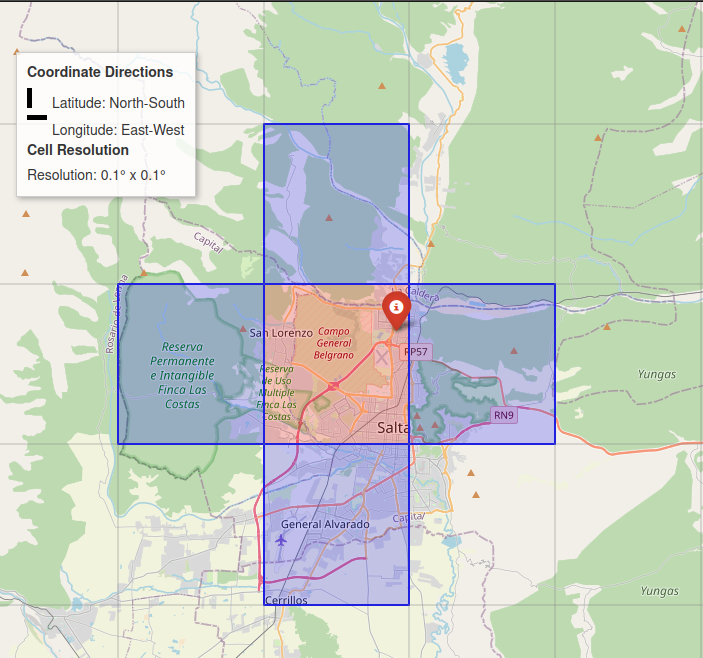
\includegraphics[width=0.9\textwidth]{figuras/gridSA.png}
    \caption{Grilla }
    \label{fig:gridSA}
\end{figure}


 %Obligatorio
\lhead{Conclusiones}
\rhead{\newtitle}
\cfoot{\thepage}
\renewcommand{\headrulewidth}{1pt}
\renewcommand{\footrulewidth}{1pt}
\chapter{Conclusiones}
\noindent Se escriben las conclusiones del trasasdabajo. %Obligatorio
 

\rhead{\newtitle}
\cfoot{\thepage}
\renewcommand{\headrulewidth}{1pt}
\renewcommand{\footrulewidth}{1pt}



\bibliographystyle{plainnat}  % Cambia el estilo si lo necesitas (plain, alpha, apalike, etc.)
\bibliography{bibliografia}  % Usa el nombre del archivo .bib (sin la extensión)
 %Obligatorio
\addcontentsline{toc}{chapter}{\textbf{Anexo 1}} 
\lhead{Anexo 1}
\rhead{\newtitle}
\cfoot{\thepage}
\renewcommand{\headrulewidth}{1pt}
\renewcommand{\footrulewidth}{1pt}
\chapter*{Anexo 1}
\noindent Se escribe el anexo correspondiente. %Opcional: Comentar si se desea

\end{document}